\documentclass[11pt,a4paper]{article}

\usepackage[margin=2.4cm]{geometry}
\usepackage[T1]{fontenc}
\usepackage{lmodern}
\usepackage{amsmath,amssymb,bm,mathtools}
\usepackage{graphicx}
\usepackage{booktabs}
\usepackage{tabularx}
\usepackage{longtable}
\usepackage{array}
\usepackage{caption}
\usepackage{float}
\usepackage{xcolor}
\usepackage{enumitem}
\usepackage{listings}
\usepackage[most]{tcolorbox}
\usepackage{tikz}
\usetikzlibrary{arrows.meta,positioning,calc,shapes.geometric}
\usepackage[numbers,sort&compress]{natbib}
\usepackage[colorlinks=true,linkcolor=blue!50!black,citecolor=blue!50!black,urlcolor=blue!50!black]{hyperref}

\captionsetup{font=small,labelfont=bf}
\newcolumntype{L}{>{\raggedright\arraybackslash}X}
\newcommand{\vect}[1]{\boldsymbol{#1}}
\newcommand{\Ts}{T_{\mathrm{s}}}
\setlist{itemsep=2pt,topsep=4pt}
\setcounter{tocdepth}{2}

% "In plain words" boxes and "Jargon" boxes
\newtcolorbox{plain}[1][In plain words]{colback=blue!3,colframe=blue!45!black,fonttitle=\bfseries\small,title=#1,boxrule=0.6pt,arc=2pt,left=6pt,right=6pt,top=4pt,bottom=4pt}
\newtcolorbox{jargon}[1]{colback=orange!4,colframe=orange!60!black,fonttitle=\bfseries\small,title={Term: #1},boxrule=0.6pt,arc=2pt,left=6pt,right=6pt,top=4pt,bottom=4pt}
\newtcolorbox{codebox}[1]{colback=gray!4,colframe=gray!55!black,fonttitle=\bfseries\small,title={In the code: #1},boxrule=0.6pt,arc=2pt,left=6pt,right=6pt,top=4pt,bottom=4pt}

\lstset{language=Python,basicstyle=\ttfamily\footnotesize,keywordstyle=\color{blue!60!black}\bfseries,
  commentstyle=\color{green!35!black}\itshape,stringstyle=\color{orange!60!black},columns=fullflexible,
  keepspaces=true,showstringspaces=false,frame=none,breaklines=true,xleftmargin=4pt,aboveskip=4pt,belowskip=2pt}

\title{Fault-Tolerant Control of a Quadrotor\\ After Complete Rotor Loss\\[0.3em]
\Large Residual Koopman MPC and\\ Fault-Detection-Delay Limits\\[0.8em]
\large EE650 Basics of Modern Control Systems: Detailed Project Report}
\author{\begin{tabular}{ll}
Pranshu Kumar (220799) & Mudita Jain (220675)\\
Prashant Gupta (220803) & Aarush Singh Kushwaha (230019)
\end{tabular}}
\date{October 2026}

\begin{document}
\maketitle

\begin{abstract}
When one rotor of a quadrotor (a drone with four propellers) stops completely, the drone can no longer hover level. The only steady way it can still fly is to spin continuously about a slightly tilted axis. Mueller and D'Andrea called this state the \emph{relaxed hover} and showed that it can be controlled. This project studies, in simulation, how to bring a drone into this spinning state reliably after a rotor fails.

We ask two connected questions. \textbf{First}, the physics model of the spinning drone is good but not perfect: can we keep it and learn only its error from data, with the tools of Koopman methods, and does this predict and control better than the physics model alone or a Koopman model of the full dynamics? \textbf{Second}, a fault detector needs time to notice the failure: how long may this take before a safe recovery is no longer possible, and can such a limit be guaranteed mathematically?

Our simulator of the Mueller--D'Andrea drone reproduces their two-rotor and three-rotor-loss equilibria to every published digit, five hover solutions of their more detailed model within 4\%, and the spin-up time of their flight within about 4\%. For prediction horizons from 100\,ms to 1\,s, the model that learns only the error (the \emph{residual} model) is the most accurate predictor on the plant it was trained on, and with 10 training episodes it beats a full Koopman model trained on 40. Inside model predictive control (MPC) it reduces a steady altitude error caused by model mismatch by about one third. The learned models do not yet work on a plant with different parameters. In our simulation, the published recovery strategy recovers safely with probability above 0.9 only if the failure is detected within about 12\,ms, and below 0.5 beyond about 19\,ms, while published detectors need about 20 to 130\,ms. A first certificate, valid for the linearized model with thrust limits and based on linear matrix inequalities, covers 22\% of the way from the spinning equilibrium to the state right after a failure.

Technical terms are explained where they first appear and are collected in a glossary (Appendix~\ref{app:glossary}). Each method is described in three layers: the idea in plain words, the mathematics, and how it is implemented in our code.
\end{abstract}


\tableofcontents
\newpage

%=====================================================================
\section{Introduction}\label{sec:intro}
%=====================================================================

\subsection{How a quadrotor flies}
A quadrotor has four propellers, each driven by its own electric motor. Each propeller pushes air down and so produces an upward force called \emph{thrust}. A quadrotor has no wings and no rudder: everything it does, it does by changing the four thrusts.
\begin{itemize}
  \item \textbf{Going up and down.} If all four thrusts together are larger than the weight, the drone climbs; if smaller, it descends.
  \item \textbf{Tilting (roll and pitch).} If the propeller on one side pushes harder than the one on the opposite side, the drone tilts. A tilted drone has its thrust pointing partly sideways, so it moves sideways. This is how a quadrotor travels horizontally.
  \item \textbf{Turning (yaw).} A spinning propeller also pushes back on the drone with a small twisting effect (a \emph{reaction torque}), in the direction opposite to its spin. Two of the propellers spin clockwise and two anticlockwise, so in normal flight the twisting effects cancel. To turn, the drone speeds up the pair that spins one way and slows down the other pair.
\end{itemize}
Four thrusts control exactly four things: total upward force, roll, pitch and yaw. There is no spare actuator. This is why losing even one rotor is serious.

\subsection{What happens when a rotor fails}
If one rotor stops completely, only three thrusts remain, but the drone still needs to (i) carry its weight, (ii) keep from rolling over and (iii) cancel the yaw twist. With three propellers this is impossible: the reaction torques of the remaining propellers no longer cancel, so the drone starts to spin about its vertical axis, faster and faster, until air drag on the spinning body balances the twist.

Mueller and D'Andrea showed that this is not the end~\cite{mueller2014stability,mueller2016relaxed}. If we \emph{give up} control of the yaw angle (the compass heading) and accept that the drone spins, the remaining three rotors can still hold the drone in the air and steer it. For their drone the paper predicts a constant spin of about 20\,rad/s (about 3 turns per second) around an axis tilted about 17$^\circ$ from the body's vertical axis, while the centre of mass moves on a tiny circle of about 8\,mm radius (our simulator gives 19.6\,rad/s, 16$^\circ$ and 7\,mm; Section~\ref{sec:validation} explains the small difference). They called this state the \emph{relaxed hover}, and they flew it on a real drone.

\begin{plain}
Think of a spinning top. It cannot stand still upright, but it can stand steadily while spinning. After losing a rotor the drone becomes something like a flying spinning top: it is stable only while it spins, and it moves around by tilting its spin axis.
\end{plain}

\subsection{The two problems this project studies}
Getting a real drone into this spinning state raises two connected problems.

\paragraph{Problem 1: the model is not perfect.} A controller is designed using a mathematical model of the drone. The physics model of Mueller and D'Andrea captures the main spinning motion well, but it misses some real effects. For example, in their two-propeller flight the drone stayed about 2.4\,m below its set-point, which the authors attribute to less thrust while spinning fast, and in the one-propeller flights the drone spun about 20 to 27\% slower than predicted~\cite{mueller2014stability,mueller2016relaxed}; the inertia and motor speed are never known exactly. A controller built on an imperfect model makes systematic errors, for example it settles at the wrong height. A natural fix is to keep the physics model and \emph{learn its error} from data. We learn the error with the tools of Koopman methods (EDMD, Section~\ref{sec:background}): a fixed dictionary of nonlinear features of the state and input, and least-squares regression. In the controller the learned correction is evaluated outside the optimization, as Todde et al.\ do~\cite{todde2026residual}, so the optimization problem stays easy (convex) to solve. Such ``residual Koopman'' models already exist for healthy drones and other robots~\cite{todde2026residual,bruder2025residual,narayanan2026rkmpc}, but we did not find them applied to the spinning state after a complete rotor loss.

\paragraph{Problem 2: detection takes time.} The flight computer does not know immediately that a rotor has failed. A fault-detection algorithm has to notice it first, and published detectors need about 20 to 130\,ms~\cite{strack2021fast,yang2026mml1,zhou2025rotorfailureaware}. During this time the normal (healthy-flight) controller keeps flying a drone that has lost a rotor, and the drone tilts and drops. When the failure is finally detected, the failure-mode controller must catch the drone from wherever it has drifted. Several recovery methods that come with a mathematical guarantee start their analysis at the moment the failure is known and do not model the undetected interval~\cite{simha2017geometric,allawati2026quasi}, and many studies assume the failure is known in advance~\cite{zhou2025rotorfailureaware}. For linear systems whose remaining actuators can still compensate a fault, LMI methods exist that maximize the tolerated detection delay under actuator saturation~\cite{rotondo2015virtual,rotondo2016virtual}. For complete rotor loss of a quadrotor, where the steady state after the failure is a spin, we did not find a certified \emph{maximum} tolerable detection delay that accounts for the limited thrust of real motors.

\subsection{Research questions}
\begin{description}[leftmargin=1.2em]
  \item[RQ1 (as proposed).] Can a Koopman-style (EDMD) model of only the mismatch, built on top of the known spinning-equilibrium model of Mueller and D'Andrea, predict and control the failed drone better than the physics model alone, or than a Koopman model of the full dynamics? ``Better'' means a smaller multi-step prediction error on new data, and a smaller steady error in closed loop.
  \item[RQ2 (added after the proposal).] What is the largest fault-detection delay $\tau^\star$ for which recovery into the spinning state can be guaranteed mathematically (as a first step, for the linearized model with thrust limits), given the healthy controller, the failure-mode controller, thrust limits, motor lag and sampling? How do the controllers of RQ1 change $\tau^\star$?
\end{description}
The two questions are linked: every controller that catches the drone after detection (LQR, analytical MPC, residual Koopman MPC) can be compared by the detection delay it tolerates.

\paragraph{Hypotheses.} Before the experiments we wrote down what we expected:
\begin{description}[leftmargin=1.2em,itemsep=1pt]
  \item[H1.] A Koopman model of the full failed-drone dynamics has eigenvalues outside the unit circle and loses to a ``nothing changes'' predictor at long horizons.
  \item[H2.] The residual model has a smaller multi-step prediction error than both the physics model and the full Koopman model.
  \item[H3.] An MPC that uses the residual removes the steady error that model mismatch causes in an MPC built on the physics model.
  \item[H4.] The residual model reaches a given prediction error with less training data than the full Koopman model.
  \item[H5.] A certificate built from the linearization at the spinning equilibrium does not cover the state right after a failure; one valid over the whole spin-up does.
  \item[H6.] The certified $\tau^\star$ is finite and of the same order as real detector delays.
  \item[H7.] The certified $\tau^\star$ is within 2 to 3 times the delay found by simulation.
\end{description}
H1 to H4 belong to RQ1 and H5 to H7 to RQ2. Section~\ref{sec:discussion} gives the status of each.

\subsection{What we did}
Everything is done in simulation; no hardware is used. In order:
\begin{enumerate}
  \item We wrote a simulator of the drone used by Mueller and D'Andrea (Sections~\ref{sec:model} and~\ref{sec:code}).
  \item \textbf{V0, E1:} we checked it against three published papers, against flight data and against hand-derived physics results (Section~\ref{sec:validation}).
  \item \textbf{E2, E3:} we analysed the linearized models (controllability, observability) and designed LQR controllers (Section~\ref{sec:linear}).
  \item \textbf{E6:} we built three predictors of the failed drone (physics only, full Koopman, residual Koopman) and compared them (Section~\ref{sec:koopman}).
  \item \textbf{E7:} we built MPC controllers on the physics model with and without the learned residual (Section~\ref{sec:mpc}).
  \item \textbf{E4:} we measured how the probability of a safe recovery falls as detection takes longer (Section~\ref{sec:delay}).
  \item \textbf{E5:} we computed a first mathematical certificate (an LMI-based invariant ellipsoid) and compared it with simulation (Section~\ref{sec:certificate}).
\end{enumerate}
The labels V0 and E1 to E7 are the experiment names used in figure titles and in the code (Appendix~\ref{app:repro}).

\paragraph{What is reproduction and what is new.} The model, the equilibrium, its controllability, the LQR weights and the spin-up strategy are from Mueller and D'Andrea; we reimplemented and checked them, and found one inconsistency in a published case. New in this work, as far as our search found: the comparison of physics-only, full Koopman and residual models in the spinning regime after complete rotor loss and its use in MPC (RQ1); the idle-thrust argument and the measured probability of safe recovery against detection delay; and the first saturation-aware certificate for this controller, as a step towards a certified delay budget (RQ2).
Section~\ref{sec:discussion} discusses the results, the limitations and the remaining work. Appendix~\ref{app:glossary} is a glossary of all technical terms, Appendix~\ref{app:symbols} lists the symbols, and Appendix~\ref{app:repro} explains how to reproduce every number.

\subsection{Main results in one table}
\begin{table}[H]
\centering\small
\caption{Main results so far. Details and caveats are in the sections given.}\label{tab:main}
\begin{tabularx}{\linewidth}{l L l}
\toprule
Topic & Result & Section \\
\midrule
Simulator validation & Two-rotor and three-rotor-loss equilibria of~\cite{mueller2014stability} reproduced to every published digit; five cases of~\cite{mueller2016relaxed} within 4\%; flight spin-up time within 4\% & \ref{sec:validation} \\
Linear analysis & Failed drone is controllable from three rotors; gyroscopes alone cannot see tilt or height & \ref{sec:linear} \\
LQR baseline & Recovers on the nonlinear model; tolerates only 18\,ms of input delay (healthy LQR: 40\,ms) & \ref{sec:linear} \\
Prediction (RQ1) & Residual model best from 100\,ms to 1\,s (1\,s error 0.64 vs 0.91 full Koopman vs 7.09 physics only); needs less data & \ref{sec:koopman} \\
Generalization (RQ1) & Learned models fail on a plant with different parameters & \ref{sec:koopman} \\
MPC (RQ1) & Residual Koopman MPC cuts the steady altitude error by 32\% on the training plant; on one held-out variant (plant B without its thrust loss) the error is 47\% larger & \ref{sec:mpc} \\
Detection delay (RQ2) & Safe-recovery probability below 0.9 from 12\,ms and below 0.5 from 19\,ms of delay & \ref{sec:delay} \\
Certificate (RQ2) & For the linearized model with thrust limits: certified 22\% of the way to the failure state; simulation recovers up to 70\% & \ref{sec:certificate} \\
\bottomrule
\end{tabularx}
\end{table}

%=====================================================================
\section{Background: the ideas we use}\label{sec:background}
%=====================================================================
This section explains, in simple terms, the ideas from control theory, numerical computing and machine learning that the rest of the report uses. A reader who knows them can skip to Section~\ref{sec:literature}. Each idea is revisited with its exact equations where it is used.

\subsection{Systems, states, inputs and outputs}
A \emph{system} is anything whose behaviour changes over time and can be influenced: here, the drone. Its \emph{state} $\vect x$ is the smallest list of numbers that, together with future inputs, determines its future. For a drone the state contains position, velocity, orientation (attitude), rotation rates and, because motors cannot change speed instantly, the current thrust of each motor. The \emph{inputs} $\vect u$ are what we command: the four thrusts. The \emph{outputs} $\vect y$ are what sensors measure.

A \emph{state-space model} writes the system as a differential equation
\begin{equation}
  \dot{\vect x}(t) = f(\vect x(t), \vect u(t)), \qquad \vect y(t) = h(\vect x(t)),
\end{equation}
where the dot means the rate of change in time. The function $f$ comes from physics (Newton's laws). If $f$ has the special form $A\vect x + B\vect u$ with constant matrices $A$ and $B$, the model is \emph{linear time-invariant} (LTI). Linear models are much easier to analyse and to control, so a large part of control theory is about them.

\subsection{Equilibria and linearization}
An \emph{equilibrium} (also called a \emph{trim point}) is a pair $(\bar{\vect x},\bar{\vect u})$ at which nothing changes: $f(\bar{\vect x},\bar{\vect u})=0$. For a healthy drone, hover with each motor carrying a quarter of the weight is an equilibrium. For a drone with a failed rotor, the relaxed hover is an equilibrium, but only in coordinates that rotate with the drone (Section~\ref{sec:model}).

Close to an equilibrium, a smooth nonlinear model behaves almost like a linear one. Writing small deviations $\delta\vect x = \vect x - \bar{\vect x}$ and $\delta\vect u = \vect u - \bar{\vect u}$, a first-order Taylor expansion gives
\begin{equation}
  \delta\dot{\vect x} \approx A\,\delta\vect x + B\,\delta\vect u, \qquad
  A = \frac{\partial f}{\partial\vect x}\Big|_{\bar{\vect x},\bar{\vect u}}, \quad
  B = \frac{\partial f}{\partial\vect u}\Big|_{\bar{\vect x},\bar{\vect u}} .
\end{equation}
The matrices of partial derivatives $A$ and $B$ are called \emph{Jacobians}, and the process is called \emph{linearization}. We compute the Jacobians numerically by \emph{central differences}: change one entry of $\vect x$ by a tiny amount $\epsilon$ up and down and divide the change in $f$ by $2\epsilon$.

\subsection{Eigenvalues and stability}
The behaviour of $\dot{\vect x}=A\vect x$ is described by the \emph{eigenvalues} $\lambda$ of $A$ (numbers with $A\vect v = \lambda\vect v$ for some vector $\vect v$). Each eigenvalue is a \emph{mode}: a pattern of motion that grows or decays like $e^{\lambda t}$.
\begin{itemize}
  \item Real part negative: the mode decays (stable). The more negative, the faster.
  \item Real part positive: the mode grows (unstable).
  \item Real part zero: a simple (non-repeated) eigenvalue gives a mode that neither grows nor decays (marginally stable), for example an undamped oscillation or a single integrator. A repeated zero eigenvalue that forms a chain, such as the double integrator from force to position, grows linearly in time and is therefore unstable.
  \item Imaginary part $\pm j\omega$: the mode oscillates with angular frequency $\omega$\,rad/s.
\end{itemize}
The \emph{damping ratio} $\zeta = -\operatorname{Re}\lambda/|\lambda|$ of an oscillating mode says how quickly the oscillation dies out: $\zeta=1$ means no overshoot, $\zeta$ near 0 means a long ringing.

\paragraph{Discrete time.} Computers act at fixed time steps of length $\Ts$ (the \emph{sample period}). A discrete-time model is $\vect x_{k+1} = A_d\vect x_k + B_d\vect u_k$, where $k$ counts steps. If the input is held constant between samples (a \emph{zero-order hold}, ZOH), the exact discrete matrices are $A_d=e^{A\Ts}$ and $B_d = \int_0^{\Ts}e^{As}\,ds\,B$. In discrete time a mode is stable if its eigenvalue lies inside the unit circle, $|\lambda|<1$. The largest $|\lambda|$ is the \emph{spectral radius}; a value above 1 means some prediction errors grow at every step.

\subsection{Numerical simulation}
The nonlinear equations cannot be solved by hand, so we integrate them step by step. We use the classical fourth-order \emph{Runge--Kutta} method (RK4): in each step of length $\Delta t$ it evaluates $f$ four times (at the start, twice at the middle, at the end) and takes a weighted average. Its error per unit time shrinks like $\Delta t^4$, so halving the step makes the error about 16 times smaller. We use $\Delta t$ = 0.5 to 1\,ms, much shorter than the fastest motion of the drone.

\subsection{Feedback control and LQR}
A \emph{feedback controller} measures the state and computes the input from it, for example $\vect u = -K\vect x$ with a \emph{gain matrix} $K$. The closed loop is then $\dot{\vect x} = (A-BK)\vect x$, and the job of control design is to choose $K$ so that all eigenvalues of $A-BK$ have negative real parts with good damping.

The \emph{linear-quadratic regulator} (LQR) chooses $K$ by minimizing a cost
\begin{equation}
  J = \int_0^\infty \big(\vect x^\top Q\vect x + \vect u^\top R\vect u\big)\,dt,
\end{equation}
where the weight matrix $Q$ penalizes state errors and $R$ penalizes control effort. Large $Q$ entries make the controller aggressive on those states; large $R$ makes it gentle on the motors. The optimal gain is $K = R^{-1}B^\top P$, where $P$ solves the \emph{algebraic Riccati equation} $A^\top P + PA - PBR^{-1}B^\top P + Q = 0$. A common way to choose the weights is \emph{Bryson's rule}: $Q_{ii} = 1/(\text{largest acceptable error in state } i)^2$ and similarly for $R$.

\subsection{Controllability and observability}
A system is \emph{controllable} if the inputs can move the state from anywhere to anywhere. For an LTI system this holds exactly when the \emph{controllability matrix} $[B, AB, A^2B,\dots,A^{n-1}B]$ has full rank $n$ (the number of states). (The rank is computed from the \emph{singular values} of the matrix, which measure how much it stretches vectors in each direction; a singular value near zero means a direction it almost loses.) The \emph{PBH test} (Popov--Belevitch--Hautus) checks the same property mode by mode: mode $\lambda$ is controllable if the matrix $[\lambda I - A,\; B]$ has full rank.

A system is \emph{observable} if the state can be worked out from the sensor outputs over time. The test is the same with $(A^\top, C^\top)$ in place of $(A, B)$, where $\vect y = C\vect x$. A rank test only says yes or no. To say \emph{how well} a direction can be seen or reached, we use \emph{Gramians}: the observability Gramian $W_o(T)=\int_0^T e^{A^\top s}C^\top C e^{As}ds$ measures how much output ``energy'' each initial state produces in time $T$. A tiny smallest eigenvalue means a direction that is almost invisible to the sensors.

\subsection{Model predictive control (MPC)}
MPC repeatedly solves a small optimization problem. At every sample it uses a model to predict the next $N$ steps (the \emph{horizon}), chooses the input sequence that minimizes a cost (like the LQR cost) while respecting limits (for example motor thrust limits), applies only the first input, and repeats at the next sample with a new measurement. Re-solving at every step from a new measurement adds feedback: a prediction error made at one step is corrected at the next.

When the model is linear, the cost quadratic and the limits linear, the optimization is a \emph{quadratic program} (QP). With a positive definite weight on the inputs (as in our MPC) the QP is \emph{strictly convex}: it has a single best solution, and solvers find it reliably and fast. Keeping the problem convex is the main reason we want linear prediction models.

\subsection{Saturation and delay}
Real motors have limits. \emph{Saturation} means that a command outside the range $[f_{\min}, f_{\max}]$ is clipped. A controller that asks for more than the motors can give behaves differently from its linear design, and can even become unstable. \emph{Delay} means that the controller acts on old information. Every feedback loop tolerates only a certain pure delay before it becomes unstable; this amount is its \emph{delay margin}.

\subsection{Koopman operators and EDMD}
The \emph{Koopman operator} is a way to describe a nonlinear system with linear equations. Instead of following the state $\vect x$ itself, one follows many functions of it, $\psi_1(\vect x), \psi_2(\vect x),\dots$ (called \emph{observables}, collected into a \emph{dictionary}). For a system without inputs and a well-chosen, possibly infinite, set of observables, their evolution is exactly linear. In practice one uses a finite dictionary (for example all products of pairs of states) and finds the best linear map from data, so the result is an approximation; with inputs, the lifted model below is an approximation even for a rich dictionary~\cite{korda2018linear}. This is \emph{extended dynamic mode decomposition} (EDMD)~\cite{williams2015edmd}; its extension to inputs~\cite{korda2018linear} we call EDMDc. The resulting model, $\vect z_{k+1} = A\vect z_k + B\vect u_k$ with $\vect z = \psi(\vect x)$, is linear in a bigger \emph{lifted} state $\vect z$, so it can be used directly in a convex MPC.

\begin{plain}
Imagine predicting the motion of a ball on a curved track. Its position alone changes in a complicated, nonlinear way. But if you also keep track of its speed, the square of its speed, its height and so on, the rules that update all these numbers together can be close to a simple linear recipe. Koopman methods look for such a set of numbers and the recipe that updates them.
\end{plain}

\subsection{Regression, ridge regression and residual learning}
\emph{Linear regression} finds a matrix $W$ so that $\vect y\approx W^\top\vect\phi$ for many examples $(\vect\phi,\vect y)$, by minimizing the sum of squared errors. \emph{Ridge regression} adds a small penalty $\lambda\|W\|^2$; this keeps $W$ from becoming huge when some features are nearly duplicates, and reduces \emph{overfitting} (fitting the noise of the training data instead of the true pattern). The solution has the closed form $W = (\Phi^\top\Phi + \lambda I)^{-1}\Phi^\top Y$.

\emph{Residual learning} keeps a trusted model and learns only what it gets wrong. If the physics model predicts $\vect x^{\text{nom}}_{k+1}$ and the truth is $\vect x_{k+1}$, the learned part predicts the \emph{residual} $\vect e_{k+1} = \vect x_{k+1} - \vect x^{\text{nom}}_{k+1}$. The hope is that the residual is small and simple, so it can be learned from little data.

\subsection{Lyapunov functions and linear matrix inequalities}
A \emph{Lyapunov function} $V(\vect x)$ is like an energy: it is zero at the equilibrium, positive elsewhere, and always decreases along the motion of the system. If such a function exists, the system returns to the equilibrium. A common choice is $V = \vect x^\top P\vect x$ with a \emph{positive definite} matrix $P$ (written $P\succ0$), which means $\vect x^\top P\vect x>0$ for every $\vect x\ne0$; $P\succeq0$ (positive semidefinite) allows equality, and $P\preceq0$ means $-P\succeq0$. The set where $V\le1$ is an \emph{ellipsoid}; if $V$ decreases everywhere on it, no trajectory can leave it, so it is an \emph{invariant set}, and every state inside it is guaranteed to recover.

A \emph{linear matrix inequality} (LMI) is a condition of the form ``this symmetric matrix, which depends linearly on unknown matrices, is negative (or positive) semidefinite''. The conditions for a Lyapunov function can often be written as LMIs. LMIs are convex, so a computer can find the largest certified ellipsoid reliably~\cite{boyd1994lmi}. Section~\ref{sec:certificate} explains this in detail.

\subsection{Statistics used}
\begin{itemize}
  \item \textbf{Monte Carlo simulation}: run the same experiment many times from random starting conditions and count outcomes.
  \item \textbf{Wilson interval}: a 95\% confidence interval for a success probability estimated from $k$ successes in $n$ trials; it behaves well even when $k$ is 0 or $n$ (Section~\ref{sec:delay}).
  \item \textbf{RMSE}: root mean square error, $\sqrt{\text{mean of squared errors}}$. We divide each state by its typical size before averaging, so that states with different units can be combined (\emph{normalized} RMSE).
\end{itemize}

%=====================================================================
\section{Related work: what the papers did}\label{sec:literature}
%=====================================================================
This section describes the papers our work builds on, what each one contains, and how we use it. We searched web search engines, Semantic Scholar, OpenAlex, Crossref and arXiv, and followed the citation trails of the key papers (about 620 citing titles screened). We say how deeply we read each paper, because a claim can only be as reliable as the reading behind it. ``Full'' means the whole text was read; ``partial'' means the relevant sections; ``abstract'' means only the abstract or descriptions by citing papers.

\subsection{The three papers we validate against}

\paragraph{Mueller and D'Andrea, ICRA 2014~\cite{mueller2014stability} (read in full).}
This is the paper our project rests on. It contains:
\begin{itemize}
  \item \textbf{A model} of a quadrotor (their eqs.~1 to 14) that includes the gyroscopic effect of the spinning propellers (explained in Section~\ref{sec:model}) and a linear yaw drag torque $-\gamma r$. The propeller's own angular acceleration term is neglected.
  \item \textbf{Vehicle parameters} (their Sec.~V-A; the motor time constant is in Sec.~V-C), based on an Ascending Technologies Hummingbird (a commercial research quadrotor): mass 0.50\,kg, arm length 0.17\,m, inertias $I^T_{xx}=3.2\times10^{-3}$ and $I^T_{zz}=5.5\times10^{-3}$\,kg\,m$^2$, propeller inertia $1.5\times10^{-5}$\,kg\,m$^2$ (printed as ``kg\,mm$^2$'' in the paper, an evident typo), thrust coefficient $6.41\times10^{-6}$\,N\,s$^2$/rad$^2$, torque-to-thrust ratio 0.0169\,m, yaw drag $2.75\times10^{-3}$\,N\,m\,s/rad, thrust range 0.2 to 3.8\,N per rotor, and a motor time constant of 15\,ms. We use every one of these values.
  \item \textbf{The relaxed-hover equilibria} for the loss of one propeller (their eqs.~50 to 53: thrusts (2.05, 1.02, 2.05, 0)\,N, body rates (0, 5.69, 18.89)\,rad/s, axis (0, 0.289, 0.958), orbit radius 8\,mm for the thrust ratio 0.5), of two opposing propellers (eqs.~57 to 59) and of three propellers (eqs.~62 to 64), plus a figure (Fig.~3) of how the one-rotor equilibrium changes with the thrust ratio.
  \item \textbf{A linear model} of the reduced attitude about the equilibrium, the statement that it is controllable (for one lost propeller) when $l\ne0$ and $\bar n_z\ne0$, and the coupling constant $\bar a$ (their eq.~28) that decides when controllability is lost (eqs.~37 to 39).
  \item \textbf{An LQR controller} for one lost propeller with weights 1 on the rates, 20 on the reduced attitude, 0 on the motor states and 1\,N$^{-2}$ on the inputs, with motor dynamics included as extra states (the two-propeller design uses different weights).
  \item \textbf{A flight experiment} (their Fig.~4): propeller 4 is switched off at $t=0$ \emph{with the failure known}. The drone first spins up on the two opposing propellers 1 and 3, and the LQR is switched on once the rotation rate exceeds 10\,rad/s, which took 0.62\,s. Reading the plot, during spin-up rotors 1 and 3 run at a constant thrust of about 2.95\,N with rotor 2 stopped; the drone then climbs from 2.0 to about 2.9\,m before settling a few tenths of a metre from its set-point (the paper does not discuss this offset). The measured spin in hover was $\vect\omega = (2.1, 3.7, 13.7)$\,rad/s (their eq.~55), about 14.3\,rad/s against about 19.7\,rad/s predicted. In a separate two-propeller flight (their Fig.~5) the drone stayed about 2.4\,m below its set-point, which the authors attribute to the propellers producing ``significantly less thrust than expected when the body is rotating at high angular velocities''.
  \item \textbf{Future work} stated by the authors: ``implement the presented results with a fault detection scheme, and investigate different switching strategies for transitioning from e.g.\ four propellers to three''. This is exactly where RQ2 sits.
\end{itemize}
\emph{Our use:} the model, all parameters, the equilibria and Fig.~3 as validation targets, the LQR weights, the spin-up strategy and the flight spin-up time as a flight-data check; the thrust loss seen in the two-propeller flight motivates our truth plants (Section~\ref{sec:truth}).

\paragraph{Mueller and D'Andrea, IJRR 2016~\cite{mueller2016relaxed} (Sections 1 to 5 read).}
A more general and more detailed version for any multicopter. Two physical effects are added: (i) the thrust of a propeller depends on its speed relative to the \emph{air}, $\Omega_i + r$, not relative to the body, because the whole body spins at rate $r$; (ii) the drag torque is \emph{quadratic} in the body rate, $-\|\vect\omega\|K_d\vect\omega$, on all three axes. The paper expresses its hover solutions in propeller speeds and lists, in its Sec.~5.2 (eqs.~31 to 50), the hover solutions (propeller speeds and body rates) for five cases: no failure, one rotor lost, two opposing rotors lost, two adjacent rotors lost and three rotors lost. In flight with one rotor lost, the measured spin rate was 15.8\,rad/s against 19.9\,rad/s in simulation (Sec.~5.4); the authors suggest additional torques from the translation of the propeller centres as a possible cause.
\emph{Our use:} we wrote an independent implementation of this model and checked it against the five published solutions.

\paragraph{Sun, Wang, Chu and de Visser, T-RO 2021~\cite{sun2020incremental} (abstract and relevant equations read).}
An incremental nonlinear dynamic inversion (INDI) controller for a Parrot Bebop~2 that loses two opposing rotors, tested in a wind tunnel at speeds above 8\,m/s. An LQR of the Mueller--D'Andrea type is compared and degrades in these conditions. The paper gives a closed-form equilibrium yaw rate for two lost rotors (its eq.~60) and the Bebop~2 parameters (its Table~I in the arXiv version, which the text refers to as Table~III).
\emph{Our use:} a second, different airframe to test our equilibrium solver.

\subsection{Other controllers for complete rotor loss}
\begin{itemize}
  \item \textbf{Freddi, Lanzon and Longhi}~\cite{freddi2011feedback,lanzon2014flight} (abstract): give up yaw and stabilise a constant-rate spin about the vertical axis with level attitude, using feedback linearization and $H_\infty$ loop shaping (a robust linear design method) around this working point.
  \item \textbf{Stephan, Schmitt and Fichter}~\cite{stephan2018lpv} (abstract only): an LPV (linear parameter-varying) controller in which the yaw rate is a time-varying scheduling parameter, with guaranteed performance during the transient after the actuator loss. We have not been able to read the full text, so we do not know whether thrust saturation is treated. This is the closest work to our planned certificate over the spin-up.
  \item \textbf{Khattab, Alwi and Edwards}~\cite{khattab2019lpv} (abstract): an LPV reduced-attitude model with sliding-mode control.
  \item \textbf{Sun, Baert, Strack van Schijndel and de Visser}~\cite{sun2020upset} (partial): recovery from large upsets using a quadratic-programming control allocation and the ``attainable moment set''. Tested by Monte Carlo and by throwing the drone by hand. It states that a drone ``may be upside down and fast rotating before the FTC is triggered, because of \ldots\ delay of the fault detection module'', and that linear controllers ``could fail'' through linearization errors and saturation. This sentence directly motivates RQ2, but the paper does not quantify the delay.
  \item \textbf{Nan, Sun, Foehn and Scaramuzza}~\cite{nan2022nmpc} (partial): nonlinear MPC with per-rotor thrust limits that recovers even from a failure at the top of a flip, in simulation and flight. The authors state that fault detection is outside the scope of the paper; the failed rotor is reported instantly by a mock detector, so there is no fault-detection-delay analysis.
  \item \textbf{Sun, Zhang and Lang}~\cite{sun2022ftmpc} (abstract): nonlinear MPC that learns an unknown complete rotor failure online.
  \item \textbf{Ke, Cai and Quan}~\cite{ke2023uniform} (abstract): a \emph{passive} controller that tolerates one to three rotor failures without any detection step and without switching.
\end{itemize}

\subsection{Guarantees and detection delay}
\begin{itemize}
  \item \textbf{Simha, Vadgama and Raha}~\cite{simha2017geometric} (full): a geometric controller with an analytic region of attraction (a set of starting states that is proven to recover). The fault is assumed to be known from $t=0$; positive thrust is only checked in simulation; no motor lag.
  \item \textbf{Al Lawati and Akhtar}~\cite{allawati2026quasi} (partial, assumptions checked in the text): quasi-static feedback with path invariance and local exponential convergence. They write that they ``assume the availability of a reliable FDI module and an instantaneous transition''.
  \item \textbf{Ba\c{s}ak and Prempain}~\cite{basak2015switching} and \textbf{Ba\c{s}ak's thesis}~\cite{basak2018thesis} (conference abstract and thesis Ch.~6 read): the closest prior work to RQ2. The thesis treats \emph{intermittent} faults, in which a motor (or the control of an actuator) is lost and regained, as a switched linear system (a system that jumps between several linear models). The undetected interval is modelled as ``faulty plant with the healthy controller'' for a fixed time, $T_D = 100$\,ms for the motor-loss case and 500\,ms for loss of control; LMI conditions with several Lyapunov functions guarantee stability as long as switching is not too frequent (an average ``dwell time'' of about 1.1\,s). The delay is fixed in advance rather than maximized, thrust saturation is not included, and the linearizations use Euler angles and the yaw rate instead of the relaxed-hover model.
  \item \textbf{Qi, Theilliol, He and Han}~\cite{qi2016recoverable} (abstract): a ``recoverable set'' (an invariant set of states that can be driven to the equilibrium) at the relaxed hover, with rotor-speed limits, computed by sum-of-squares programming (an extension of LMI methods to polynomial functions). It also covers partial loss of effectiveness and the loss of more than one propeller. Whether it covers the spin-up is unknown to us.
  \item \textbf{Measured tolerances} are empirical: 180\,ms for a variable-pitch ``heli-quad'', found by simulation sweeps~\cite{kulkarni2020heliquad} (partial read; a different vehicle that keeps yaw control). Other papers report the detection delays their controllers worked with, not a maximum: in simulation, nonlinear MPC and INDI recovered with a detection delay of about 0.1\,s~\cite{chen2025learning}, and a nonlinear MPC recovered in hover with 0.21 to 0.22\,s, while success fell to 60 to 90\% at 0.18 to 0.25\,s during trajectory tracking~\cite{zhou2025rotorfailureaware} (full texts read).
  \item \textbf{Detector speed}: Strack van Schijndel, Sun and de Visser~\cite{strack2021fast} report detection of propeller loss in 30 to 130\,ms (26 propeller ejections on a Bebop~2, 95\% interval 28 to 132\,ms); Yang et al.~\cite{yang2026mml1} report about 45\,ms, and Zhou et al.~\cite{zhou2025rotorfailureaware} detect a stopped motor from its measured speed in about 20 to 30\,ms. So published detectors need about 20 to 130\,ms, depending on the method and the sensors.
  \item \textbf{General theory}: set-theoretic fault-tolerant control uses invariant and reachable sets for detection and reconfiguration~\cite{stoican2013set}; Shin and Belcastro~\cite{shin2006performance} compute, with LMIs, a bound on the performance of a fault-tolerant system as a function of the detection time; Rotondo et al.~\cite{rotondo2015virtual,rotondo2016virtual} design controllers that maximize the tolerated delay between a fault and its isolation, with actuator saturation, for linear and LPV systems whose remaining actuators can still compensate the fault; a motion planner based on backward reachability exists for the failed quadrotor after the fault is handled~\cite{ast2024motionplanning}.
\end{itemize}

\subsection{Koopman models and residual learning}
\begin{itemize}
  \item \textbf{EDMD and EDMDc} (partial): Williams, Kevrekidis and Rowley~\cite{williams2015edmd} introduced EDMD, which fits a linear operator on a dictionary of observables by least squares. Korda and Mezi\'c~\cite{korda2018linear} extended EDMD to systems with inputs and showed how the resulting linear predictor is used in MPC; we call this EDMDc (``with control''). With inputs, the lifted linear model is an approximation even for a rich dictionary. Brunton et al.~\cite{brunton2016koopman} discuss which observables make the dynamics linear.
  \item \textbf{Koopman MPC for healthy quadrotors} (abstracts): SE(3) Koopman MPC~\cite{narayanan2023se3} and analytical Koopman lifting~\cite{martini2025kmpc}.
  \item \textbf{Koopman with faults} (abstracts): Lee et al.~\cite{lee2024koopmanftmpc,lee2024koopmanfdi} address loss-of-effectiveness actuator faults (and, for detection, bias faults), not complete rotor loss, with Koopman MPC and Koopman fault detection. The MPC paper updates the input matrix online with a weighted-window EDMD.
  \item \textbf{Physics plus learned Koopman residual}: soft robot arms~\cite{bruder2025residual} (abstract), ground vehicles~\cite{fu2025residual} (abstract), quadrupeds~\cite{narayanan2026rkmpc} (full text; it compares a nominal model, full-state Koopman models and a residual Koopman model, as we do, and reports that a full-state SE(3) Koopman MPC baseline becomes unstable within about 5\,s in simulation), and healthy quadrotors with a deep Koopman lifting that is updated online~\cite{jin2025dekc} (full text). Bruder et al.\ and Fu et al.\ also report that residual models need less training data than purely data-driven ones.
  \item \textbf{Todde, Martini, Rizzo and Valavanis, ICUAS 2026}~\cite{todde2026residual} (read in full): the closest Koopman work. A small neural network (8 inputs, layers of 64 and 32, 4 outputs, 2,788 parameters) predicts the one-step error of an analytical Koopman model of a \emph{healthy} quadrotor. The prediction is evaluated \emph{outside} the MPC optimization, injected as a measured disturbance (so the QP stays convex) and clipped by $d_{\max}$ taken from percentiles of the training errors. Training data: 20 runs of 80\,s with mass, inertia, arm length and motor time constant randomized by $\pm$20\%. In a single simulated stress test with $+30$\% mass, inertia and arm length and $-10$\% thrust and torque coefficients (outside the training range), the overall position RMSE drops from 0.146\,m (Koopman MPC) to 0.095\,m (residual Koopman MPC); under nominal conditions the residual version is worse (0.040 against 0.017\,m). Simulation only, no rotor failure, no guarantees; formal robustness guarantees are listed as future work. \emph{Our use:} we borrow three ideas: residual outside the QP, clipping, and randomized-parameter training data.
  \item \textbf{Koopman with guarantees} (abstract): SafEDMD~\cite{strasser2024safedmd} designs controllers by semidefinite programming with bounds on the EDMD error, which is the starting point for a future certificate of the residual Koopman loop.
\end{itemize}

\subsection{Tools}
Hu and Lin~\cite{hu2001saturation} give LMI conditions for invariant ellipsoids of linear systems with saturating inputs, which we use in Section~\ref{sec:certificate}. Boyd et al.~\cite{boyd1994lmi} is the standard reference for LMIs in control. Practical attitude estimators for the spinning drone use inertial sensors together with vision~\cite{sun2021vision} or a magnetometer~\cite{solanki2022attitude}.

\subsection{The gap}
\begin{enumerate}
  \item We did not find residual Koopman models applied to the complete-rotor-loss, spinning-equilibrium regime (RQ1). The \emph{pattern} of physics plus learned residual exists for healthy drones~\cite{todde2026residual,jin2025dekc}, and a learned failure model inside MPC exists for complete loss~\cite{sun2022ftmpc}; the combination with the relaxed-hover model is what is new.
  \item Several guaranteed recovery methods start their analysis at the moment the failure is known~\cite{simha2017geometric,allawati2026quasi}; passive schemes avoid detection altogether~\cite{ke2023uniform}; Ba\c{s}ak handles a fixed delay without saturation~\cite{basak2018thesis}; and maximum tolerated delays under saturation have been certified for linear systems whose actuators can still compensate the fault~\cite{rotondo2015virtual,rotondo2016virtual}. For complete rotor loss, where the steady state after the failure is a spin, we did not find a certified \emph{maximum} tolerable delay that accounts for thrust saturation and the drift of the undetected phase (RQ2).
\end{enumerate}
We state both as the outcome of our search, not as proof that no such work exists.

%=====================================================================
\section{The mathematical model}\label{sec:model}
%=====================================================================
This section builds the model step by step: frames and layout, forces, torques, motors, attitude, the reduced attitude, the spinning equilibrium, and finally the linear models used for control design. We follow Mueller and D'Andrea~\cite{mueller2014stability} throughout and say where we add something.

\subsection{Frames, layout and sign conventions}
We use two coordinate frames (Figure~\ref{fig:layout}):
\begin{itemize}
  \item The \textbf{inertial frame} is fixed to the ground. Its $z$ axis points \emph{up}, so gravity is $-g\vect e_3$ with $g=9.81$\,m/s$^2$ and $\vect e_3=(0,0,1)$.
  \item The \textbf{body frame} is fixed to the drone and moves with it. Its $z$ axis points along the thrust direction (``up'' for the drone). Its $x$ and $y$ axes point along the arms.
\end{itemize}
The rotation matrix $R$ turns a vector written in body coordinates into the same vector in inertial coordinates. Rotor 1 sits on the $+x$ arm, rotor 2 on $+y$, rotor 3 on $-x$ and rotor 4 on $-y$, each at distance $l$ from the centre. Rotors 1 and 3 spin one way (we give them negative speed), rotors 2 and 4 the other way (positive speed). \textbf{Rotor 4 is the failed rotor} throughout, as in the paper; by symmetry any rotor would give the same results.

\begin{figure}[h]
\centering
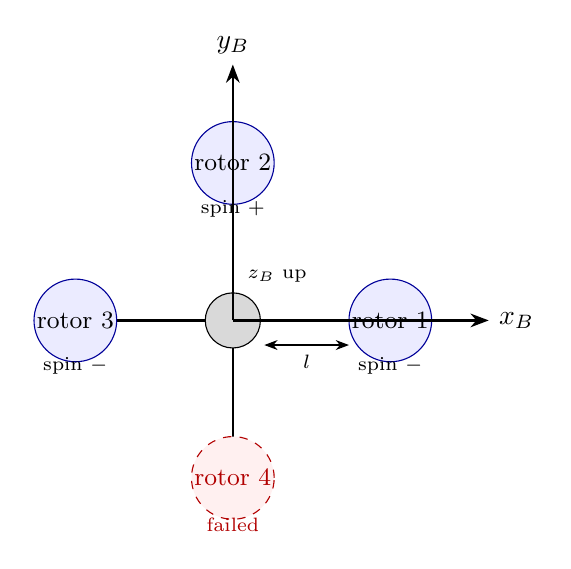
\begin{tikzpicture}[scale=1.25,>=Stealth]
  \draw[thick] (-1.6,0)--(1.6,0); \draw[thick] (0,-1.6)--(0,1.6);
  \fill[gray!30] (0,0) circle (0.28); \draw (0,0) circle (0.28);
  \foreach \p/\n/\c/\s in {(1.6,0)/1/blue/{$-$},(0,1.6)/2/blue/{$+$},(-1.6,0)/3/blue/{$-$}} {
    \draw[\c!60!black,fill=\c!8] \p circle (0.42);
    \node at \p {\small rotor \n};
    \node[below=10pt] at \p {\scriptsize spin \s};
  }
  \draw[red!70!black,fill=red!6,dashed] (0,-1.6) circle (0.42);
  \node[red!70!black] at (0,-1.6) {\small rotor 4};
  \node[red!70!black,below=11pt] at (0,-1.6) {\scriptsize failed};
  \draw[->,thick] (0,0)--(2.6,0) node[right] {$x_B$};
  \draw[->,thick] (0,0)--(0,2.6) node[above] {$y_B$};
  \node at (0.45,0.45) {\scriptsize $z_B$ up};
  \draw[<->] (0.32,-0.25)--(1.18,-0.25) node[midway,below] {\scriptsize $l$};
\end{tikzpicture}
\hspace{1.2cm}
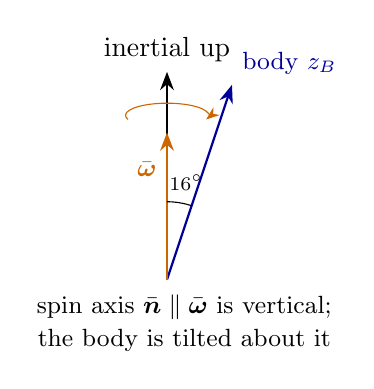
\begin{tikzpicture}[scale=1.1,>=Stealth]
  % tilted spin axis
  \draw[->,thick] (0,0)--(0,2.4) node[above] {inertial up};
  \draw[->,thick,blue!60!black] (0,0)--(0.75,2.25) node[above right] {\small body $z_B$};
  \draw[->,thick,orange!80!black] (0,0)--(0,1.7) node[left,pos=0.75] {\small $\bar{\vect\omega}$};
  \draw (0,0.9) arc (90:71.6:0.9); \node at (0.22,1.12) {\scriptsize $16^\circ$};
  \draw[->,orange!80!black] (-0.45,1.85) arc (200:-20:0.48 and 0.14);
  \node[align=center] at (0.2,-0.5) {\small spin axis $\bar{\vect n}\parallel\bar{\vect\omega}$ is vertical;\\ \small the body is tilted about it};
\end{tikzpicture}
\caption{Left: rotor layout seen from above (body frame). Rotors 1 and 3 spin with negative speed, rotor 2 with positive speed; rotor 4 has failed. Right: in the relaxed hover the drone spins about the vertical; its own $z$ axis is tilted by about 16$^\circ$ from the spin axis.}\label{fig:layout}
\end{figure}

\subsection{The state}
The simulator state has 17 numbers:
\begin{equation}
  \vect x = \big(\;\underbrace{\vect d}_{\text{position, 3}},\;\underbrace{\vect v}_{\text{velocity, 3}},\;\underbrace{\vect q}_{\text{attitude quaternion, 4}},\;\underbrace{\vect\omega=(p,q,r)}_{\text{body rates, 3}},\;\underbrace{\vect f}_{\text{motor thrusts, 4}}\;\big).
\end{equation}
Position and velocity are in the inertial frame. The body rates $p$, $q$, $r$ are the rotation rates about the body $x$, $y$ and $z$ axes (roll rate, pitch rate and yaw rate), measured in rad/s. The motor thrusts are states because a motor cannot change its thrust instantly.

\subsection{Thrust, propeller speed and the motors}
Propeller $i$ spinning at speed $\Omega_i$ (rad/s; we use $\Omega$ for propeller speeds to keep $\vect\omega$ for the body rates) produces thrust $f_i = \kappa_f\Omega_i^2$ along the body $z$ axis and a reaction torque of size $\kappa_\tau f_i$ about the same axis, with sign $(-1)^{i+1}$: rotors 1 and 3 push the body one way, rotors 2 and 4 the other way. From a thrust we recover the signed propeller speed as $\Omega_i = s_i\sqrt{f_i/\kappa_f}$ with signs $s=(-1,+1,-1,+1)$.

\paragraph{Motor lag.} Each motor follows its thrust command $u_i$ with a first-order lag of time constant $\sigma = 15$\,ms:
\begin{equation}
  \dot f_i = \frac{\operatorname{sat}(u_i) - f_i}{\sigma}.
\end{equation}
\begin{plain}
A first-order lag means that after a step change of the command, the thrust covers 63\% of the change in one time constant (15\,ms), 95\% in three time constants, and so on, like a capacitor charging.
\end{plain}

\paragraph{Saturation.} A running motor produces between $f_{\min}=0.2$\,N (idle) and $f_{\max}=3.8$\,N. Following the paper, a command $u_i\le0$ \emph{stops} the motor ($f_i=0$); this is how the spin-up strategy runs on only two rotors. A failed rotor always produces zero:
\begin{equation}
  \operatorname{sat}(u_i) = \begin{cases} 0 & u_i \le 0 \text{ or rotor $i$ failed},\\ \min(\max(u_i, f_{\min}), f_{\max}) & \text{otherwise.}\end{cases}
\end{equation}

\paragraph{Thrust loss while spinning (test plants only).} In the two-propeller flight of~\cite{mueller2014stability} the drone stayed about 2.4\,m below its set-point, which the authors attribute to the propellers producing less thrust than expected at high body rates. Our \emph{truth plants} (Section~\ref{sec:truth}) multiply every thrust by an efficiency $\eta(\vect\omega) = \max(0, 1-k\|\vect\omega\|^2)$. The nominal model, used for all designs, has $k=0$ and $\eta=1$.

\subsection{Translation: Newton's second law}
The thrust of every rotor points along the body $z$ axis, which in inertial coordinates is $R\vect e_3$. So
\begin{equation}\label{eq:trans}
  m\ddot{\vect d} = R\,\vect e_3\,\eta(\vect\omega)\,f_\Sigma - mg\,\vect e_3, \qquad f_\Sigma = \textstyle\sum_{i=1}^4 f_i .
\end{equation}
We neglect air drag on the body for translation, as the paper does.

\subsection{Rotation: Euler's equation with propellers}
The rotational dynamics are the paper's eq.~(4) with the propeller's own angular acceleration neglected:
\begin{equation}\label{eq:rot}
  I^B\dot{\vect\omega} = \vect\tau - \vect\omega\times\big(I^T\vect\omega + I^P_{zz}\,\Omega_\Sigma\,\vect e_3\big), \qquad \Omega_\Sigma = \textstyle\sum_i \Omega_i .
\end{equation}
Each term has a physical meaning:
\begin{itemize}
  \item $I^B$ is the inertia matrix of the body without propellers, and $I^T = I^B + 4I^P$ includes the propellers. Both are diagonal, with $I_{xx}=I_{yy}$ by symmetry. As in the paper, the propeller inertia about $x$ and $y$ is neglected, so $I^B_{xx} = I^T_{xx} = 3.2\times10^{-3}$\,kg\,m$^2$ and $I^B_{zz} = I^T_{zz} - 4I^P_{zz} = 5.44\times10^{-3}$\,kg\,m$^2$.
  \item $I^T\vect\omega$ is the angular momentum of the drone rotating as a rigid object.
  \item $I^P_{zz}\Omega_\Sigma\vect e_3$ is the extra angular momentum of the propellers spinning relative to the body. In normal hover the propellers cancel pairwise ($\Omega_\Sigma = 0$); after a failure they do not.
  \item $\vect\omega\times(\cdot)$ is the \emph{gyroscopic} term. When a body that carries angular momentum $\vect h$ rotates with rate $\vect\omega$, the direction of $\vect h$ changes, and that needs a torque $\vect\omega\times\vect h$. This is the same effect that makes a spinning top precess instead of falling.
\end{itemize}
The torque vector from the rotors and the yaw drag is
\begin{equation}\label{eq:torque}
  \vect\tau = \begin{pmatrix} l\,(f_2 - f_4) \\ l\,(f_3 - f_1) \\ \kappa_\tau\,(f_1 - f_2 + f_3 - f_4) - \gamma r \end{pmatrix}.
\end{equation}
The first two rows are lever arm times force: for example rotor 2 at $(0,l,0)$ pushing up with $f_2$ gives $(0,l,0)\times(0,0,f_2) = (l f_2, 0, 0)$. The third row is the sum of reaction torques minus an air-drag torque that grows linearly with the yaw rate $r$. In the truth plants every $f_i$ in~\eqref{eq:torque} is multiplied by $\eta(\vect\omega)$.

\subsection{Attitude}
We store the attitude as a \emph{unit quaternion} $\vect q = (q_w, q_x, q_y, q_z)$, four numbers with $\|\vect q\|=1$ that encode a rotation. Quaternions avoid the ``gimbal lock'' problem of Euler angles, which matters because the failed drone spins through every heading. The quaternion changes as
\begin{equation}
  \dot{\vect q} = \tfrac12\,\vect q\otimes(0,\vect\omega),
\end{equation}
where $\otimes$ is quaternion multiplication. After each integration step the quaternion is divided by its length, so that it stays a unit quaternion despite rounding errors. The rotation matrix $R(\vect q)$ is computed from it by the standard formula.

\subsection{The reduced attitude}
After the failure we give up the heading (the yaw angle), so we do not need the full attitude. We need only the direction of ``up'' as seen from the drone:
\begin{equation}
  \vect n = R^\top\vect e_3 .
\end{equation}
If the drone is level, $\vect n = (0,0,1)$; if it is upside down, $n_z<0$. Its rate of change follows from $\dot R = R[\vect\omega]_\times$ (where $[\vect\omega]_\times\vect a = \vect\omega\times\vect a$):
\begin{equation}\label{eq:ndot}
  \dot{\vect n} = \dot R^\top\vect e_3 = -[\vect\omega]_\times R^\top \vect e_3 = -\vect\omega\times\vect n .
\end{equation}
The vertical acceleration also needs only $\vect n$, because the vertical component of $R\vect e_3$ is $\vect e_3^\top R\vect e_3 = n_z$:
\begin{equation}\label{eq:vz}
  \ddot z = \frac{\eta f_\Sigma\, n_z}{m} - g .
\end{equation}
Equations~\eqref{eq:rot}, \eqref{eq:ndot} and~\eqref{eq:vz} together form a closed set in $(\vect\omega, \vect n, z, v_z)$. They do not contain the heading or the horizontal position. This is the key to the whole approach.

\subsection{The relaxed hover (spinning equilibrium)}
\paragraph{Conditions.} We look for a state in which $\vect\omega$ and $\vect n$ are constant in body coordinates and the drone neither climbs nor sinks on average:
\begin{enumerate}
  \item $\dot{\vect\omega} = 0$ in~\eqref{eq:rot}: the torques balance the gyroscopic term.
  \item $\dot{\vect n} = 0$ in~\eqref{eq:ndot}: this needs $\vect\omega\times\vect n = 0$, so the spin axis is parallel to ``up'': $\bar{\vect n} = \bar{\vect\omega}/\|\bar{\vect\omega}\|$.
  \item $\ddot z = 0$ in~\eqref{eq:vz}: $f_\Sigma\,\bar n_z = mg$.
\end{enumerate}
Condition 2 says the drone spins about the vertical. The body $z$ axis is tilted from the spin axis, so the thrust has a horizontal part of size $g\tan\theta$ per unit mass ($\theta$ is the tilt), which rotates with the spin. The centre of mass therefore moves on a small horizontal circle of radius
\begin{equation}
  \rho_{\text{orbit}} = \frac{\sqrt{1-\bar n_z^2}}{\bar n_z}\,\frac{g}{\|\bar{\vect\omega}\|^2}.
\end{equation}

\paragraph{Solving it with rotor 4 failed.} With three rotors there are more unknowns than equations, so one free choice is made. Following the paper we set $f_1 = f_3$ and $f_2 = \rho f_1$, with the design ratio $\rho = 0.5$. Then the rate equations can be solved by hand. Write $h_z = I^T_{zz}r + I^P_{zz}\Omega_\Sigma$. With $f_1=f_3$ and $f_4=0$, the torque~\eqref{eq:torque} is $(l f_2,\,0,\,\kappa_\tau(f_1-f_2+f_3)-\gamma r)$ and the gyroscopic term is
\begin{equation}
  \vect\omega\times\big(I^T\vect\omega + I^P_{zz}\Omega_\Sigma\vect e_3\big) = \Big( q\big[(I^T_{zz}-I^T_{xx})r + I^P_{zz}\Omega_\Sigma\big],\; -p\big[(I^T_{zz}-I^T_{xx})r + I^P_{zz}\Omega_\Sigma\big],\; 0 \Big).
\end{equation}
Setting $\dot{\vect\omega}=0$ row by row:
\begin{align}
  \text{row 3:}\quad & r = \kappa_\tau\,(f_1 - f_2 + f_3)/\gamma,\\
  \text{row 2:}\quad & p = 0,\\
  \text{row 1:}\quad & q = \frac{l f_2}{(I^T_{zz}-I^T_{xx})\,r + I^P_{zz}\,\Omega_\Sigma}.
\end{align}
So for any guess of $f_1$ we know all thrusts, all propeller speeds, and the rates; then $\bar{\vect n} = \vect\omega/\|\vect\omega\|$, and condition 3 becomes one equation in one unknown, $c(f_1) = f_\Sigma(f_1)\,n_z(f_1) - mg = 0$. We solve it with Brent's method, a safe root finder that needs only an interval where $c$ changes sign. The lower end of the interval is $mg/(2+\rho)$ (the thrust needed if the drone were level, $n_z = 1$).

\paragraph{Result for $\rho = 0.5$.}
\begin{center}
\small
\begin{tabularx}{\linewidth}{l l L}
\toprule
Quantity & Value & Meaning \\
\midrule
$\bar{\vect f}$ & (2.040, 1.020, 2.040, 0)\,N & rotors 1 and 3 work hardest; total 5.10\,N \\
$\bar{\vect\omega}$ & (0, 5.37, 18.81)\,rad/s, $\|\bar{\vect\omega}\| = 19.56$ & about 3.1 turns per second \\
$\bar{\vect n}$ & (0, 0.274, 0.962) & body $z$ tilted $15.9^\circ$ from vertical \\
propeller speeds & $(-564, +399, -564, 0)$\,rad/s, $\Omega_\Sigma = -729$ & propellers no longer cancel \\
orbit radius & 7.3\,mm & centre of mass nearly still \\
\bottomrule
\end{tabularx}
\end{center}
For comparison, healthy hover needs $mg/4 = 1.23$\,N per rotor.

\paragraph{Other failure cases.} With rotors 2 and 4 lost and $f_1 = f_3 = mg/2$, the drone spins about its own $z$ axis without tilt, at $r = 2\kappa_\tau f_1/\gamma = 30.1$\,rad/s. With only rotor 1 left, the thrust and all three rates must be solved together numerically; the result is $f_1 = 5.37$\,N, $\vect\omega = (14.68, 0, 32.99)$\,rad/s, $\vect n = (0.407, 0, 0.914)$. We use both cases for validation (Section~\ref{sec:validation}).

\subsection{Linear models}\label{sec:linmodels}
Control design uses linear models obtained by linearizing the nonlinear equations at an equilibrium. We build two.

\paragraph{Healthy hover (12 states, 4 inputs).} States $(x,y,z,v_x,v_y,v_z,\phi,\theta,\psi,p,q,r)$, where $\phi,\theta,\psi$ are roll, pitch and yaw angles (Euler angles in the order yaw, pitch, roll); inputs are the four thrusts, trimmed at $mg/4$. Euler angles are fine here because the healthy drone stays near level. The open-loop eigenvalues are eleven zeros and $-0.506$\,s$^{-1}$ (the yaw-drag mode, $-\gamma/I^B_{zz}$). Near hover, positions, velocities, angles and the roll and pitch rates all act as integrators; the repeated zeros form chains of integrators, so the open loop is unstable.

\paragraph{Failed drone (7 states, 3 inputs).} States $\vect s = (p, q, r, n_x, n_y, z, v_z)$ and inputs $(f_1, f_2, f_3)$. Only $n_x$ and $n_y$ are states, because $n_z = \sqrt{1-n_x^2-n_y^2}$ follows from them. Because equations~\eqref{eq:rot}, \eqref{eq:ndot} and~\eqref{eq:vz} do not depend on the heading or on time, \textbf{the linearization about the relaxed hover is time invariant}, even though the drone is spinning in the inertial frame. (In inertial coordinates the spinning equilibrium would be a periodic orbit, and one would need Floquet theory, the stability theory of linear systems with periodic coefficients.) The numerical Jacobians at $\rho=0.5$ are
\begin{equation}
A = \begin{pmatrix}
 0 & -10.10 & -3.86 & 0 & 0 & 0 & 0\\
 10.10 & 0 & 0 & 0 & 0 & 0 & 0\\
 0 & 0 & -0.51 & 0 & 0 & 0 & 0\\
 0 & -0.96 & 0.27 & 0 & 20.34 & 0 & 0\\
 0.96 & 0 & 0 & -18.81 & 0 & 0 & 0\\
 0 & 0 & 0 & 0 & 0 & 0 & 1\\
 0 & 0 & 0 & 0 & -2.91 & 0 & 0
\end{pmatrix},\qquad
B = \begin{pmatrix}
 3.48 & 48.21 & 3.48\\
 -53.13 & 0 & 53.13\\
 3.11 & -3.11 & 3.11\\
 0 & 0 & 0\\ 0 & 0 & 0\\ 0 & 0 & 0\\
 1.92 & 1.92 & 1.92
\end{pmatrix}.
\end{equation}
Every entry can be traced to the physics:
\begin{itemize}
  \item $A_{pq} = -A_{qp} = \bar a = \frac{I^T_{xx}-I^T_{zz}}{I^B_{xx}}\bar r - \frac{I^P_{zz}}{I^B_{xx}}\bar\Omega_\Sigma = -10.10$: the gyroscopic coupling between roll and pitch rate (the paper's eq.~28).
  \item $A_{pr} = -\bar q(I^T_{zz}-I^T_{xx})/I^B_{xx} = -3.86$: a change of yaw rate changes the gyroscopic roll torque.
  \item $A_{rr} = -\gamma/I^B_{zz} = -0.51$: yaw drag.
  \item The $\vect n$ rows are the linearization of $\dot{\vect n} = -\vect\omega\times\vect n$. The coefficient of $n_y$ in $\dot n_x$ is $\bar r + \bar q\bar n_y/\bar n_z = 20.34$, because $n_z$ changes with $n_y$. The paper's simplified matrix (its eq.~27) uses $\bar r = 18.81$ there; we use the exact Jacobian.
  \item $A_{v_z n_y} = -\bar f_\Sigma\bar n_y/(m\bar n_z) = -2.91$: tilting the thrust away from vertical reduces the vertical force. This entry exists only because the equilibrium is tilted.
  \item $B_{p,f_2} = l/I^B_{xx} = 53.13$ minus a gyroscopic correction (changing $f_2$ changes propeller 2's speed and so $\Omega_\Sigma$), giving 48.21. The same correction gives the small entries 3.48 for $f_1$ and $f_3$.
  \item $B_{v_z,f_i} = \bar n_z/m = 1.92$: more thrust, more vertical acceleration.
\end{itemize}
The eigenvalues of $A$ are $\pm10.10j$ (the $p$--$q$ gyroscopic oscillation), $\pm19.56j$ (the tilt of the spin axis seen from the spinning body; its frequency equals $\|\bar{\vect\omega}\|$), $-0.51$ (yaw drag) and a double zero (altitude: height is the integral of vertical speed, which is the integral of the vertical force). No eigenvalue has a positive real part, but the open loop is not stable: the two oscillations are undamped and the altitude double integrator drifts (its height error grows linearly). Feedback is needed.

\paragraph{Adding the motors.} The motors are added as three more states with $\dot{\vect f} = (\vect u - \vect f)/\sigma$; the thrusts in $B$ then act through these states. This gives the 10-state model used by the failure LQR, the MPC and the certificate.

\subsection{Truth plants for learning}\label{sec:truth}
If we generated learning data with the same model that the controller uses, a learned correction would have nothing to learn, and any improvement would be an artefact. We therefore generate data from \emph{truth plants} that contain effects the nominal model lacks (Table~\ref{tab:params}). Family A is used for training, family B (different magnitudes, in different directions) only for testing. A third, randomized family draws new values for every training episode; its ranges cover A but not B.

\begin{table}[h]
\centering\small
\caption{Nominal parameters~\cite{mueller2014stability} and truth-plant families. $k$ is the thrust-loss coefficient in $\eta = 1-k\|\vect\omega\|^2$.}\label{tab:params}
\begin{tabularx}{\linewidth}{l l L}
\toprule
Quantity & Symbol & Value \\
\midrule
Mass, arm length & $m$, $l$ & 0.50\,kg, 0.17\,m \\
Total inertia & $I^T_{xx}$, $I^T_{zz}$ & $3.2$, $5.5\times10^{-3}$\,kg\,m$^2$ \\
Propeller inertia & $I^P_{zz}$ & $1.5\times10^{-5}$\,kg\,m$^2$ \\
Thrust coefficient & $\kappa_f$ & $6.41\times10^{-6}$\,N\,s$^2$/rad$^2$ \\
Torque-to-thrust ratio & $\kappa_\tau$ & 0.0169\,m \\
Yaw drag & $\gamma$ & $2.75\times10^{-3}$\,N\,m\,s/rad \\
Thrust range, motor lag & $[f_{\min},f_{\max}]$, $\sigma$ & [0.2, 3.8]\,N, 15\,ms \\
\midrule
Family A (training) & & $k=1.5\times10^{-4}$\,s$^2$/rad$^2$, $I_{xx}\times1.08$, $I_{zz}\times0.95$, $\sigma=20$\,ms \\
Family B (held out) & & $k=2.5\times10^{-4}$\,s$^2$/rad$^2$, $I_{xx}\times0.94$, $I_{zz}\times1.06$, $\sigma=12$\,ms \\
Randomized & & $k\in[0, 2\times10^{-4}]$, $I_{xx}\times[0.96,1.10]$, $I_{zz}\times[0.93,1.03]$, $\sigma\in[15,22]$\,ms \\
\bottomrule
\end{tabularx}
\end{table}
At the relaxed hover ($\|\vect\omega\|\approx19.6$\,rad/s), family A loses about 6\% of its thrust and family B about 10\%.

%=====================================================================
\section{How the model is coded}\label{sec:code}
%=====================================================================
All code is our own and written in Python 3.12 with NumPy~\cite{harris2020numpy} and SciPy~\cite{virtanen2020scipy}. It lives in a small package, \texttt{rotorfail/}, plus one script per experiment in \texttt{experiments/} and automated tests in \texttt{tests/}. This section walks through the parts that implement Section~\ref{sec:model}. The listings are excerpts of the real code, shortened for reading (options such as the motor-lag switch, solver fallbacks and iteration limits are left out).

\subsection{Package layout}
\begin{table}[h]
\centering\small
\begin{tabularx}{\linewidth}{l L}
\toprule
Module & What it contains \\
\midrule
\texttt{params.py} & All vehicle parameters in one frozen data class \texttt{QuadParams}; the truth-plant families \\
\texttt{dynamics.py} & The 17-entry state layout, quaternion helpers, saturation, the equations of motion, one RK4 step \\
\texttt{sim.py} & The simulation loop with a sampled (zero-order-hold) controller \\
\texttt{equilibrium.py} & Solvers for the relaxed hover (one, two and three rotors lost) \\
\texttt{models.py} & The healthy and failed nonlinear models in design coordinates; numerical Jacobians; motor-lag augmentation \\
\texttt{analysis.py} & Controllability and observability tests, Gramians, delay margin \\
\texttt{control.py} & Healthy LQR, failure LQR, spin-up strategy, detection-delay supervisor \\
\texttt{metrics.py} & The success criterion, fixed before the experiments \\
\texttt{koopman.py} & Data generation, dictionary, full-state and residual EDMDc, error evaluation \\
\texttt{mpc.py} & Linear MPC with an optional learned residual \\
\texttt{certify.py} & LMI certificate (saturation-aware invariant ellipsoid) \\
\texttt{validation.py} & Independent implementation of the IJRR 2016 model, used only for validation \\
\bottomrule
\end{tabularx}
\end{table}

\subsection{Parameters}
\texttt{QuadParams} is a frozen data class: once created, its values cannot change by accident. Derived quantities are computed properties, for example $I^B_{xx} = I^T_{xx} - 4I^P_{xx}$ and the torque vector~\eqref{eq:torque}:
\begin{lstlisting}
@dataclass(frozen=True)
class QuadParams:
    m: float = 0.50              # kg
    l: float = 0.17              # m, arm length
    Ixx_T: float = 3.2e-3        # total inertia about x and y
    ...
    thrust_loss: float = 0.0     # truth-plant effect k (0 in the nominal model)
    prop_sign: tuple = (-1.0, 1.0, -1.0, 1.0)

    def body_torque(self, f, r):
        f1, f2, f3, f4 = f
        return np.array([self.l * (f2 - f4),
                         self.l * (f3 - f1),
                         self.kappa_tau * (f1 - f2 + f3 - f4) - self.gamma * r])
\end{lstlisting}
A truth plant is created with \texttt{dataclasses.replace}, which copies the nominal parameters and changes only some of them, for example family A: \texttt{replace(base, thrust\_loss=1.5e-4, Ixx\_T=base.Ixx\_T*1.08, ...)}.

\subsection{Equations of motion}
\texttt{deriv(x, f\_cmd, p, alive)} returns $\dot{\vect x}$ for the 17-entry state. It is a direct transcription of equations~\eqref{eq:trans} to~\eqref{eq:torque}:
\begin{lstlisting}
def body_rate_derivative(w, f, p):
    w_sigma = np.sum(p.prop_speeds(f))                    # sum of signed propeller speeds
    h = p.I_T @ w + p.Izz_P * w_sigma * E3                # angular momentum
    tau = p.body_torque(f * p.thrust_efficiency(w), w[2])
    return np.linalg.solve(p.I_B, tau - np.cross(w, h))   # eq. (rot)

def deriv(x, f_cmd, p, alive, motor_lag=True):
    q, w = x[IDX_Q], x[IDX_W]
    f_sat = saturate(f_cmd, p, alive)                     # 0 if stopped/failed, else clipped
    f = np.where(alive, x[IDX_F], 0.0)
    f_dot = np.where(alive, (f_sat - f) / p.sigma_mot, 0.0)   # motor lag
    R = quat_to_rot(q)
    acc = R @ E3 * np.sum(f) * p.thrust_efficiency(w) / p.m - G * E3
    q_dot = 0.5 * quat_mult(q, np.concatenate(([0.0], w)))
    w_dot = body_rate_derivative(w, f, p)
    return np.concatenate((x[IDX_V], acc, q_dot, w_dot, f_dot))
\end{lstlisting}
The boolean vector \texttt{alive} says which rotors work; a failed rotor's thrust is forced to zero. The same function \texttt{body\_rate\_derivative} is used by the simulator, by the equilibrium solver and by the linear models, so they cannot disagree with each other.

\subsection{Integration and the sampled controller}
\texttt{rk4\_step} performs one classical Runge--Kutta step and then renormalizes the quaternion:
\begin{lstlisting}
def rk4_step(x, f_cmd, dt, p, alive):
    k1 = deriv(x, f_cmd, p, alive)
    k2 = deriv(x + 0.5 * dt * k1, f_cmd, p, alive)
    k3 = deriv(x + 0.5 * dt * k2, f_cmd, p, alive)
    k4 = deriv(x + dt * k3, f_cmd, p, alive)
    x_new = x + dt / 6.0 * (k1 + 2 * k2 + 2 * k3 + k4)
    x_new[IDX_Q] /= np.linalg.norm(x_new[IDX_Q])
    return x_new
\end{lstlisting}
\texttt{simulate} runs the loop. The plant is integrated with step $\Delta t$ (0.5 to 1\,ms), but the controller is called only once per control period (1 to 5\,ms) and its command is held constant in between. This is exactly a digital controller with a zero-order hold:
\begin{lstlisting}
for k in range(n_steps + 1):
    t = k * dt
    if k % ctrl_every == 0:
        u = controller(t, x)          # sampled controller, held between calls
    ...                               # logging, optional early stop
    x = rk4_step(x, u, dt, p, alive_fn(t), motor_lag)
\end{lstlisting}
Every controller is a Python object called as \texttt{controller(t, x)} that returns four thrust commands. Controllers that keep internal state (filters, mode flags) provide a \texttt{reset} method. A supervisor may provide \texttt{alive(t)} to say when the rotor fails.

\subsection{Equilibrium solver}
\texttt{relaxed\_hover(p, rho)} implements Section~\ref{sec:model}: a closed-form function for the rates and a one-dimensional root search for $f_1$:
\begin{lstlisting}
def relaxed_hover(p, rho=0.5):
    def residual(f1):
        f = np.array([f1, rho * f1, f1, 0.0])
        w = _rates_for_thrust(f, p, w_guess)          # p = 0, r and q in closed form
        n = w / np.linalg.norm(w) * np.sign(w[2])
        return np.sum(f) * p.thrust_efficiency(w) * n[2] - p.weight
    f_lo = p.weight / (2 + rho)                       # thrust if the drone were level
    f1 = brentq(residual, f_lo * (1 + 1e-9), 6 * f_lo, xtol=1e-14)
    ...
\end{lstlisting}
When thrust loss is switched on, or the thrusts do not satisfy $f_1 = f_3$ and $f_4 = 0$, the closed form no longer applies, and \texttt{\_rates\_for\_thrust} falls back to SciPy's \texttt{fsolve} on $\dot{\vect\omega}=0$.

\subsection{Linear models}
The linear models are not typed in by hand. \texttt{failed\_f} writes the 7-state equations, reusing \texttt{body\_rate\_derivative}, and \texttt{jacobians} differentiates them numerically by central differences with $\epsilon = 10^{-6}$:
\begin{lstlisting}
def failed_f(s, u3, p):
    w, nx, ny = s[0:3], s[3], s[4]
    nz = np.sqrt(max(1.0 - nx * nx - ny * ny, 1e-12))
    n = np.array([nx, ny, nz])
    f = np.array([u3[0], u3[1], u3[2], 0.0])
    w_dot = body_rate_derivative(w, f, p)
    n_dot = -np.cross(w, n)
    vz_dot = np.sum(f) * nz / p.m - G
    return np.array([*w_dot, n_dot[0], n_dot[1], s[6], vz_dot])

def jacobians(fun, x0, u0, eps=1e-6):
    for i in range(n):          # A[:, i] = (f(x0 + e_i eps) - f(x0 - e_i eps)) / (2 eps)
        ...
\end{lstlisting}
This avoids transcription errors, and the tests check the result against finite differences of the same nonlinear function and against the paper's closed-form entries (for example $\bar a$). \texttt{add\_motor\_lag} then appends the three motor states.

\subsection{Reproducibility}
Every random number comes from \texttt{numpy.random.default\_rng(seed)} with a fixed seed written in the experiment script. Every table and figure in this report is written by one script in \texttt{experiments/}. Success criteria are written in code (\texttt{metrics.py}) before the experiments are run, so they cannot be tuned afterwards. Appendix~\ref{app:repro} lists the commands.

%=====================================================================
\section{How we validated the simulator}\label{sec:validation}
%=====================================================================
Every later result depends on the simulator, so before using it we checked it in three independent ways:
\begin{enumerate}
  \item \textbf{Physics tests}: compare the simulator with results derived by hand (exact formulas, conservation laws). These catch coding errors.
  \item \textbf{Published numbers}: compare with the numbers printed in three papers. These catch modelling errors (a wrong sign, a missing term, a wrong parameter).
  \item \textbf{Flight data}: compare with measurements from a real flight. This tells us how close the \emph{model itself} is to reality.
\end{enumerate}
All checks are automated tests that run with one command (\texttt{pytest}). At the time of writing, 46 tests pass and 1 is marked as an expected failure (explained in Section~\ref{sec:val-icra}). A script in the \texttt{experiments} folder (\texttt{v0\_validation\_report.py}) also writes all comparisons into one table in \texttt{results/tables}.

\subsection{Layer 1: physics tests against hand-derived results}
Each test sets up a situation whose answer is known exactly, runs the simulator and compares. None of them compares the simulator with another run of itself.
\begin{longtable}{p{0.27\linewidth}p{0.66\linewidth}}
\toprule
Test & Exact reference result \\
\midrule
\endhead
Free fall & With no thrust: $z(t) = z_0 + v_{z0}t - \tfrac12 gt^2$, and horizontal motion at constant speed (agreement to $10^{-9}$). \\
Thrust direction & Tilted drone, no torque: $\ddot{\vect d} = R\vect e_3 f_\Sigma/m - g\vect e_3$, with $R$ built by hand from Euler angles. \\
Hover balance & With $f_i = mg/4$ all derivatives are zero. \\
Torque-free precession & No thrust, no drag: $r$ stays constant and $(p,q)$ rotate at the rate $\lambda = (I^T_{zz}-I^T_{xx})r/I^B_{xx}$ (Euler's equations solved in closed form; agreement to $10^{-8}$). \\
Angular momentum and energy & For a torque-free rigid body the inertial angular momentum $R I\vect\omega$ and the kinetic energy $\tfrac12\vect\omega^\top I\vect\omega$ must stay constant (relative error below $10^{-8}$). \\
Reduced-attitude kinematics & For constant $\vect\omega$: $\vect n(t) = e^{-[\vect\omega]_\times t}\vect n(0)$, computed with the matrix exponential. \\
Yaw spin-up & Rotors 1 and 3 only, equal thrust: $p=q=0$ stay zero and $I^B_{zz}\dot r = 2\kappa_\tau f - \gamma r$, so $r(t) = r_{ss}(1-e^{-\gamma t/I^B_{zz}})$ with $r_{ss} = 2\kappa_\tau f/\gamma$. \\
Integration order & Halving the time step must reduce the error by about $2^4 = 16$ (RK4 is fourth order); the test accepts 12 to 20. \\
Motor lag & Step response $f(t) = u + (f_0 - u)e^{-t/\sigma}$. \\
Saturation rules & Command $\le0$ gives 0; otherwise clipped to $[f_{\min}, f_{\max}]$; a failed rotor gives 0. \\
Paper's equations & An independent transcription of the paper's eqs.~(12) to (14), written with signed propeller speeds instead of thrusts, equals the simulator at 50 random states. \\
IJRR model reduces to ours & Our separate implementation of the IJRR 2016 model (Section~\ref{sec:val-ijrr}), with its extra effects switched off, equals the simulator at 50 random states. \\
Centre-of-mass motion & At the relaxed hover the vertical acceleration is zero and the horizontal acceleration is $g\sqrt{1-n_z^2}/n_z$ (the paper's eqs.~18 to 20). \\
\bottomrule
\end{longtable}

\subsection{Layer 2: published numbers}
\subsubsection{Mueller and D'Andrea, ICRA 2014}\label{sec:val-icra}
This paper uses exactly our model and parameters, so we expect exact agreement up to the digits printed.
\begin{table}[h]
\centering\small
\caption{Our equilibria against Mueller and D'Andrea, ICRA 2014.}\label{tab:val-icra}
\setlength{\tabcolsep}{4pt}
\begin{tabularx}{\linewidth}{>{\raggedright\arraybackslash}p{3.1cm} L r r r}
\toprule
Case & Quantity & Ours & Published & Difference \\
\midrule
Two opposing rotors lost (eqs.~57--59) & $f_1 = f_3$ (N) & 2.453 & 2.45 & +0.10\% \\
 & propeller speed $\Omega_1$ (rad/s) & $-618.6$ & $-619$ & +0.07\% \\
 & $r$ (rad/s) & 30.14 & 30.1 & +0.14\% \\
\midrule
Three rotors lost (eqs.~62--64) & $f_1$ (N) & 5.369 & 5.37 & $-0.02$\% \\
 & propeller speed $\Omega_1$ (rad/s) & $-915.2$ & $-915$ & $-0.02$\% \\
 & $(p, q, r)$ (rad/s) & (14.68, 0, 32.99) & (14.7, 0, 33.0) & $\le0.11$\% \\
 & $\vect n$ & (0.407, 0, 0.914) & (0.41, 0, 0.91) & $\le0.8$\% \\
\midrule
One rotor lost, $\rho = 0.5$ (eqs.~50--53) & $f_1 = f_3$, $f_2$ (N) & 2.040, 1.020 & 2.05, 1.02 & $-0.5$\%, 0\% \\
 & $r$ (rad/s) & 18.81 & 18.89 & $-0.4$\% \\
 & $n_z$ & 0.962 & 0.958 & +0.4\% \\
 & $q$ (rad/s) & 5.37 & 5.69 & $-5.7$\% \\
 & $n_y$ & 0.274 & 0.289 & $-5.1$\% \\
\midrule
Fig.~3 ($\rho$ sweep) & min $\|\vect\omega\|$ (rad/s) at $\rho$ & 18.62 at 0.675 & 19.0 at 0.655 & $-2.0$\%, +3.0\% \\
 & min $f_1$ (N) at $\rho$ & 2.029 at 0.579 & 2.04 at 0.563 & $-0.5$\%, +2.8\% \\
\bottomrule
\end{tabularx}
\end{table}

\paragraph{Reading.} The two-rotor and three-rotor cases agree to every printed digit. The three-rotor case is a strong check because it exercises all gyroscopic and propeller terms with $p\ne0$. In the one-rotor case the thrusts, the yaw rate and $n_z$ agree within 0.5\%, but $q$ and $n_y$ are 6\% lower. We investigated this gap:
\begin{itemize}
  \item Inserting the paper's own published values ($\vect f$, $\vect\omega$) into the paper's own roll equation (its eq.~12) does \emph{not} give zero: it leaves a roll torque of $-0.011$\,N\,m, about 7\% of the torque from rotor 2. So the published one-rotor values are not an exact equilibrium of the paper's own model with its stated parameters.
  \item The published inertias have only two significant figures. Changing each by $\pm0.05\times10^{-3}$ moves our $q$ between 5.07 and 5.69\,rad/s, so the published value lies at the edge of what rounding allows; but the same parameters reproduce the other two cases exactly.
\end{itemize}
We therefore treat this as an inconsistency in that one published case, not as an error in our model. The test for the published $q$ is kept and marked as an expected failure, so the discrepancy stays visible.

\paragraph{Analytic checks.} The paper's closed form for the yaw rate (its eq.~21) equals our solver. Its coupling constant $\bar a$ (eq.~28) equals the $(p,q)$ entry of our numerical Jacobian. Its controllability condition (eqs.~37 to 39) says that with two opposing rotors lost, the roll rate becomes uncontrollable exactly when $\bar a = 0$; our controllability rank drops from 7 to 6 exactly there.

The sweep over the thrust ratio $\rho$ (Figure~\ref{fig:rho}) reproduces the shape of the paper's Fig.~3; the minima agree within 2\% in value and 3\% in location. Both minima are shallow, so their location is sensitive to small differences.

\begin{figure}[h]
\centering
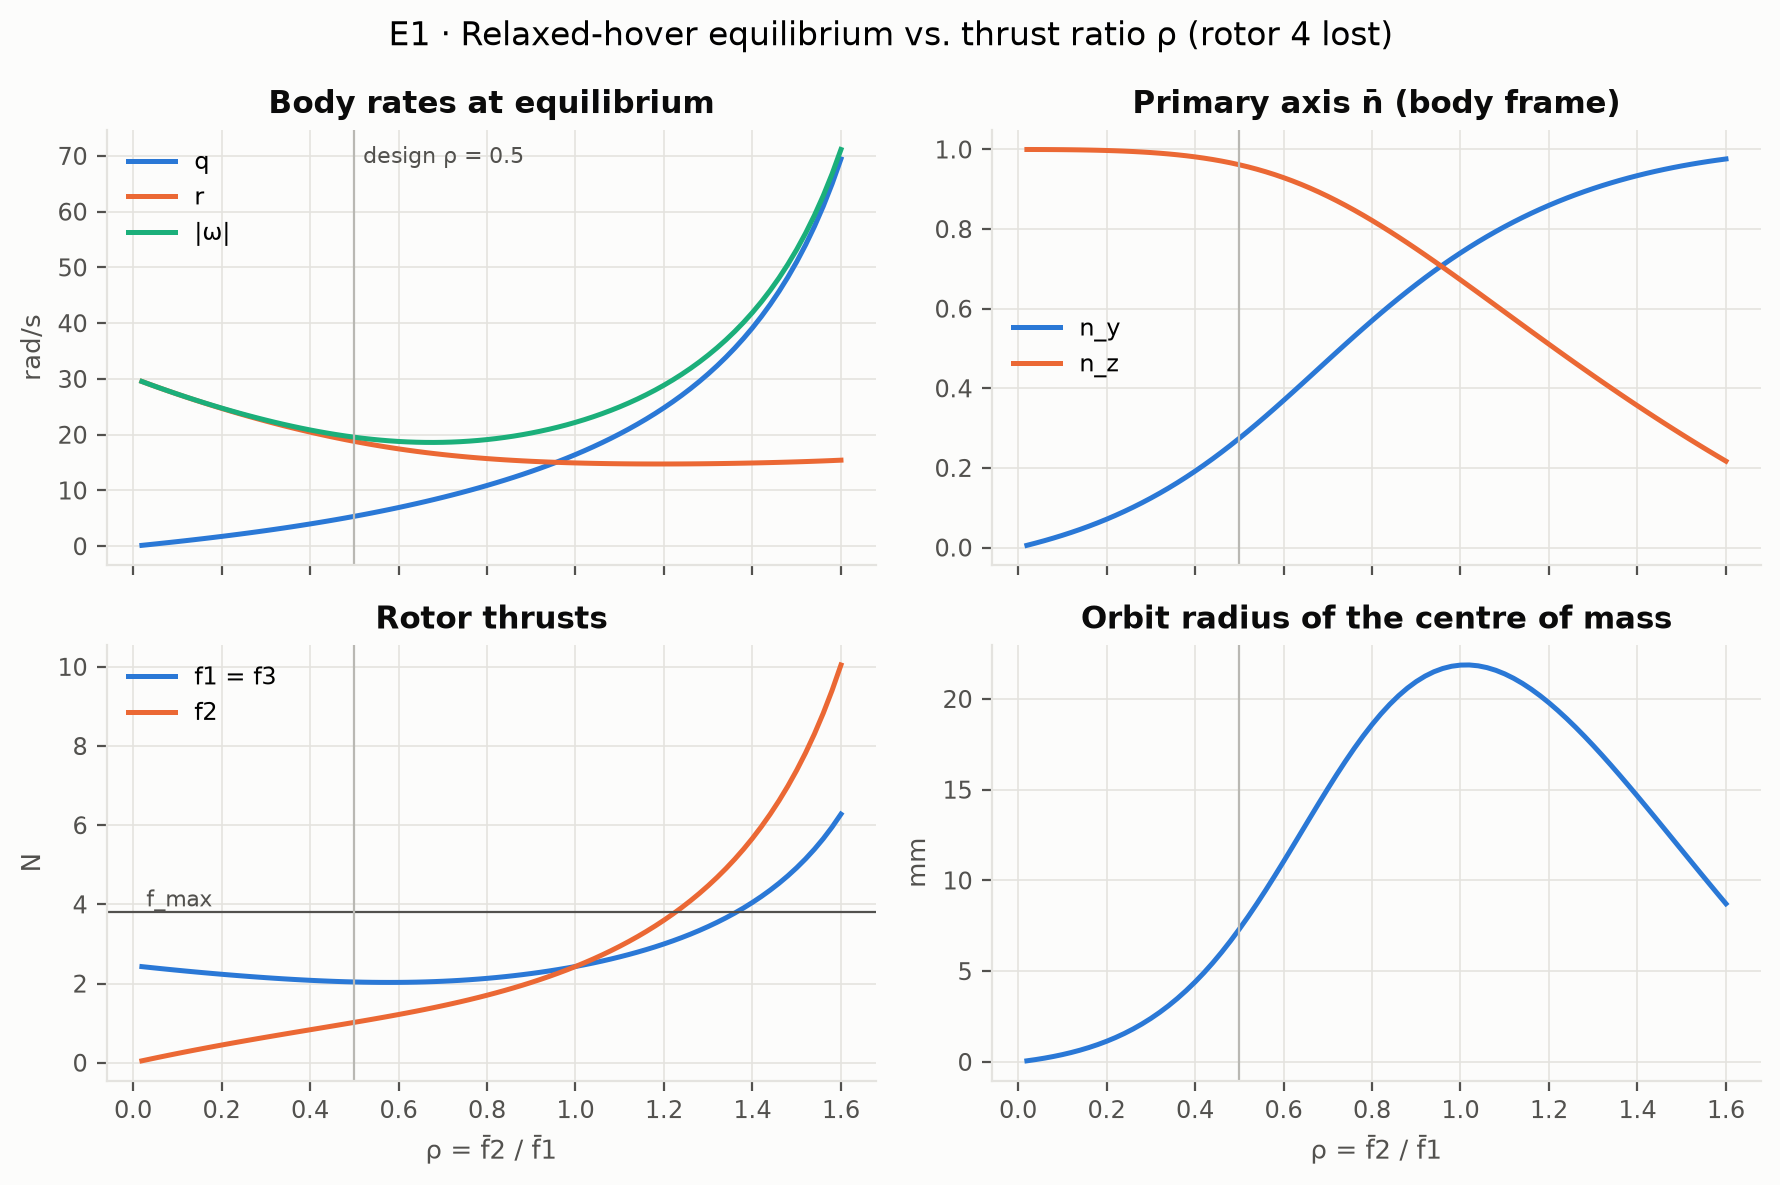
\includegraphics[width=0.85\linewidth]{figures/e1_rho_sweep.png}
\caption{The one-rotor-loss equilibrium as a function of the thrust ratio $\rho = f_2/f_1$ (reproduces the paper's Fig.~3).}\label{fig:rho}
\end{figure}

\subsubsection{Mueller and D'Andrea, IJRR 2016}\label{sec:val-ijrr}
This paper uses the same drone with a more detailed model (air-relative thrust, quadratic drag on all axes, propeller speeds as inputs, the propeller acceleration term kept). To check it we wrote a \emph{separate} implementation, \texttt{validation.py}, deliberately in different variables (propeller speeds instead of thrusts), so that it does not share code with the simulator. For each of the five published cases we give it the published propeller speeds and solve for the body rates at which the rotation stops changing.

\begin{table}[h]
\centering\small
\caption{Hover solutions of IJRR 2016 (Sec.~5.2) against our independent implementation. The last column is $f_\Sigma n_z/(mg)$, which must be 1 at a hover solution.}\label{tab:val-ijrr}
\begin{tabular}{lllll}
\toprule
Case & Published $\Omega$ (rad/s) & Published $\vect\omega$ & Ours & Force ratio \\
\midrule
No failure & (438, 438, 438, 438) & (0, 0, 0) & (0, 0, 0) & 1.003 \\
Rotor 4 lost & (585, 362, 585, 0) & (0.20, 4.30, 19.50) & (0.15, 4.19, 19.47) & 1.002 \\
Rotors 2, 4 lost & (643, 0, 643, 0) & (0, 0, 24.50) & (0, 0, 24.50) & 1.001 \\
Rotors 3, 4 lost & (1067, 218, 0, 0) & (26.00, 0, 23.30) & (24.94, 0.06, 23.57) & 0.995 \\
Rotors 2, 3, 4 lost & (1103, 0, 0, 0) & (28.00, $-1.60$, 24.50) & (26.73, $-1.45$, 24.93) & 0.994 \\
\bottomrule
\end{tabular}
\end{table}

\paragraph{Reading.} With the published parameters, the body-rate vectors agree within 4\% and the force balance within 0.6\%. The two cases with very high rotation rates are the most sensitive to the drag and inertia values, which are printed with one or two significant figures. As a sensitivity check only, $I_{xx} = 2.75\times10^{-3}$ (the upper end of the rounding interval of the printed $2.7\times10^{-3}$) brings all five cases within 0.7\%; because this value was chosen by looking at the same cases, it is not an independent validation.

One number is especially informative. With two opposing rotors lost, the paper's propeller speed is 643\,rad/s at a body spin of 24.5\,rad/s. If thrust depended on the speed relative to the body, $\kappa_f\cdot643^2$ would be 8\% more than $mg/2$; with the speed relative to the air, $\kappa_f(643-24.5)^2 = mg/2$ exactly. So air-relative thrust is real and matters. Our simulator (the ICRA model) does not include it: at the one-rotor equilibrium it would change rotors 1 and 3 by about $-7$\% and rotor 2 by about $+10$\%. This is a known limitation (Section~\ref{sec:discussion}).

\subsubsection{Sun et al., T-RO 2021: a second airframe}
To test the equilibrium solver on a different drone, we used the Parrot Bebop~2 parameters of Sun et al.~\cite{sun2020incremental} (their Table~I in the arXiv version, called Table~III in their text: $m=0.410$\,kg, $l=0.145$\,m, and so on). With two opposing rotors lost, their eq.~(60) gives $\bar r = mg\kappa_\tau/\gamma$ and propeller speed $\sqrt{mg/(2\kappa_f)}$.

\begin{center}\small
\begin{tabular}{lrrr}
\toprule
Quantity & Ours & Eq.~(60) with the parameter table & Printed in the text \\
\midrule
$\bar r$ (rad/s) & 26.81 & 26.81 & 26.4 \\
propeller speed (rad/s) & 1029 & 1029 & 1015 \\
\bottomrule
\end{tabular}
\end{center}
Our solver equals the paper's own formula exactly. The numbers printed in the paper's text are about 1.5\% below its own formula; this difference is internal to the paper.

\subsection{Layer 3: flight data}
\paragraph{Spin-up time.} In the ICRA flight (their Fig.~4), propeller 4 is switched off and the drone flies on propellers 1 and 3 only, without attitude feedback, until the rotation rate reaches 10\,rad/s, which took 0.62\,s. During this phase the roll and pitch torques are zero (rotors 1 and 3 are opposite each other with equal thrust), so only the yaw equation acts:
\begin{equation}
  I^B_{zz}\dot r = 2\kappa_\tau f - \gamma r \quad\Rightarrow\quad r(t) = r_{ss}\big(1 - e^{-\gamma t/I^B_{zz}}\big),\quad r_{ss} = \frac{2\kappa_\tau f}{\gamma},
\end{equation}
so the time to reach 10\,rad/s is $t_{10} = -\frac{I^B_{zz}}{\gamma}\ln\!\big(1 - \tfrac{10}{r_{ss}}\big)$. The answer depends strongly on the thrust $f$ of the two rotors. The paper's text says only that the vehicle ``uses only the two opposing propellers'' during this phase; the thrust is not printed, so we read it from its Fig.~4: rotor 2 is at zero and rotors 1 and 3 at a constant 2.95\,N or so (more than $mg/2 = 2.45$\,N).

\begin{center}\small
\begin{tabular}{lccc}
\toprule
Spin-up thrust & Simulator & Closed form & Flight \\
\midrule
2.95\,N (read from Fig.~4) & 0.65\,s & 0.64\,s & 0.62\,s \\
2.45\,N ($mg/2$) & 0.81\,s & 0.80\,s & not flown \\
\bottomrule
\end{tabular}
\end{center}
At the flight thrust the model is within about 4\% of the flight. Because the thrust is read from a plot, the detection-delay study (Section~\ref{sec:delay}) is reported for both thrusts.

\paragraph{Steady spin rate and height.} The published models over-predict the spin of the real drone. In the ICRA one-rotor flight the measured body rates in hover were $(2.1, 3.7, 13.7)$\,rad/s (their eq.~55), about 14.3\,rad/s against about 19.7\,rad/s predicted by the same model that our simulator implements (ours: 19.6\,rad/s at $\rho = 0.5$), about 27\% less. In the IJRR flight the spin was 15.8\,rad/s against 19.9\,rad/s in simulation (their Sec.~5.4), about 20\% less; those authors suggest extra torques from the motion of the propeller centres as a possible cause. In the ICRA two-rotor flight the drone stayed about 2.4\,m below its set-point, which the authors attribute to the propellers producing less thrust at high body rates. None of these effects is in the nominal model. They are why our truth plants contain a thrust loss at high rotation rate: the learned residual of Section~\ref{sec:koopman} is meant to capture effects of this kind.

\subsection{Summary of the validation}
\begin{plain}
The simulator agrees with the papers wherever the papers are internally consistent, and the only disagreements are explained: one published case that does not satisfy the paper's own equation, two cases whose parameters are printed with very few digits, and two real-world effects (air-relative thrust and thrust loss while spinning) that the paper's own model also leaves out. We can therefore trust the simulator as a faithful implementation of the published model, and we know in which ways the published model differs from the real drone.
\end{plain}

%=====================================================================
\section{Linear analysis and LQR controllers}\label{sec:linear}
%=====================================================================
\subsection{Controllability: can three rotors steer the failed drone?}
\paragraph{Method.} For both linear models we computed three things (experiment E2, \texttt{analysis.py}):
\begin{enumerate}
  \item The rank of the controllability matrix $\mathcal C = [B, AB, \dots, A^{n-1}B]$. Its columns differ in size by many orders of magnitude (each multiplication by $A$ scales them by about 20), which can make a numerical rank test unreliable. We therefore divide every column by its length before computing the singular values (``scaled rank'').
  \item The PBH test for every eigenvalue $\lambda$ of $A$: the smallest singular value of $[\lambda I - A,\; \tilde B]$, where $\tilde B$ is $B$ rescaled to the size of $A$. A value near zero would mark an uncontrollable mode.
  \item The controllability Gramian over 1\,s, $W_c(T) = \int_0^T e^{As}BB^\top e^{A^\top s}ds$. It is computed exactly with Van Loan's method: the matrix exponential of the block matrix $\begin{psmallmatrix}-A & BB^\top\\ 0 & A^\top\end{psmallmatrix}T$ contains $W_c$ in its blocks. This works even for the undamped modes, where the infinite-time Gramian does not exist.
\end{enumerate}

\paragraph{Result.} Both models are controllable. The failed model has rank 7 of 7, and every mode passes the PBH test (smallest values between 0.016 and 0.28, none near zero). The Gramian's smallest eigenvalue is 0.54 and its condition number $7.6\times10^3$: some directions need much more effort than others, but none is out of reach. This reproduces the paper's controllability result; it is not a new finding.

\subsection{Observability: what can the sensors see?}
\paragraph{Method.} A controller needs the state, so we asked which sensors make it observable. For each sensor set we built the output matrix $C$, checked the rank of the observability matrix, and computed the 1\,s observability Gramian. Different sensors measure different units with different noise, so before computing the Gramian we divided each output by an assumed noise level (one standard deviation): gyroscope 0.005\,rad/s, position 0.01\,m, attitude 0.01\,rad, magnetometer heading 0.02\,rad, tilt estimate 0.01, barometer 0.1\,m. The Gramian is then dimensionless, and its smallest eigenvalue says how well the weakest direction is seen \emph{relative to the noise}.

\begin{table}[h]
\centering\small
\caption{Observability of the failed drone's linear model (7 states) for four sensor sets.}\label{tab:obs}
\begin{tabular}{lccc}
\toprule
Sensors & Rank & Cannot see & Smallest eigenvalue of $W_o(1\,\mathrm{s})$ \\
\midrule
Gyroscope $(p,q,r)$ & 3/7 & $n_x, n_y, z, v_z$ & 0 \\
Gyroscope + tilt estimate $(n_x, n_y)$ & 5/7 & $z, v_z$ & 0 \\
Gyroscope + barometer $(z)$ & 7/7 & nothing & $2.4\times10^{-3}$ \\
Gyroscope + tilt + barometer & 7/7 & nothing & 6.6 \\
\bottomrule
\end{tabular}
\end{table}

\paragraph{Reading.} Gyroscopes measure rotation rates only. Because the rate equations do not depend on $\vect n$ (the first three rows of $A$ have zeros in the $\vect n$ columns), the rates carry no information about the tilt, so gyroscopes alone see neither tilt nor height. A small finding of ours: because the relaxed hover is \emph{tilted}, the vertical acceleration depends on the tilt to first order ($A_{v_z n_y} = -2.91$), so a barometer that measures height also reveals the tilt, and gyroscope plus barometer is enough in principle. With realistic noise, however, the smallest eigenvalue of the noise-normalized Gramian is $2.4\times10^{-3}$, against 6.6 with a direct tilt measurement: about 2,700 times smaller, which corresponds to roughly 50 times larger estimation error (standard deviation) in the weakest direction. It is a structural remark, not a practical estimator; real estimators for the spinning drone use inertial sensors together with vision~\cite{sun2021vision} or a magnetometer~\cite{solanki2022attitude}. For the healthy drone, gyroscope plus position leaves the heading unobservable (heading enters the motion only at second order near hover), as expected, and a magnetometer fixes it.

\subsection{LQR controllers}
\paragraph{Healthy LQR.} On the 12-state hover model we used Bryson's rule with largest acceptable errors 0.5\,m horizontal and 0.3\,m vertical position, 1\,m/s horizontal and 0.5\,m/s vertical speed, 0.2\,rad roll and pitch, 0.5\,rad yaw, 2\,rad/s body rates, and 0.5\,N per rotor. A factor $\alpha$ multiplies all state weights, to make the controller more ($\alpha>1$) or less ($\alpha<1$) aggressive. The controller converts the quaternion to Euler angles, wraps the yaw error to $[-\pi,\pi]$, and clips the commands to $[f_{\min}, f_{\max}]$.

\paragraph{Failure LQR.} On the 10-state model (7 states and 3 motor states) we used the paper's weights: 1 on $p$ and $q$, 20 on $n_x$ and $n_y$, 0 on the motor states, and 1\,N$^{-2}$ on each input. The paper's reduced state does not contain $r$; we include it with weight 0 (our choice), and we added 4 on height and 1 on vertical speed, because we also control altitude. The control law is
\begin{equation}
  \vect u = \bar{\vect f} - K\,\big(\vect s - \bar{\vect s},\; \hat{\vect f} - \bar{\vect f}\big), \qquad \text{clipped to } [f_{\min}, f_{\max}],
\end{equation}
where $\hat{\vect f}$ is an estimate of the motor thrusts. Motor thrusts are not measured, so the controller reconstructs them by passing its own commands through the same first-order lag: $\hat{\vect f}_{k+1} = \hat{\vect f}_k + (1-e^{-\Delta t/\sigma})(\vect u_k - \hat{\vect f}_k)$. When the controller is switched on after a failure, this estimate is initialized from what the flight computer knows (a filter of the commands sent before), not from the true thrust, which it cannot measure.

\begin{codebox}{the failure LQR}
\begin{lstlisting}
def __call__(self, t, x):
    s = self.state7(x)                       # (p, q, r, n_x, n_y, z, v_z) from the 17-state
    e = s - self.base.x_trim                 # deviation from the relaxed hover
    e[5] -= self.z_ref
    e = np.concatenate((e, self.f_est - self.eq.f[:3]))     # add motor-state estimate
    u3 = np.clip(self.eq.f[:3] - self.K @ e, self.p.f_min, self.p.f_max)
    self.f_est += (1 - np.exp(-dt / self.p.sigma_mot)) * (u3 - self.f_est)   # exact lag step
    return np.array([u3[0], u3[1], u3[2], 0.0])          # rotor 4 gets nothing
\end{lstlisting}
\end{codebox}

\paragraph{Delay margin.} To find how much pure input delay $h$ each loop tolerates, we discretize the linear loop exactly at 1\,ms and append a chain of $h/1\,\text{ms}$ memory states that pass the command along (a ``delay line''). The loop is stable if all eigenvalues of this larger matrix lie inside the unit circle. We increase $h$ in 1\,ms steps from zero and stop at the first unstable value.

\begin{table}[h]
\centering\small
\caption{LQR designs (experiment E3).}\label{tab:lqr}
\begin{tabular}{lll}
\toprule
Controller & Slowest closed-loop poles & Delay margin \\
\midrule
Healthy LQR (12 states) & $-1.72\pm1.02j$, $-1.89$, $-1.94\pm1.56j$ & 40\,ms \\
Failure LQR (7 + 3 motor states) & $-1.09$, $-2.01\pm1.04j$, $-3.80\pm19.68j$ & 18\,ms \\
Failure LQR without motor states & $-1.09$, $-2.01\pm1.04j$, $-3.83\pm19.66j$ & 18\,ms \\
\bottomrule
\end{tabular}
\end{table}

\paragraph{Results.} All closed-loop poles have negative real parts. The least-damped mode of the failure LQR is the oscillation near the spin frequency, $-3.80\pm19.68j$, with damping ratio about 0.19. The failure LQR tolerates only 18\,ms of input delay, against 40\,ms for the healthy one: the spinning drone is a much less forgiving system. The design without motor states remains stable when the real 15\,ms motor lag is present (largest real part $-1.10$), but we follow the paper and include the motors.

On the full nonlinear model with motor lag and thrust limits, we started the failure LQR at the relaxed hover with rate errors $(1, -1, -3)$\,rad/s, tilt errors $(0.08, -0.05)$ and 1\,m below the set-point (Figure~\ref{fig:lqr}). It returned to the equilibrium: the tilt settled within 0.01 in 2.1\,s, the height within 5\,cm in 1.8\,s and the yaw rate within 0.5\,rad/s in 2.5\,s. After 6\,s the remaining errors were $1.6\times10^{-4}$ in tilt and 0.012\,rad/s in rate. The healthy LQR, started 0.5\,m off and tilted by up to 0.4\,rad, returned to within 0.25\,mm in 5\,s (Figure~\ref{fig:lqr-healthy}).

\begin{figure}[h]
\centering
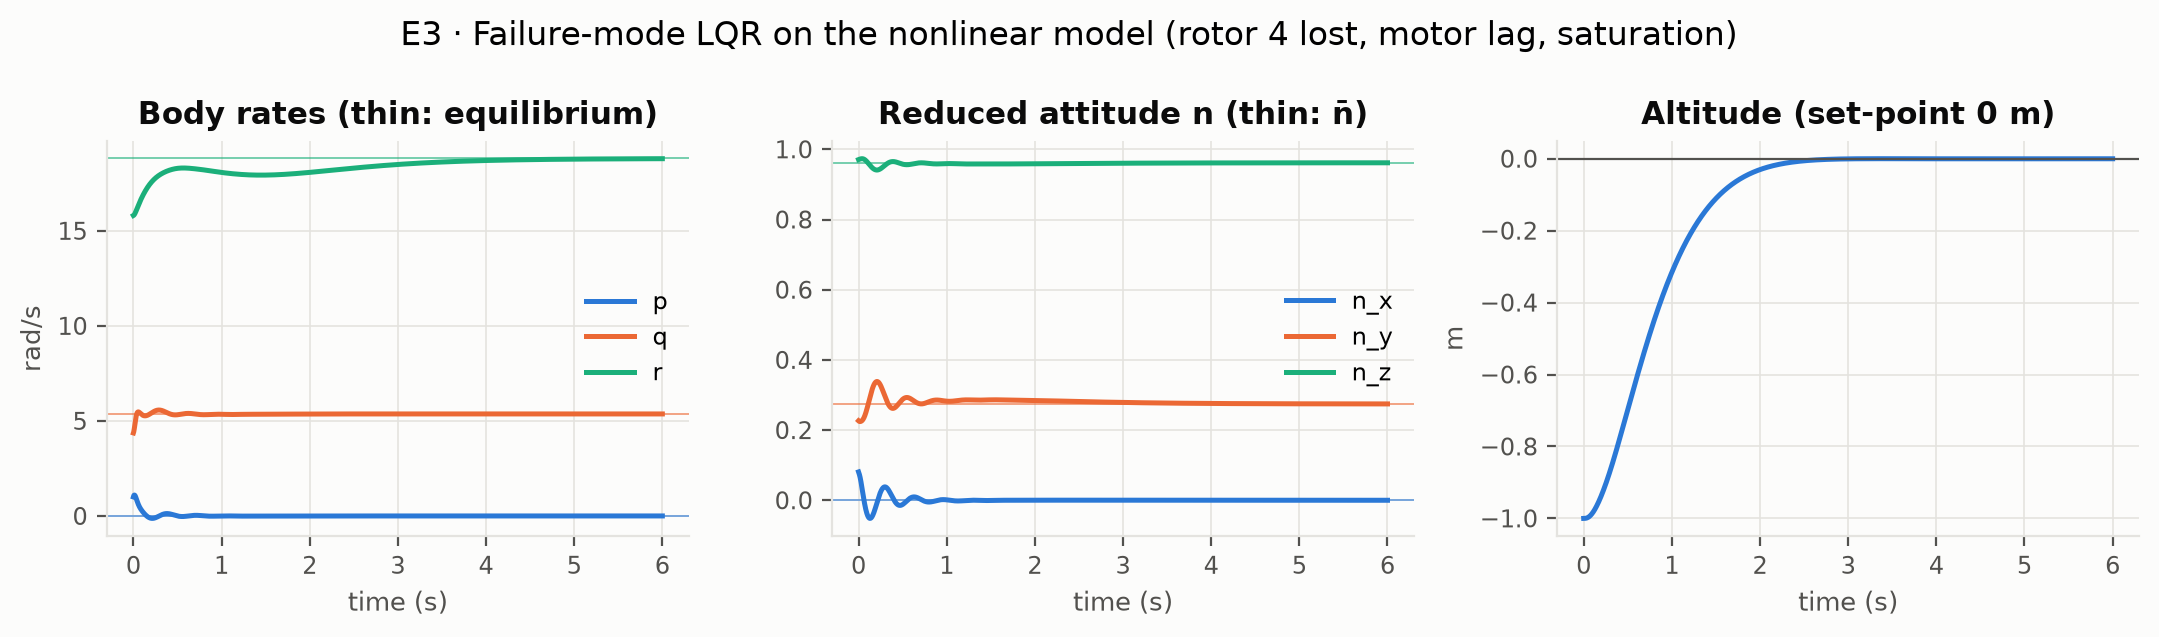
\includegraphics[width=\linewidth]{figures/e3_failed_lqr_nonlinear.png}
\caption{Failure LQR on the nonlinear model (rotor 4 lost, motor lag, thrust limits), starting from a perturbed relaxed hover 1\,m below the set-point. Thin lines: equilibrium values.}\label{fig:lqr}
\end{figure}
\begin{figure}[h]
\centering
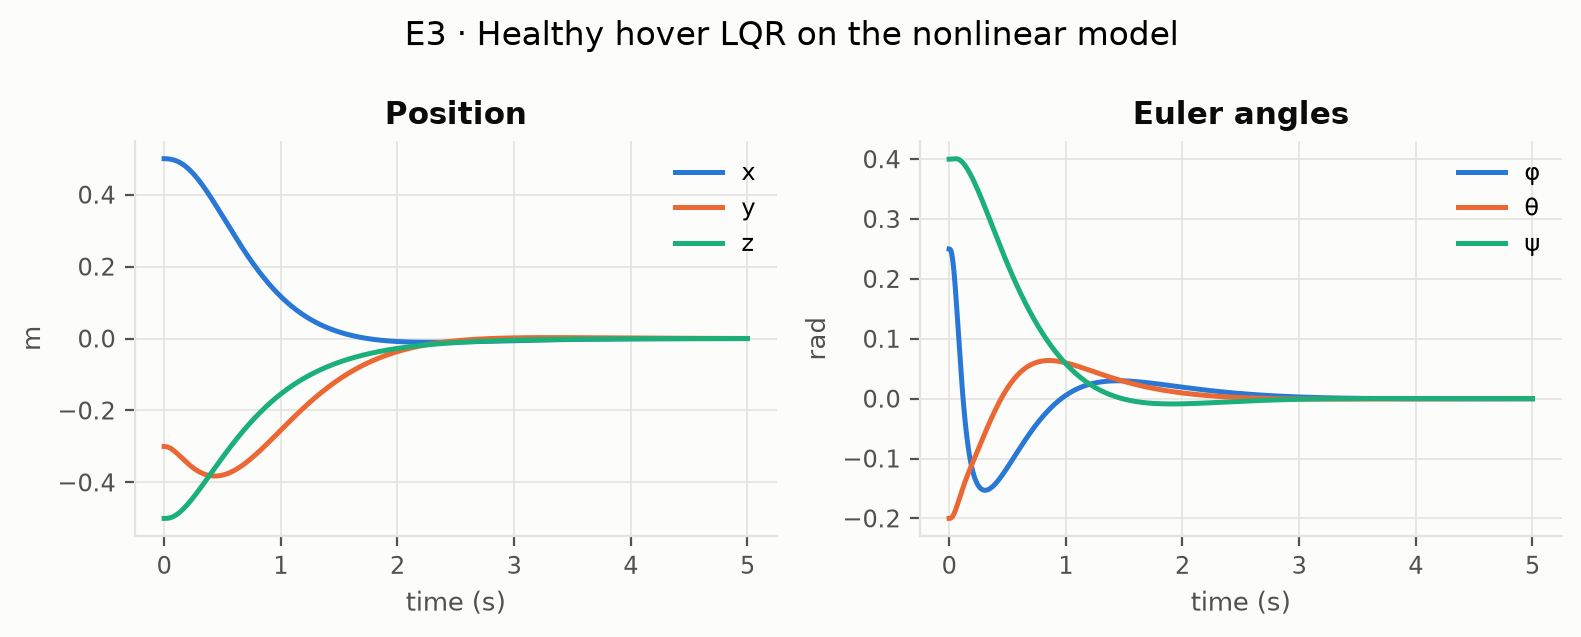
\includegraphics[width=0.75\linewidth]{figures/e3_healthy_lqr_nonlinear.png}
\caption{Healthy LQR on the nonlinear model from an offset, tilted start.}\label{fig:lqr-healthy}
\end{figure}

%=====================================================================
\section{Learning the model error: residual Koopman models (RQ1)}\label{sec:koopman}
%=====================================================================
This section answers the prediction half of RQ1: which model best predicts how the failed drone will move? We compare three predictors trained and tested on exactly the same data (experiment E6).

\subsection{Hypotheses}
Before running the experiment we wrote down what we expected (from the proposal):
\begin{description}[leftmargin=1.2em]
  \item[H1.] A Koopman model of the full dynamics, learned from failed-drone data, has eigenvalues outside the unit circle and loses to a trivial ``nothing changes'' predictor at long horizons. (Our proposal found this for a healthy drone.)
  \item[H2.] The residual model has a lower multi-step prediction error than both the physics model and the full Koopman model.
  \item[H4.] The residual model reaches a given error with less data than the full Koopman model. (H3 concerns MPC and is tested in Section~\ref{sec:mpc}.)
\end{description}

\subsection{Data}
\paragraph{Why a separate truth plant.} The data come from truth plant A (Section~\ref{sec:truth}), not from the nominal model. Otherwise the physics model would already be perfect and there would be nothing to learn.

\paragraph{How episodes are generated.} Each episode lasts 4\,s with rotor 4 failed:
\begin{enumerate}
  \item The drone starts near the relaxed hover, with random deviations drawn uniformly: body rates $\pm2$\,rad/s, tilt $\pm0.15$ in $n_x$ and $n_y$, height and vertical speed $\pm0.5$.
  \item It is flown by the failure LQR designed on the \emph{nominal} parameters. A learned model needs to see the drone respond to many different inputs, so we add a random \emph{excitation}: every 50\,ms a new random offset, uniform in $\pm0.35$\,N, is added to each of the three thrust commands (then clipped to the limits).
  \item The simulator runs at 1\,ms; the controller and the recorded data run at $\Ts = 5$\,ms.
  \item At every sample we record the measured state as a deviation from the relaxed hover, $\vect x = (p,q,r,n_x,n_y,z,v_z) - \bar{\vect s}$; the command deviation $\vect u = (f_1,f_2,f_3) - \bar{\vect f}$; and $\hat{\vect f}$, the nominal first-order filter of the commands. The true motor thrust is not used, because a real flight computer does not measure it.
  \item Episodes in which the tilt deviation exceeds 0.6 (the drone has left the region of interest) are discarded.
\end{enumerate}
Training uses 40 episodes (32,000 samples, seed 11). Testing uses 10 new episodes from plant A (seed 12) and 10 from the held-out plant B (seed 13). A second training set of 40 episodes, each from a randomly drawn plant (seed 21), tests whether varied training data helps.

\subsection{The three predictors}
\paragraph{1. Analytical (physics only).} The 10-state linear model of Section~\ref{sec:linmodels} (7 states and 3 motor states, nominal parameters), discretized exactly with a zero-order hold at 5\,ms:
\begin{equation}
  \vect s_{k+1} = A_d\vect s_k + B_d\vect u_k, \qquad \vect s = (\vect x, \hat{\vect f}) \in\mathbb R^{10}.
\end{equation}
It uses no data at all.

\paragraph{2. Full-state EDMDc.} Everything is learned from data~\cite{williams2015edmd,korda2018linear}. We take the 9-number vector $\vect\xi = (p,q,r,n_x,n_y,v_z,\hat f_1,\hat f_2,\hat f_3)$; height $z$ is left out because it is just the integral of $v_z$. Each entry is \emph{standardized} (the training mean subtracted and the result divided by the training standard deviation), giving $\tilde{\vect\xi}$. The dictionary is
\begin{equation}
  \psi(\vect\xi) = \big(\;1,\;\; \tilde\xi_1,\dots,\tilde\xi_9,\;\; \tilde\xi_1^2,\, \tilde\xi_1\tilde\xi_2,\,\dots,\,\tilde\xi_9^2\;\big),
\end{equation}
that is, a constant, the 9 standardized values and all 45 products of two of them: $1 + 9 + 45 = 55$ functions. We then fit the lifted linear model
\begin{equation}
  \psi(\vect\xi_{k+1}) \approx A\,\psi(\vect\xi_k) + B\,\vect u_k
\end{equation}
by ridge regression over all training pairs (regularization $\lambda = 10^{-6}$). To predict, we lift the starting state once, iterate $\vect\zeta\leftarrow A\vect\zeta + B\vect u$ (we write $\vect\zeta$ for the lifted state here, to avoid confusion with the height $z$), read $\vect\xi$ back from the 9 linear coordinates of $\vect\zeta$, and integrate $v_z$ with the trapezoid rule to get the height $z$.

\paragraph{3. Residual EDMDc (proposed).} Keep the physics model and learn only its one-step error. For every training pair we compute what the physics model would have predicted and the difference to what really happened:
\begin{equation}
  \vect e_{k+1} = \vect x_{k+1} - \big[A_d\vect s_k + B_d\vect u_k\big]_{1:7}.
\end{equation}
We regress $\vect e_{k+1}$ on the same kind of quadratic dictionary, now built from $(\vect\xi_k, \vect u_k)$ (the same 9 values plus the 3 commands, standardized; $1 + 12 + 78 = 91$ functions), with ridge regularization $\lambda = 10^{-3}$, giving a matrix $W$. The prediction is
\begin{equation}
  \vect x_{k+1} = \big[A_d\vect s_k + B_d\vect u_k\big]_{1:7} + \operatorname{clip}\big(W^\top\psi(\vect\xi_k,\vect u_k),\; \pm\vect d_{\max}\big),
\end{equation}
where $\vect d_{\max}$ is the 99.5th percentile of the absolute training residuals, per state. The clipping, borrowed from Todde et al.~\cite{todde2026residual}, prevents the learned part from producing a correction larger than anything seen in training, for example when the drone is far from the training data.

\paragraph{Why we call it a residual Koopman model.} Strictly, this model uses the EDMD dictionary and least squares to learn a \emph{one-step} correction; unlike the full-state EDMDc model it does not propagate a lifted linear state, and the input enters it nonlinearly (through products such as $\xi_i u_j$). It is closer to a polynomial regression of the error than to a linear Koopman predictor, and we keep the name only because it follows the same construction as the residual models in the literature~\cite{todde2026residual,narayanan2026rkmpc}. What keeps the MPC problem convex is not linearity of this model but the way it is used: it is evaluated outside the optimization (Section~\ref{sec:mpc}).

\begin{plain}
The physics model provides most of the prediction: it already knows that the drone spins, how fast, and how it responds to each rotor. The learned part only has to describe a small correction, such as ``the drone sinks a little faster than the physics says when it spins fast'', and that correction is much easier to learn than the whole motion.
\end{plain}

\begin{codebox}{fitting the residual}
\begin{lstlisting}
for X, fe, U in zip(data.x, data.fe, data.u):          # every training episode
    for k in range(len(U)):
        x1n, _ = nom.step(X[k], fe[k], U[k])            # physics prediction
        E.append(X[k + 1] - x1n)                        # what it got wrong
        F.append(np.concatenate((X[k, XI_IDX], fe[k], U[k])))
dic = Dictionary(F.mean(0), F.std(0) + 1e-9)           # standardize, quadratic features
W = ridge(dic(F), E, lam)                               # (Phi'Phi + lam I)^-1 Phi'E
d_max = np.percentile(np.abs(E), 99.5, axis=0)          # clipping level
\end{lstlisting}
\end{codebox}

\paragraph{4. No-change baseline.} The prediction is simply the starting state, held forever. Any model worse than this is useless at that horizon.

\subsection{How prediction error is measured}
From each test episode (800 samples) we start a prediction every 40 samples (0.2\,s), as long as the longest horizon (600 samples) still fits: 5 starts per episode, all in the first 0.8\,s, so 50 starts per test set. Each predictor is given the true starting state and the recorded inputs, and it predicts \emph{open loop}, that is, without seeing any later measurement. We compare the prediction with the true trajectory at horizons from 5\,ms to 3\,s. Each state's error is divided by that state's standard deviation in the training data (so rad/s and metres can be combined), squared, averaged over all start times and all 7 states, and square-rooted:
\begin{equation}
  \text{NRMSE}(h) = \sqrt{\frac{1}{7N_{\text{starts}}}\sum_{\text{starts}}\sum_{i=1}^{7}\left(\frac{\hat x_i(h) - x_i(h)}{\operatorname{std}_i}\right)^2 }.
\end{equation}
(To keep a diverging model from producing overflow, each squared error is capped at $10^{12}$ before averaging.) A value of 1 means the error is as large as the typical variation of the states; the no-change baseline sits at about 2.4.

\subsection{Results}
\begin{table}[h]
\centering\small
\caption{Normalized multi-step prediction error (lower is better), models trained on family A.}\label{tab:pred}
\begin{tabular}{lccccccc}
\toprule
& \multicolumn{4}{c}{Test family A} & \multicolumn{3}{c}{Test family B (held out)} \\
\cmidrule(lr){2-5}\cmidrule(lr){6-8}
Predictor & 20\,ms & 0.1\,s & 1\,s & 2\,s & 0.1\,s & 1\,s & 2\,s \\
\midrule
Analytical & 0.65 & 3.17 & 7.09 & 7.93 & 4.31 & 7.94 & 6.95 \\
Full-state EDMDc & \textbf{0.04} & 0.17 & 0.91 & 3.45 & 6.09 & 26.2 & 131 \\
Residual EDMDc & 0.10 & \textbf{0.15} & \textbf{0.64} & 2.71 & 5.98 & 19.9 & 24.0 \\
No change & 0.81 & 2.42 & 2.38 & 2.51 & 2.51 & 2.44 & 2.41 \\
\bottomrule
\end{tabular}
\end{table}

\begin{figure}[h]
\centering
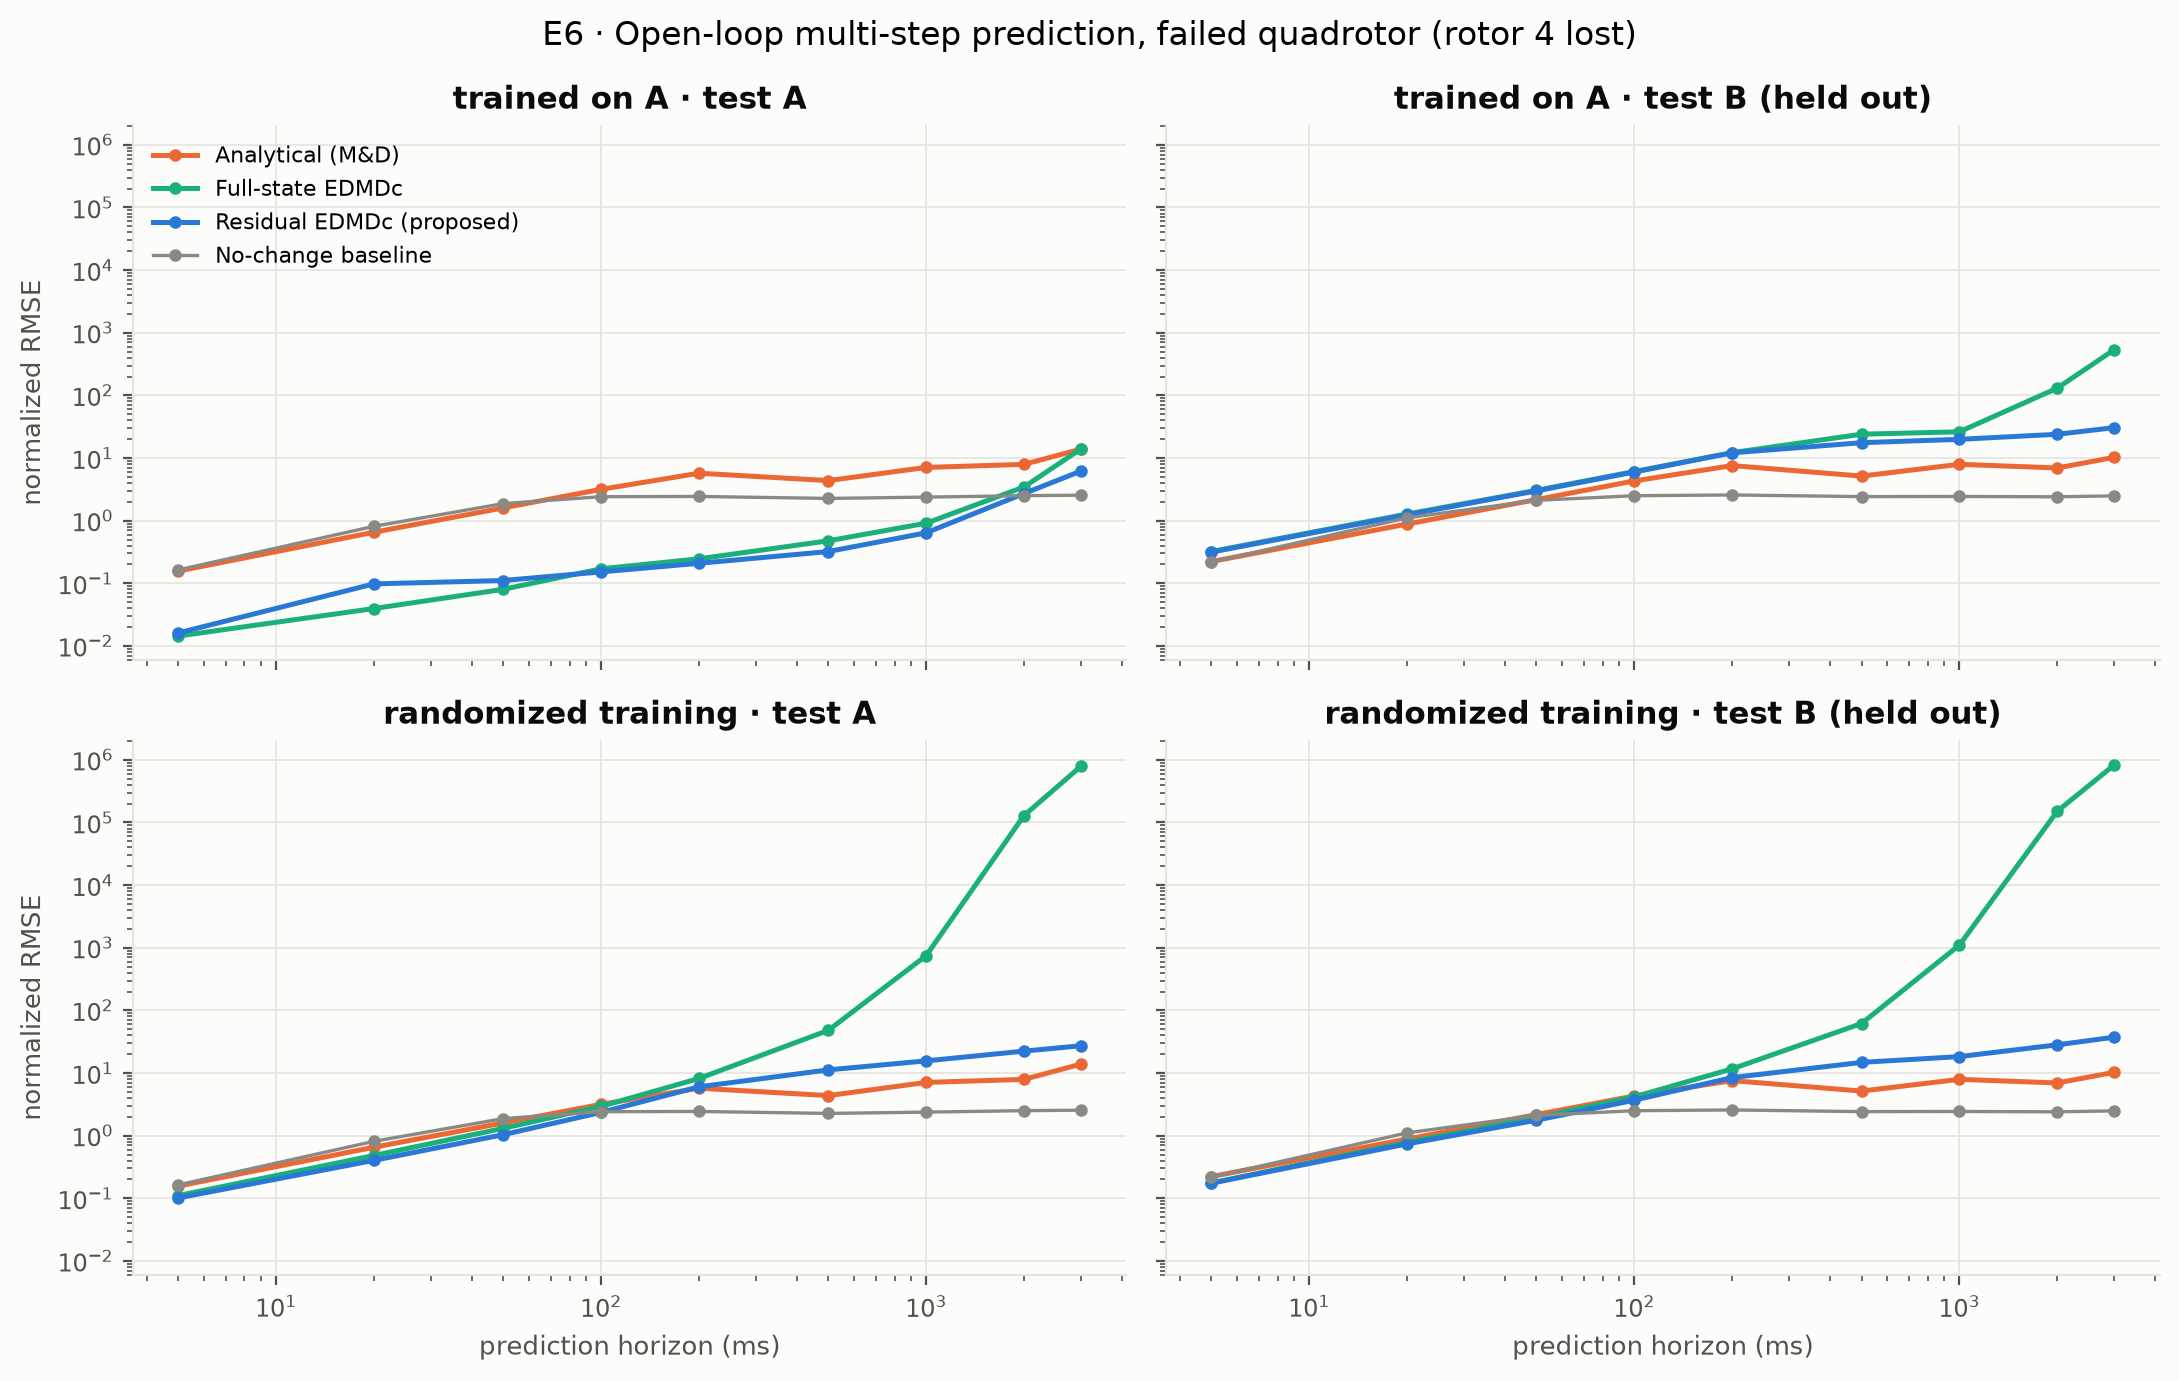
\includegraphics[width=0.95\linewidth]{figures/e6_multistep_error.png}
\caption{Multi-step prediction error against horizon (both axes logarithmic). Top: trained on family A. Bottom: trained on randomized plants. Left: tested on family A; right: tested on the held-out family B.}\label{fig:pred}
\end{figure}

\paragraph{H2 (residual is best): supported on the training plant.} On new episodes from plant A, the residual model is the most accurate of the three models at every horizon from 100\,ms on, and the most accurate predictor overall from 100\,ms to 1\,s (Table~\ref{tab:pred}, Figure~\ref{fig:pred} top left). At 1\,s its error is 0.64, against 0.91 for full-state EDMDc and 7.09 for the physics model. At short horizons (5 to 50\,ms) the full-state model is better, by a factor of 2.5 at 20\,ms (0.04 against 0.10). The physics model is worse than the no-change baseline from about 100\,ms on: its undamped modes and the unmodelled thrust loss make it drift away. At 2\,s even the residual model is behind the no-change baseline, so long open-loop horizons need feedback, which is what MPC provides by re-planning every 5\,ms.

\paragraph{H1 (full model is unstable): supported.} The learned $55\times55$ matrix $A$ of the full-state model has 4 eigenvalues outside the unit circle (spectral radius 1.0070, Figure~\ref{fig:eigs}). The true open-loop model has undamped modes that lie exactly on the unit circle in discrete time, so this is a small outward push of modes that are only marginally stable in reality, not a qualitatively different defect. Over many steps, however, it makes errors grow, and the model falls behind the no-change baseline by 2\,s and explodes at 3\,s (error 14.1). This repeats, in the failed regime, what our proposal found for a healthy drone (with full-state EDMDc, 10 of 22 eigenvalues were outside the unit circle).

\begin{figure}[h]
\centering
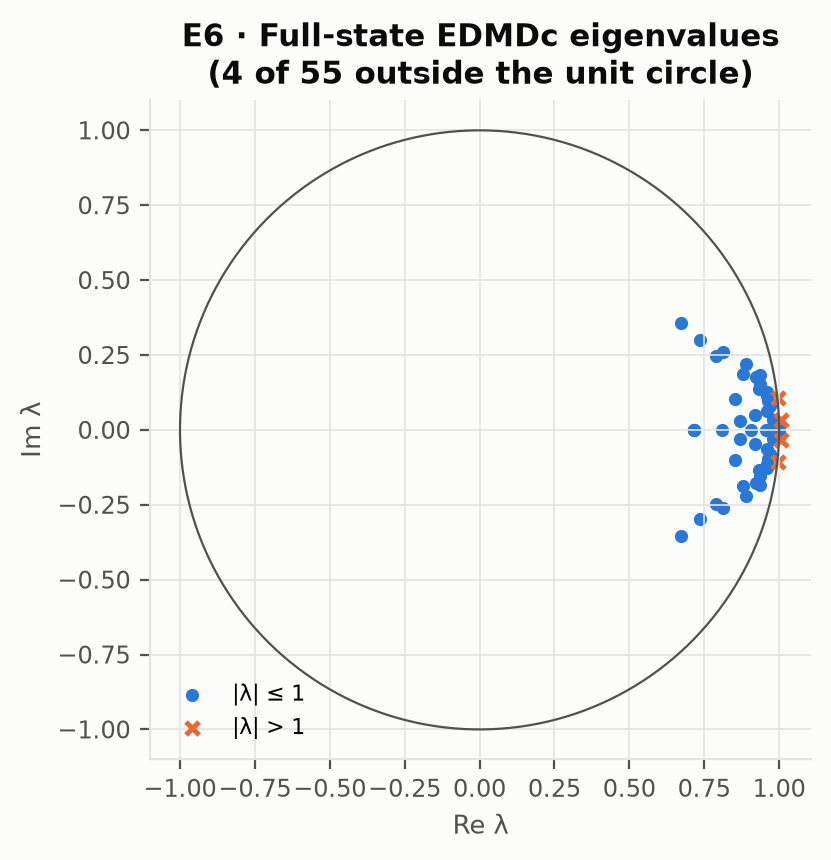
\includegraphics[width=0.45\linewidth]{figures/e6_full_edmdc_eigs.png}
\caption{Eigenvalues of the learned full-state EDMDc matrix. Crosses lie outside the unit circle, so their modes grow.}\label{fig:eigs}
\end{figure}

\paragraph{H4 (less data): supported, with one exception.} Figure~\ref{fig:eff} repeats the training with 2, 5, 10, 20 and 40 episodes and measures the error at a 0.5\,s horizon. The residual model trained on only 10 episodes (error 0.42) is already better than the full-state model trained on all 40 (0.48). This matters because data from failed flights is scarce: such flights often end in a crash. The same advantage of residual models has been reported for soft robots, ground vehicles and quadrupeds~\cite{bruder2025residual,fu2025residual,narayanan2026rkmpc}; we confirm it in the spinning regime. The curves are not monotone: at 5 episodes the full-state model is slightly better (0.93 against 1.02).

\begin{figure}[h]
\centering
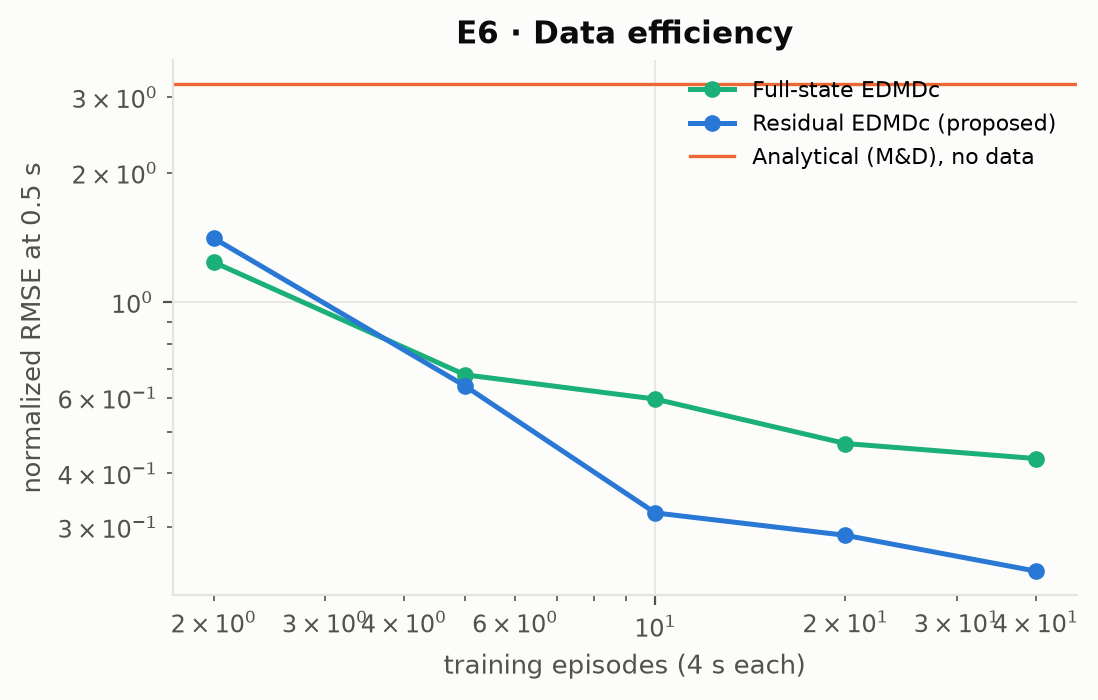
\includegraphics[width=0.55\linewidth]{figures/e6_data_efficiency.png}
\caption{Prediction error at 0.5\,s against the number of training episodes (family A). The flat line is the physics model, which uses no data.}\label{fig:eff}
\end{figure}

\paragraph{Generalization: not achieved.} On the held-out plant B, both models trained on plant A are \emph{worse} than the physics model (Table~\ref{tab:pred}, right). The learned correction is specific to the plant it saw: it ``corrects'' B as if it were A, which makes things worse. Training on randomized plants, one random plant per episode, does not solve this. It helps the residual model on B only up to about 100\,ms (error 3.68 against 4.31 for the physics model) and makes both learned models worse on A (the full-state model trained this way even diverges, spectral radius 1.028). The likely reason is that a single state sample does not reveal which plant the drone is: the motor time constant and the thrust loss show only in how the state changes over several steps. A static regression then learns an average correction that fits no plant well. This points to online adaptation: because the residual is linear in $W$, it can be updated during flight by recursive least squares. Online-adapted Koopman models exist for healthy quadrotors~\cite{jin2025dekc} and for loss-of-effectiveness faults~\cite{lee2024koopmanftmpc}.

\subsection{What this means for RQ1}
\begin{plain}
On the drone it was trained on, learning only the error of the physics model gives the best predictions from 0.1 to 1\,s, and with 10 training episodes it is more accurate than learning everything from 40 episodes. But the learned correction does not carry over to a drone with different parameters. In its current form it is a calibration for one vehicle, not a general model of rotor failure.
\end{plain}

%=====================================================================
\section{Model predictive control with the learned residual (RQ1)}\label{sec:mpc}
%=====================================================================
This section answers the control half of RQ1 and tests hypothesis \textbf{H3}: a residual Koopman MPC removes the steady error that model mismatch causes in a controller designed on the physics model (experiment E7).

\subsection{The MPC problem}
At every sample (5\,ms) the controller measures the current state, builds $\vect s_0 = (\vect x, \hat{\vect f})$ and solves
\begin{equation}\label{eq:mpc}
\begin{aligned}
\min_{\vect u_0,\dots,\vect u_{N-1}} \;& \textstyle\sum_{j=0}^{N-1}\big(\vect s_j^\top Q\,\vect s_j + \vect u_j^\top R\,\vect u_j\big) + \vect s_N^\top P_N\,\vect s_N\\
\text{subject to }\;& \vect s_{j+1} = A_d\vect s_j + B_d\vect u_j + \hat{\vect d},\qquad j = 0,\dots,N-1,\\
& f_{\min}-\bar f_i \;\le\; u_{j,i} \;\le\; f_{\max}-\bar f_i .
\end{aligned}
\end{equation}
\begin{itemize}
  \item The prediction model is the 10-state analytical model of Section~\ref{sec:koopman}.
  \item The horizon is $N = 20$ steps of 5\,ms, so the controller looks 100\,ms ahead.
  \item $Q$ and $R$ are the same weights as the failure LQR, so the two controllers aim for the same thing.
  \item The \emph{terminal cost} $P_N$ is the solution of the discrete-time Riccati equation for $(A_d, B_d, Q, R)$. It stands in for the cost after the horizon; with it, the MPC behaves like the discrete LQR whenever the limits are not active, which our tests check.
  \item The input limits are the motor thrust limits, written as deviations from the trim.
\end{itemize}
Only the first input $\vect u_0$ is applied; at the next sample the problem is solved again from the new measurement.

\subsection{Where the learned residual enters}
The \textbf{analytical MPC} uses $\hat{\vect d} = 0$. The \textbf{residual Koopman MPC} evaluates the learned residual once per sample, at the current state and previous input, \emph{outside} the optimization, and adds it to every predicted step as a known constant $\hat{\vect d}$ (a ``measured disturbance''), as Todde et al. do~\cite{todde2026residual}. The learned part is therefore not a decision variable, the constraints stay linear, and~\eqref{eq:mpc} stays a convex QP that solves reliably every time. The price is that the optimizer does not know how the residual would change with its own choice of inputs or along the predicted trajectory: the correction is frozen at its current value for the whole 100\,ms horizon.

\begin{plain}
The physics model plans the next 100\,ms; the learned residual tells it ``at the moment the real drone drifts this much more per step than you think'', and the plan compensates for that drift.
\end{plain}

\begin{codebox}{building and solving the QP once per sample}
\begin{lstlisting}
# built once: CVXPY parameters x0 and d, variables X (states) and U (inputs)
for j in range(N):
    cons += [X[:, j + 1] == Ad @ X[:, j] + Bd @ U[:, j] + self.d,
             U[:, j] >= lo, U[:, j] <= hi]
    cost += cp.quad_form(X[:, j], Q) + cp.quad_form(U[:, j], R)
cost += cp.quad_form(X[:, N], PN)                       # DARE terminal cost

# every sample
d[:7] = self.residual.residual(x7, self.fe, self.u_prev) # learned part, outside the QP
self.x0.value, self.d.value = np.concatenate((x7, self.fe)), d
self.prob.solve(solver=cp.OSQP, warm_start=True, eps_abs=1e-5, eps_rel=1e-5)
u = self.U.value[:, 0]                                   # apply the first move only
\end{lstlisting}
\end{codebox}
The problem is modelled with CVXPY~\cite{diamond2016cvxpy} and solved with OSQP~\cite{stellato2020osqp}, an operator-splitting QP solver; ``warm start'' reuses the previous solution as the starting guess.

\subsection{Experiment: steady altitude error under mismatch}
All three controllers (LQR, analytical MPC, residual Koopman MPC) are designed on the nominal parameters and flown on the mismatched truth plants. The residual is the one trained on family A in Section~\ref{sec:koopman}. Each run starts 1\,m below the set-point near the relaxed hover and lasts 8\,s; the steady error is the mean height over the last 2\,s. We use one run per plant and controller, because the steady state does not depend on the starting point. To see which effect causes the error, we also test each family without its thrust loss, and the nominal plant with only that family's thrust loss.

\begin{table}[h]
\centering\small
\caption{Steady altitude error near the relaxed hover (set-point 0\,m). The last column compares the \emph{magnitude} of the residual-MPC error with the LQR error; for plant B (full) the sign also changes.}\label{tab:mpc}
\begin{tabular}{lcccc}
\toprule
Plant & LQR & MPC, analytical & MPC, residual & Change \\
\midrule
A (full) & $-0.285$\,m & $-0.286$\,m & $\mathbf{-0.193}$\,m & $-32$\% \\
A without thrust loss & $-0.154$\,m & $-0.154$\,m & $-0.066$\,m & $-57$\% \\
Nominal + A's thrust loss only & $-0.100$\,m & $-0.101$\,m & $-0.033$\,m & $-67$\% \\
B (full, held out) & $-0.029$\,m & $-0.033$\,m & $+0.022$\,m & $-25$\% \\
B without thrust loss & $+0.112$\,m & $+0.111$\,m & $+0.164$\,m & $+47$\% \\
Nominal + B's thrust loss only & $-0.174$\,m & $-0.177$\,m & $-0.107$\,m & $-39$\% \\
\bottomrule
\end{tabular}
\end{table}

\begin{figure}[h]
\centering
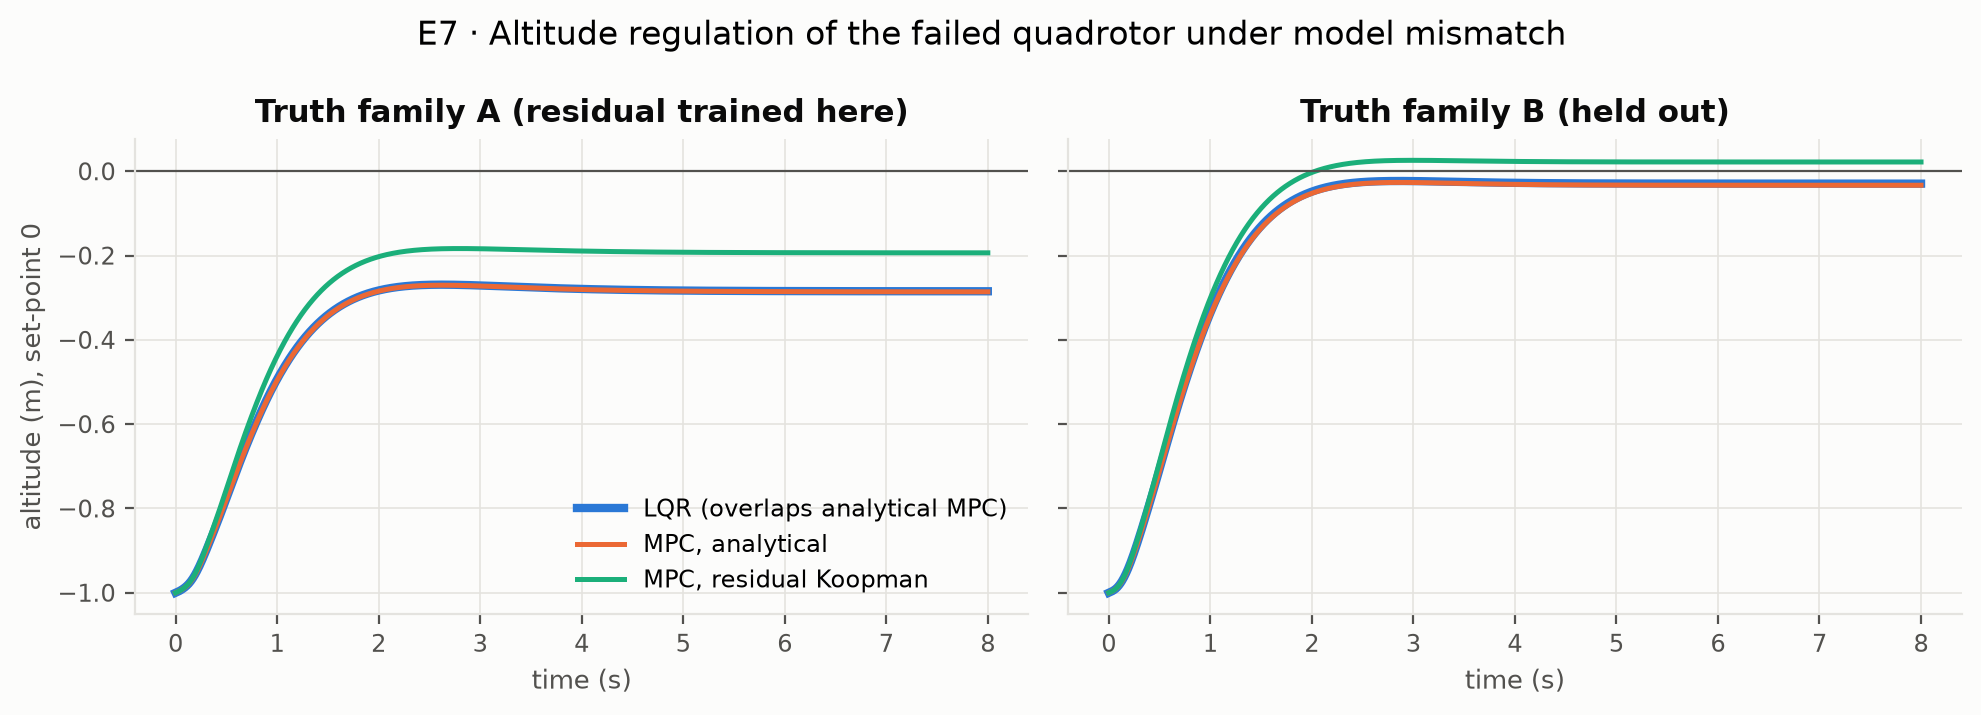
\includegraphics[width=\linewidth]{figures/e7_altitude.png}
\caption{Height of the failed drone under model mismatch for the three controllers (LQR and analytical MPC overlap). Left: family A, on which the residual was trained. Right: held-out family B.}\label{fig:mpc}
\end{figure}

\paragraph{Results.} On plant A, LQR and the analytical MPC both settle 0.29\,m too low; they are practically identical, because near the equilibrium the thrust limits are not reached and the MPC then acts like the LQR. The thrust loss alone causes 0.10\,m and the inertia and motor mismatch alone 0.15\,m; the effects are not exactly additive (together 0.29\,m). The residual Koopman MPC settles 0.19\,m low, a 32\% smaller error, and it reduces the error for each separate effect of plant A. On the held-out plant B the effects partly cancel. The residual MPC still reduces the error for the full plant and for its thrust loss alone, but when B's thrust loss is removed it makes the error 47\% \emph{larger}: the correction learned on A pushes in the wrong direction for that plant. This is the generalization problem of Section~\ref{sec:koopman} again. H3 is therefore only partly supported: on the training plant the error is reduced by 32\%, not removed, and on a held-out variant it grows. The errors on plant B are only a few centimetres, so their percentages should not be over-read.

The residual reduces the error but does not remove it. The classical way to remove a steady error caused by a constant mismatch is integral action, or an ``offset-free'' MPC that estimates a constant disturbance from the measurements; in theory it removes such an error completely. This is the most important missing baseline: until it is compared, the 32\% reduction shows that the residual carries useful information, not that it is the best way to remove the bias. A residual could still help where integral action is slow, for example during transients.

\paragraph{Computation time.} The QP solver needs a median of 0.73\,ms per sample. Through the CVXPY modelling layer the median wall-clock time is 4.4\,ms, which leaves almost no margin to the 5\,ms sample period. A real-time version would call the solver directly.

%=====================================================================
\section{How long may fault detection take? (RQ2, empirical)}\label{sec:delay}
%=====================================================================
\subsection{The failure timeline}
Figure~\ref{fig:timeline} shows what happens around a failure. At $t=0$ rotor 4 stops. The flight computer does not know this yet, so the healthy controller keeps flying. At $t=\tau$ (the \emph{detection delay}) a detector raises the alarm and a supervisor switches to the failure-mode strategy, which must \emph{capture} the drone into the relaxed hover from wherever it has drifted.

\begin{figure}[h]
\centering
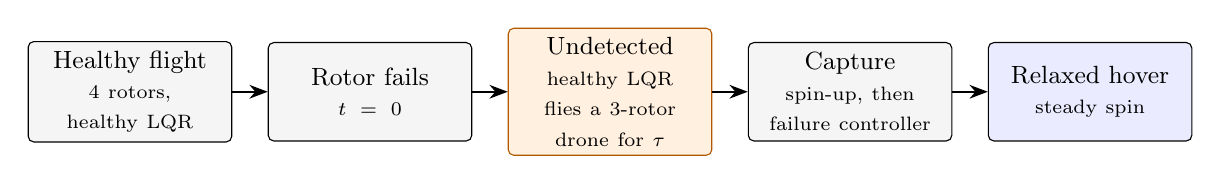
\begin{tikzpicture}[>=Stealth, box/.style={draw, rounded corners=2pt, align=center, minimum height=1.25cm, text width=2.35cm, font=\small}]
  \node[box, fill=gray!8] (a) {Healthy flight\\ \scriptsize 4 rotors, healthy LQR};
  \node[box, fill=gray!8, right=0.45cm of a] (b) {Rotor fails\\ \scriptsize $t = 0$};
  \node[box, fill=orange!12, draw=orange!70!black, right=0.45cm of b] (c) {Undetected\\ \scriptsize healthy LQR flies a 3-rotor drone for $\tau$};
  \node[box, fill=gray!8, right=0.45cm of c] (d) {Capture\\ \scriptsize spin-up, then failure controller};
  \node[box, fill=blue!8, right=0.45cm of d] (e) {Relaxed hover\\ \scriptsize steady spin};
  \foreach \u/\v in {a/b,b/c,c/d,d/e} \draw[->,thick] (\u) -- (\v);
\end{tikzpicture}
\caption{The failure timeline. RQ2 is about the orange phase: how long it may last.}\label{fig:timeline}
\end{figure}

\subsection{Why the undetected phase is dangerous: a simple bound}
Right after the failure the drone is still near level hover, so the body rates are small and the gyroscopic terms in~\eqref{eq:rot} are negligible. The roll equation then reduces to
\begin{equation}
  I^B_{xx}\,\dot p = l\,(f_2 - f_4) = l\,f_2,
\end{equation}
because $f_4 = 0$. Rotor 2, opposite the failed rotor, now pushes one side up with nothing to balance it. The healthy controller notices the roll and reduces $f_2$, but it keeps its motors running, and a running motor cannot go below its idle thrust $f_{\min}$. Hence
\begin{equation}
  \dot p \;\ge\; \frac{l\,f_{\min}}{I^B_{xx}} = \frac{0.17\times0.2}{3.2\times10^{-3}} = 10.6\ \text{rad/s}^2 .
\end{equation}
This holds for \emph{any} healthy controller whose motor allocation keeps running motors at or above idle, as standard autopilots do, however it is tuned. Integrating twice gives a lower bound on the roll angle, $\tfrac12(lf_{\min}/I^B_{xx})t^2$.

Figure~\ref{fig:undetected} shows the simulation for three tunings of the healthy LQR ($\alpha = 0.3$, 1 and 3): the tilt reaches about 12 to 15$^\circ$ at 100\,ms and 33 to 43$^\circ$ at 200\,ms, so a more aggressive tuning helps only a little. Rotor 2's thrust falls close to its idle limit within about 100\,ms; the controller then has no roll authority left.

\begin{figure}[h]
\centering
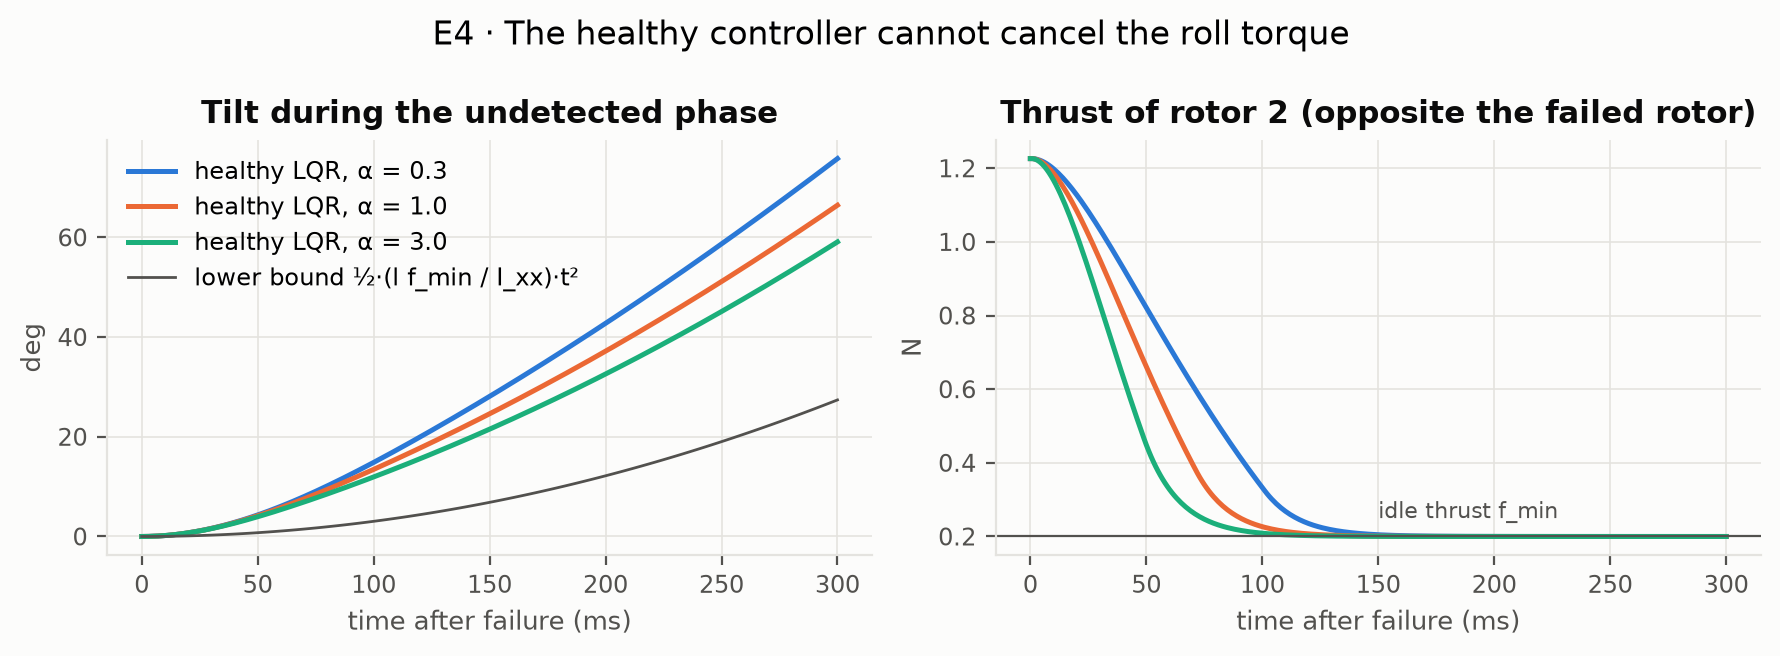
\includegraphics[width=\linewidth]{figures/e4_undetected_phase.png}
\caption{Undetected phase. Left: tilt for three healthy-controller tunings with the analytic lower bound. Right: thrust of rotor 2, which drops to idle.}\label{fig:undetected}
\end{figure}

\subsection{Experimental design (E4)}
\paragraph{Scenario.} The drone hovers at height 0 on the nominal plant. At $t=0$ rotor 4 fails. Until $t=\tau$ the healthy LQR flies (its command to rotor 4 has no effect). At $t=\tau$ a supervisor switches to one of these failure strategies:
\begin{itemize}
  \item \textbf{Direct LQR}: the failure LQR is switched on at once.
  \item \textbf{Spin-up, then LQR} (the strategy of~\cite{mueller2014stability}, used in their flight; the details below are read from their Fig.~4): rotors 1 and 3 run at a fixed thrust $f_{\text{spin}}$, rotor 2 is stopped, with no attitude feedback, until the rotation rate exceeds 10\,rad/s; then the failure LQR takes over. We use $f_{\text{spin}} = 2.95$\,N (read from the flight data) and, as a sensitivity case, $mg/2 = 2.45$\,N.
\end{itemize}
At the switch, the failure controller's motor-thrust estimate is initialized from the supervisor's filter of the commands it sent before, never from the true thrust. Each run lasts 10\,s, with the controller at 1\,ms.

\begin{codebox}{the detection-delay supervisor}
\begin{lstlisting}
def alive(self, t):                     # which rotors produce thrust
    return np.array([True, True, True, t < self.t_fail])

def __call__(self, t, x):
    if t < self.t_fail + self.tau:      # failure not yet detected
        u = self.healthy(t, x)          # (also updates a filter of the commands sent)
        return u
    if not self.switched:               # first call after detection
        self.failure.reset(self.f_cmd_est)
        self.switched = True
    return self.failure(t, x)           # spin-up, then failure LQR
\end{lstlisting}
\end{codebox}

\paragraph{Success criterion, fixed before the runs.} It is written in \texttt{metrics.py} and was not changed after seeing results. A run is
\begin{itemize}
  \item \textbf{captured} if, over the last 1\,s of a run that did not stop early, the reduced attitude is within 0.05 of $\bar{\vect n}$ and the body rates are within 2\,rad/s of $\bar{\vect\omega}$;
  \item \textbf{safe} if it is captured, \emph{and} the height loss (starting height minus lowest height) is below 2\,m, \emph{and} the drone never turns upside down ($n_z > 0$ throughout).
\end{itemize}

\paragraph{Monte Carlo.} A real failure does not happen at a perfect hover. For each delay $\tau = 0, 5, 10, \dots, 60$\,ms and each spin-up thrust we ran 40 simulations from random pre-failure states (velocity with standard deviation 0.3\,m/s, Euler angles 3$^\circ$, body rates 0.3\,rad/s; the same 40 seeds for every delay). The estimated probability of a safe recovery is $\hat p = k/n$ ($k$ safe runs out of $n=40$). Its 95\% \emph{Wilson} confidence interval is
\begin{equation}
  c \pm h, \qquad c = \frac{\hat p + z^2/(2n)}{1+z^2/n}, \qquad h = \frac{z}{1+z^2/n}\sqrt{\frac{\hat p(1-\hat p)}{n} + \frac{z^2}{4n^2}}, \qquad z = 1.96 .
\end{equation}
Unlike the textbook interval $\hat p \pm z\sqrt{\hat p(1-\hat p)/n}$, it does not collapse to zero width when $\hat p$ is 0 or 1. We summarize each curve by $\tau_{90}$ and $\tau_{50}$, the delays at which $\hat p$ first falls below 0.9 and 0.5 (linear interpolation between grid points). We also swept $\tau$ from 0 to 300\,ms in 10\,ms steps from the exact hover, for all three strategies, and for three healthy-controller tunings with the 2.95\,N spin-up.

\subsection{Results}
\begin{table}[h]
\centering\footnotesize
\caption{Spin-up then LQR: fraction of safe recoveries in 40 random starts per delay, with 95\% Wilson intervals.}\label{tab:delay}
\setlength{\tabcolsep}{3pt}
\begin{tabular}{lccccccc}
\toprule
Delay $\tau$ & 0\,ms & 5\,ms & 10\,ms & 15\,ms & 20\,ms & 30\,ms & 40\,ms \\
\midrule
2.95\,N & 1.00 & 1.00 & 0.97 & 0.80 & 0.42 & 0.17 & 0.07 \\
 & [0.91, 1] & [0.91, 1] & [0.87, 1] & [0.65, 0.90] & [0.29, 0.58] & [0.09, 0.32] & [0.03, 0.20] \\
\midrule
2.45\,N & 1.00 & 0.95 & 0.82 & 0.45 & 0.28 & 0.07 & 0.07 \\
 & [0.91, 1] & [0.83, 0.99] & [0.68, 0.91] & [0.31, 0.60] & [0.16, 0.43] & [0.03, 0.20] & [0.03, 0.20] \\
\bottomrule
\end{tabular}
\end{table}

\begin{figure}[h]
\centering
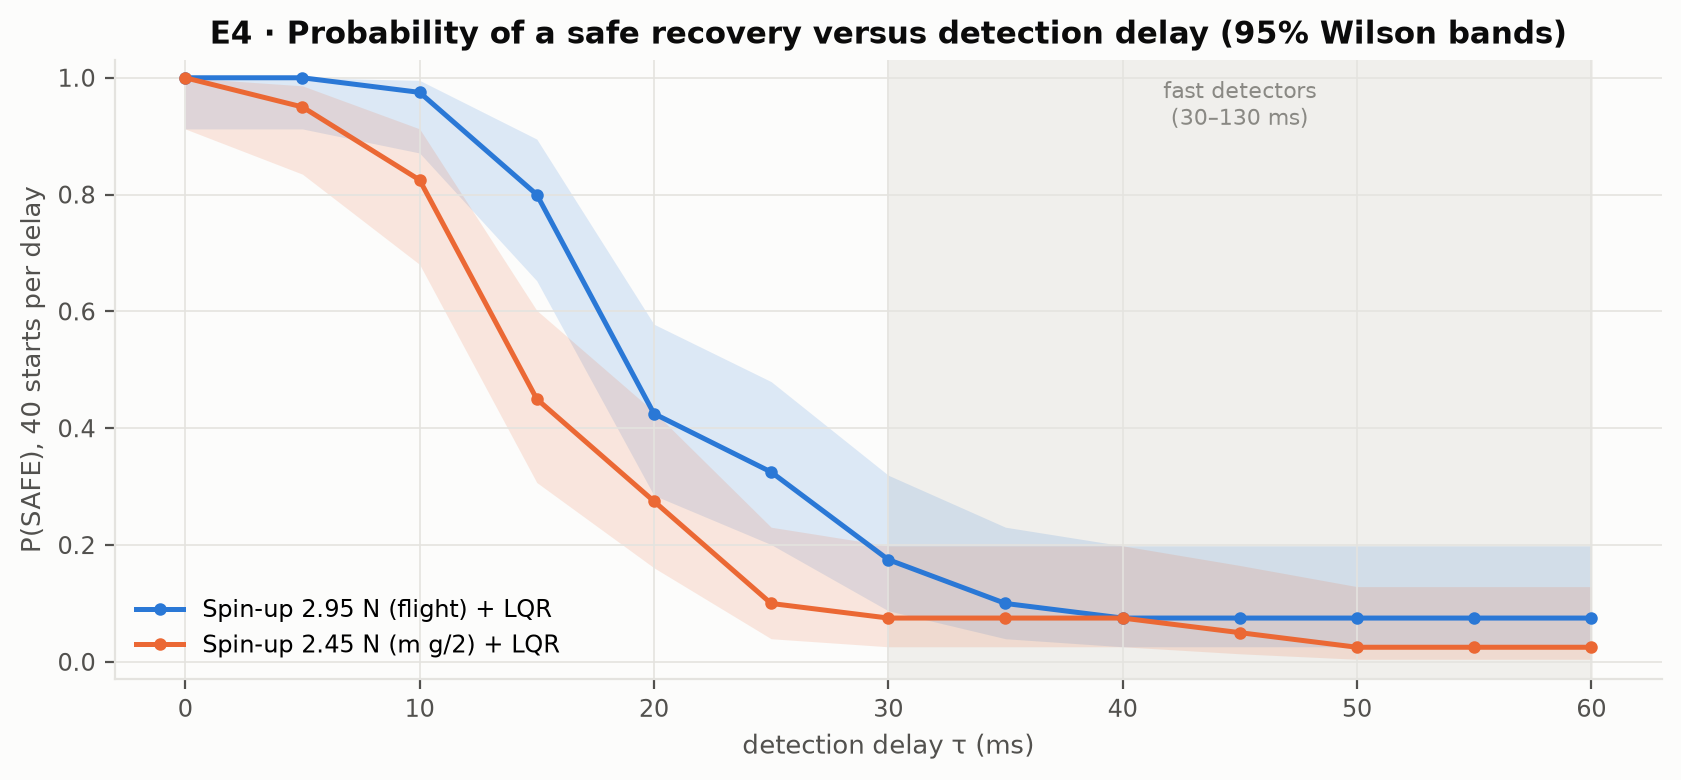
\includegraphics[width=0.85\linewidth]{figures/e4_p_safe.png}
\caption{Probability of a safe recovery against detection delay for the two spin-up thrusts, with 95\% Wilson bands. The shaded region marks the 30 to 130\,ms reported for one fast detector~\cite{strack2021fast}.}\label{fig:psafe}
\end{figure}

\paragraph{Main result.} With the flight spin-up thrust, the probability of a safe recovery falls below 0.9 at about \textbf{12\,ms} of delay and below 0.5 at about \textbf{19\,ms} (Table~\ref{tab:delay}, Figure~\ref{fig:psafe}). With the lower thrust $mg/2$ these are 7 and 14\,ms. If only attitude capture is required (ignoring height loss), the 50\% point moves to 52\,ms (40\,ms with $mg/2$). Published detectors need about 20 to 130\,ms~\cite{strack2021fast,yang2026mml1,zhou2025rotorfailureaware}, so with this strategy a safe recovery is unlikely within the time most current detectors need.

\paragraph{No delay matches the flight.} With the flight thrust and $\tau = 0$, the drone first climbs 0.40\,m and then drops only 0.03\,m below its starting height, qualitatively like the real flight, which climbed about 0.9\,m.

\paragraph{Direct LQR fails.} Switching the failure LQR on directly, without spin-up, captures the attitude in the end but always turns the drone upside down on the way and loses 9 to 16\,m of height, at every delay (Figure~\ref{fig:sweep}). The LQR was designed for a drone that already spins at 19\,rad/s; right after the failure the drone does not spin yet, and the linear model is far from valid there. Section~\ref{sec:certificate} returns to this point.

\begin{figure}[h]
\centering
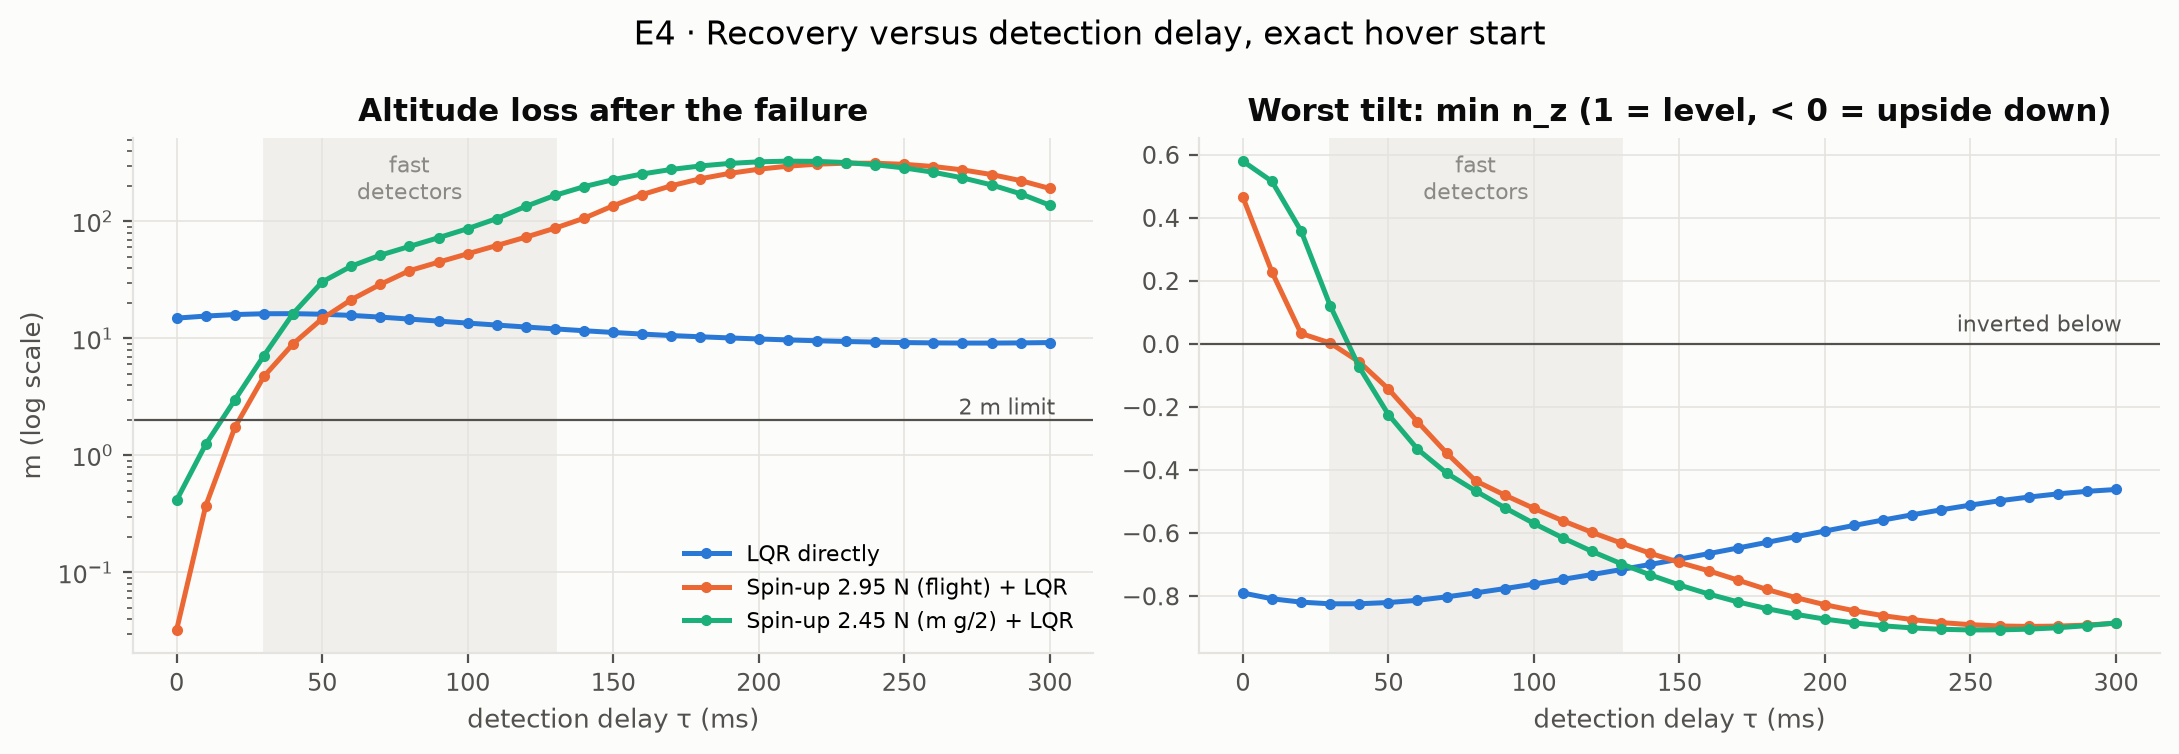
\includegraphics[width=\linewidth]{figures/e4_delay_sweep.png}
\caption{Exact hover start, delays 0 to 300\,ms. Left: height loss (log scale) with the 2\,m limit. Right: the worst tilt, $\min n_z$ (below 0 means upside down).}\label{fig:sweep}
\end{figure}

\begin{figure}[h]
\centering
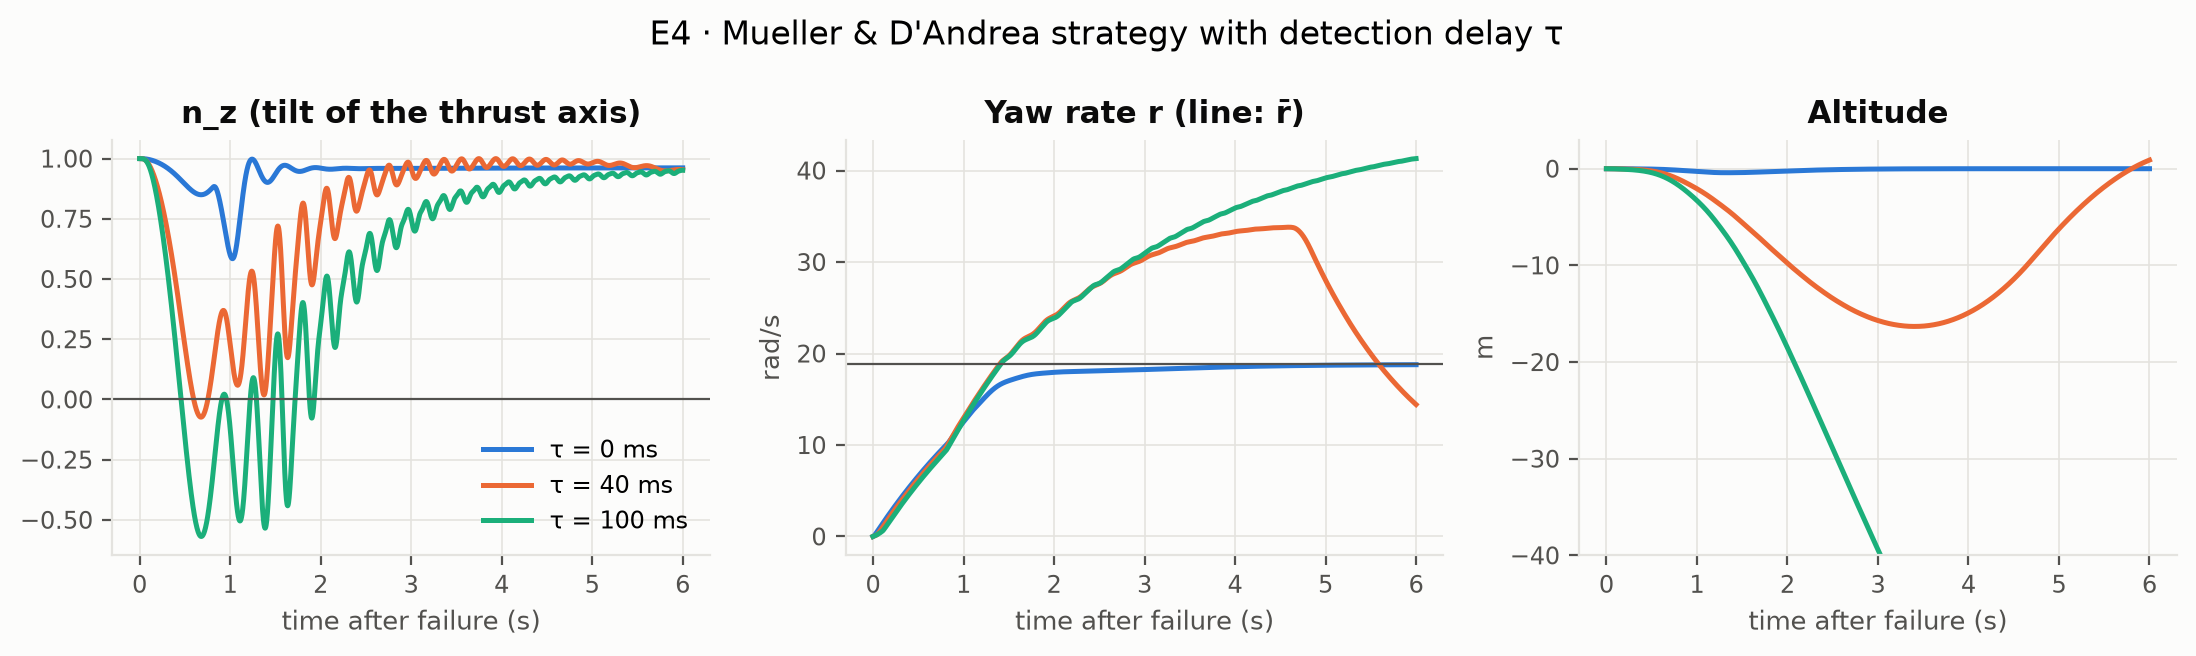
\includegraphics[width=\linewidth]{figures/e4_time_histories.png}
\caption{Spin-up (2.95\,N) then LQR for delays of 0, 20 and 50\,ms: tilt, yaw rate and height.}\label{fig:histories}
\end{figure}

\paragraph{Tuning does not help.} From the exact hover start, every delay up to 20\,ms is safe for all three healthy-controller tunings ($\alpha = 0.3$, 1, 3), and 30\,ms is not. This agrees with the idle-thrust bound: no tuning can stop the roll.

\paragraph{Scope.} These numbers belong to this strategy and this model. In other simulation studies, nonlinear controllers recovered, with some loss of performance, at detection delays of about 0.1 to 0.2\,s~\cite{chen2025learning,zhou2025rotorfailureaware}, so the limit is not a property of rotor loss in general.

\subsection{Do the MPCs tolerate more delay?}
RQ2 asks how the capture controller changes the tolerable delay. As a first look we repeated the scenario on truth plant A with each controller of Section~\ref{sec:mpc} as the capture controller (spin-up at 2.95\,N, then LQR, analytical MPC or residual Koopman MPC). On a mismatched plant a controller designed on the nominal model settles at its own steady state, not at the plant's equilibrium, so capture was judged against each controller's own steady state (found by a 12\,s run from the trim).

\begin{center}\small
\begin{tabular}{lccc}
\toprule
$\tau$ & LQR & MPC, analytical & MPC, residual Koopman \\
\midrule
0\,ms & safe (0.40\,m) & safe (0.53\,m) & safe (0.58\,m) \\
10\,ms & safe (1.69\,m) & inverted (2.52\,m) & inverted (2.80\,m) \\
20\,ms & inverted (6.56\,m) & inverted (8.53\,m) & inverted (7.94\,m) \\
\bottomrule
\end{tabular}
\end{center}
(Height loss in brackets; one run per entry.) LQR is safe up to 10\,ms, both MPCs only without delay. We do not yet understand why. The LQR uses the same linear model and weights, so model validity alone does not explain the difference; candidates are the short 100\,ms horizon and the thrust limits becoming active during capture, where the MPC and the clipped LQR act differently. (All three controllers run at 5\,ms in this comparison.) This needs further study. Note that this table uses plant A and a 5\,ms sample period for every controller (including the healthy one), while Table~\ref{tab:delay} uses the nominal plant and 1\,ms; slower sampling alone adds effective delay, so their absolute numbers are not directly comparable.

%=====================================================================
\section{A first mathematical certificate (RQ2)}\label{sec:certificate}
%=====================================================================
Simulation can only test the starting states we try. A \emph{certificate} is a mathematical proof, checked by a computer, that every state in some set recovers. In this report the certificates are proven for the \emph{linearized} model with thrust limits; how well they carry over to the nonlinear drone is measured by simulation, not proven. RQ2 needs such a set: the \emph{capture set} of the failure controller. If we can show that every state the drone can reach during the undetected phase lies inside the capture set, recovery is guaranteed. This section builds a first capture set (experiment E5) and measures how conservative it is.

\subsection{The idea: an energy-like function that always decreases}
Take the closed loop of the failure LQR on the 10-state linear model, written in deviations from the equilibrium. Without limits it would be $\dot{\vect x} = (A - BK)\vect x$. With the thrust limits it is
\begin{equation}
  \dot{\vect x} = A\vect x + B\operatorname{sat}(F\vect x), \qquad F = -K,
\end{equation}
where $\operatorname{sat}$ clips each input deviation to $[-\bar u_i, \bar u_i]$. Consider the quadratic function $V(\vect x) = \vect x^\top P\vect x$ with $P$ positive definite, and the ellipsoid $\mathcal E = \{\vect x : V(\vect x)\le1\}$. If $V$ decreases along every trajectory that starts in $\mathcal E$, no trajectory can leave $\mathcal E$, and all of them go to the equilibrium. Then $\mathcal E$ is a certified capture set. The question is how to find $P$, and how to handle the clipping, which makes the system nonlinear.

\begin{plain}
Picture a bowl whose bottom is the equilibrium. If we can prove that the drone's state always moves downhill in the bowl, then any state that starts below a certain rim stays below it and slides to the bottom. The certificate is the bowl ($P$) and the rim (the ellipsoid). The thrust limits make the drone weaker when it is far from the bottom, so the rim cannot be arbitrarily high.
\end{plain}

\subsection{Handling the thrust limits (Hu and Lin)}
Hu and Lin~\cite{hu2001saturation} give a sufficient condition based on the following observation. Choose a second, auxiliary gain $H$. If the state is in the region where $|H_i\vect x|\le\bar u_i$ for every input $i$, then the clipped input $\operatorname{sat}(F\vect x)$ is always some mixture (a convex combination) of the vectors
\begin{equation}
  D F\vect x + (I - D)H\vect x, \qquad D \in\mathcal D,
\end{equation}
where $\mathcal D$ is the set of diagonal matrices with 0 or 1 on the diagonal ($2^3 = 8$ of them for three inputs). Each $D$ picks, input by input, either the real gain $F$ or the auxiliary gain $H$. So if $V$ decreases for each of these 8 \emph{linear} systems, it also decreases for the clipped one, inside the region where $|H_i\vect x|\le\bar u_i$.

\subsection{Turning it into LMIs}
For one vertex, ``$V$ decreases at rate at least $2\mu V$'' means
\begin{equation}
  \big(A + B(DF + D^-H)\big)^\top P + P\big(A + B(DF + D^-H)\big) + 2\mu P \preceq 0, \qquad D^- = I - D .
\end{equation}
This contains the product of the unknowns $P$ and $H$, so it is not linear. The standard fix is a change of variables: multiply from both sides by $Q = P^{-1}$ and write $Y = HQ$. The condition becomes
\begin{equation}\label{eq:lmi1}
  AQ + QA^\top + B\big(DFQ + D^-Y\big) + \big(DFQ + D^-Y\big)^\top B^\top + 2\mu Q \preceq -\epsilon I \qquad \forall D\in\mathcal D,
\end{equation}
which is linear in the unknowns $Q$ and $Y$: a linear matrix inequality (we add a small margin $\epsilon$ for numerical safety). The ellipsoid must also lie inside the region where the trick is valid. The largest value of $|H_i\vect x|$ on $\mathcal E$ is $\sqrt{H_iQH_i^\top}$, so we need $H_iQH_i^\top \le \bar u_i^2$, which by a Schur complement is the LMI
\begin{equation}\label{eq:lmi2}
  \begin{pmatrix} \bar u_i^2 & Y_i \\ Y_i^\top & Q \end{pmatrix} \succeq 0, \qquad i = 1, 2, 3 .
\end{equation}
($Y_i$ is row $i$ of $Y$.) Finally, we want the ellipsoid to be large in the direction we care about: from the equilibrium towards $\vect x_{\text{on}}$, the state right after a failure in hover (zero body rates, level attitude, motors at $mg/4$). ``$\beta\vect x_{\text{on}}$ lies in $\mathcal E$'' means $\beta^2\,\vect x_{\text{on}}^\top Q^{-1}\vect x_{\text{on}}\le1$; with $t = 1/\beta^2$ this is again a Schur complement,
\begin{equation}
  \begin{pmatrix} t & \vect x_{\text{on}}^\top \\ \vect x_{\text{on}} & Q\end{pmatrix}\succeq 0,
\end{equation}
and we minimize $t$, which maximizes $\beta$. A value $\beta\ge1$ would mean the failure state itself is certified. (To get a ``general-purpose'' ellipsoid instead, we maximize its volume, $\log\det Q$, under the same constraints.)

Two practical details. The plant's thrust limits are not symmetric around the trim (rotor 2 is at 1.02\,N, between 0.2 and 3.8\,N), but the trick needs symmetric levels, so we take the smaller distance to either limit: $\bar{\vect u} = (1.76, 0.82, 1.76)$\,N; a certificate with these levels also holds for the real limits. And the motor-state deviations must stay within their physical range, so we add $Q_{ii}\le\bar u_i^2$ for the three motor states. Without this bound the problem is badly conditioned: the open-loop model is only marginally stable, and the solver ``certifies'' an almost unbounded, physically meaningless set (tilt deviations above 1, motor deviations above 100\,N).

\begin{codebox}{the certificate in CVXPY}
\begin{lstlisting}
Q = cp.Variable((n, n), symmetric=True);  Y = cp.Variable((m, n))
cons = [Q >> eps * np.eye(n)]
for bits in itertools.product([0, 1], repeat=m):          # the 2^m vertices D
    D = np.diag(bits); Dm = np.eye(m) - D
    M = D @ F @ Q + Dm @ Y
    L = A @ Q + Q @ A.T + B @ M + (B @ M).T + 2 * decay * Q
    cons.append(0.5 * (L + L.T) << -eps * np.eye(n))     # LMI (lmi1)
for i in range(m):
    row = cp.reshape(Y[i, :], (1, n), order="C")
    cons.append(cp.bmat([[np.array([[ubar[i] ** 2]]), row], [row.T, Q]]) >> 0)  # (lmi2)
for i, b in enumerate(box):                               # motor states in range
    if np.isfinite(b): cons.append(Q[i, i] <= b ** 2)
t = cp.Variable()
cons.append(cp.bmat([[cp.reshape(t, (1, 1), order="C"), d.T], [d, Q]]) >> 0)
cp.Problem(cp.Minimize(t), cons).solve(solver="CLARABEL")  # beta = 1/sqrt(t)
\end{lstlisting}
\end{codebox}
The problems are modelled with CVXPY~\cite{diamond2016cvxpy} and solved with the interior-point solver Clarabel~\cite{goulart2024clarabel}, with SCS~\cite{odonoghue2016scs} as a fallback. A test samples 500 points on the boundary of a computed ellipsoid and checks that $V$ really decreases there with the true clipping.

\subsection{Results}
\begin{table}[h]
\centering\small
\caption{Certified ellipsoids for several required decay rates $\mu$. The half-widths are those of the largest-volume ellipsoid (maximizing $\log\det Q$); $\beta$ comes from a second problem that maximizes the extent towards the failure state. $^{*}$Solver status ``optimal\_inaccurate'' (solved to lower accuracy).}\label{tab:cert}
\begin{tabular}{cccccc}
\toprule
$\mu$ (1/s) & $\Delta p, \Delta q, \Delta r$ (rad/s) & $\Delta n_x, \Delta n_y$ & $\Delta z$ (m) & $\beta$ \\
\midrule
0.0$^{*}$ & 2.23, 3.49, 6.20 & 0.42, 0.36 & 3.17 & 0.223 \\
0.1 & 2.17, 3.49, 6.09 & 0.41, 0.35 & 2.99 & 0.221 \\
0.3 & 2.07, 3.50, 5.89 & 0.40, 0.34 & 2.61 & 0.218 \\
0.5 & 1.96, 3.52, 5.76 & 0.38, 0.32 & 2.17 & 0.215 \\
\bottomrule
\end{tabular}
\end{table}

\paragraph{Certified versus simulated.} The certificate covers $\beta\approx0.22$ of the way from the equilibrium to the failure state (Table~\ref{tab:cert}); asking for a faster decay shrinks it only slightly. To see how conservative this is, we started the nonlinear simulation at $\beta\vect x_{\text{on}}$ for $\beta = 0.1, 0.2, \dots, 1.0$ with the failure LQR and no delay. Every start up to $\beta = 0.7$ recovered without turning over (height loss 0.42\,m at 0.7); at 0.8 and 0.9 the attitude was captured but the drone turned over, and at 1.0 it was not captured. So the certificate is about three times conservative in this direction, and this LQR on its own cannot recover safely from the failure state itself, which is why the spin-up phase is needed.

\paragraph{Where the controller fails.} We also simulated a $21\times21$ grid of starting points in the plane of yaw-rate deviation $\Delta r$ and tilt deviation $\Delta n_y$, all other states at equilibrium (Figure~\ref{fig:cert}). 376 of 441 points recovered without turning over; 7\% of these lie inside the certified slice, the rest is the conservatism gap. All failures occur at spin rates of 4.8\,rad/s or less, and none at 6.8\,rad/s or more. In other words, the LQR works well as long as the drone already spins reasonably fast, and fails when it starts from a slow spin, which is exactly the situation right after a failure. A certificate built from one linearization at the full spin (19\,rad/s) cannot reach that region.

\begin{figure}[h]
\centering
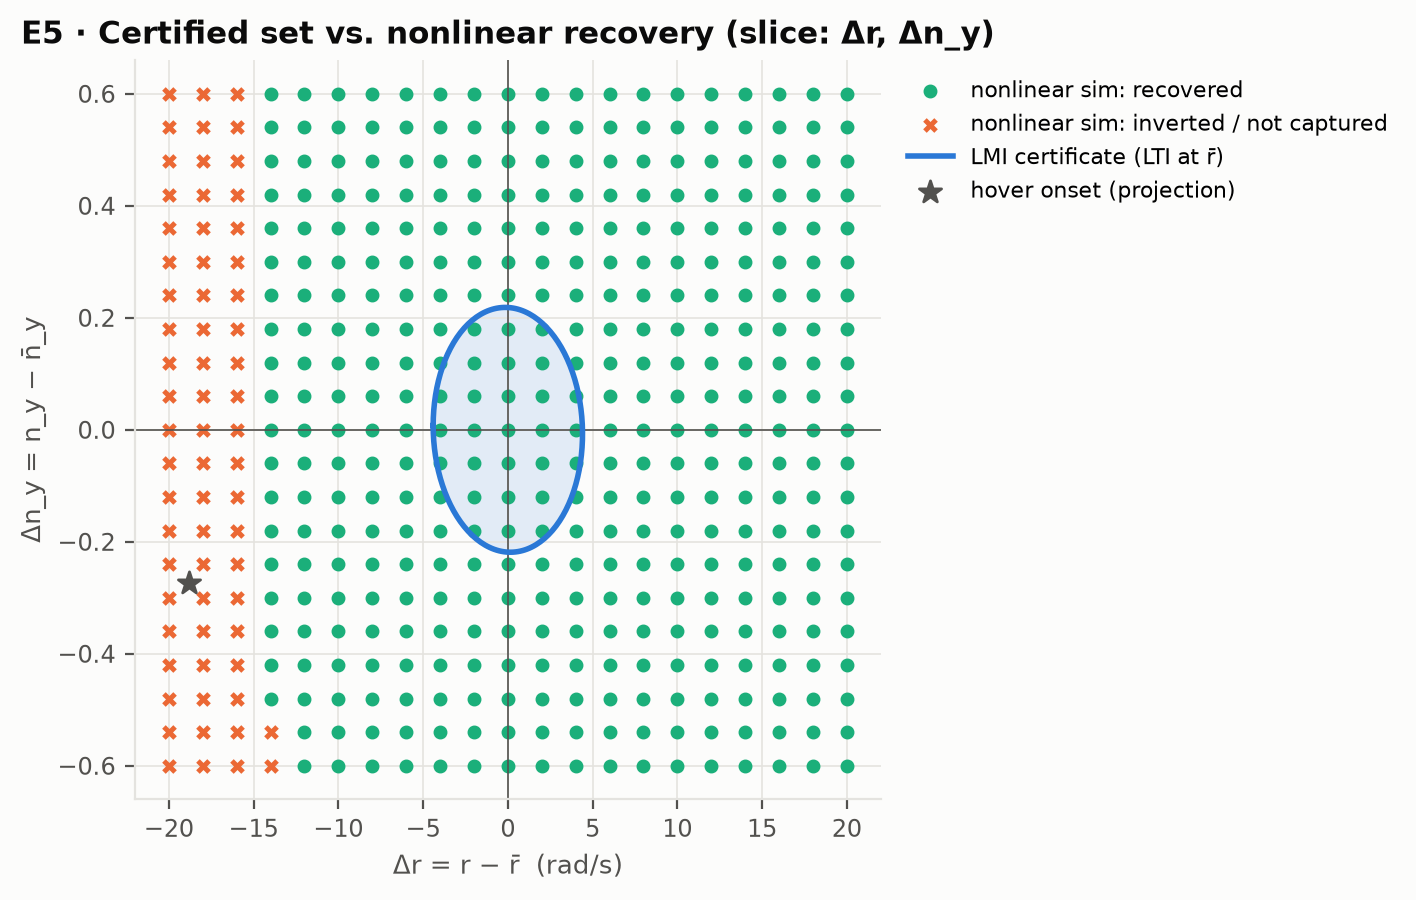
\includegraphics[width=0.75\linewidth]{figures/e5_certificate_slice.png}
\caption{Slice $(\Delta r, \Delta n_y)$ of the certified ellipsoid ($\mu = 0.1$\,s$^{-1}$) against a grid of nonlinear simulations. Dots: recovered; crosses: turned over or not captured; star: projection of the failure state (labelled ``hover onset'' in the plot). ``LTI at $\bar r$'' means the certificate uses the linear model at the equilibrium yaw rate.}\label{fig:cert}
\end{figure}

\subsection{From here to a certified delay budget (planned)}
The results point to the next steps, which are not implemented yet:
\begin{enumerate}
  \item \textbf{A certificate over the whole spin-up.} If the other operating-point values are held fixed, the linearized matrix depends affinely on the yaw rate $r$ (otherwise they become additional scheduling parameters, and linearizing away from an equilibrium adds a drift term). Treating $r$ as a parameter in an interval $[r_{\text{onset}}, \bar r + \delta]$ and requiring the LMIs~\eqref{eq:lmi1} at the two ends with a common $Q$ (a linear parameter-varying, LPV, certificate) would certify the whole interval. LPV synthesis on the yaw rate~\cite{stephan2018lpv} and recoverable sets at the relaxed hover~\cite{qi2016recoverable} exist; our aim is to use such a set as the capture target of a delay budget.
  \item \textbf{The reachable set of the undetected phase.} During the delay the drone obeys an \emph{affine} linear model (linear plus a constant term) $\dot{\vect x} = A_f\vect x + \vect d$ (healthy controller, rotor 4 missing; $\vect d$ is the constant push from the missing thrust). Starting from an ellipsoid $\mathcal X_0$ of pre-failure states, the states reachable at time $\tau$ form the shifted ellipsoid $\mathcal R(\tau) = e^{A_f\tau}\mathcal X_0 \oplus \{\int_0^\tau e^{A_f s}\vect d\,ds\}$, where $\oplus$ (the Minkowski sum) adds the fixed shift to every point of the set.
  \item \textbf{The certified delay.} $\tau^\star = \sup\{\tau : M\mathcal R(\tau)\subseteq\mathcal C\}$, where $M$ maps healthy-flight states to failure-controller coordinates and $\mathcal C$ is the capture set. Containment of one ellipsoid in another can be written as an LMI by the S-procedure (a standard way to turn ``one quadratic inequality implies another'' into a matrix inequality), and $\tau^\star$ is found by bisection.
\end{enumerate}
The main risk is that a single quadratic function over the whole spin-up is infeasible or too conservative; the fallbacks are a parameter-dependent Lyapunov function, or a chain of nested ellipsoids along the spin-up.

%=====================================================================
\section{Discussion, limitations and next steps}\label{sec:discussion}
%=====================================================================
\subsection{Status of the hypotheses}
\begin{table}[H]
\centering\small
\caption{Status of the hypotheses of Section~\ref{sec:intro}.}\label{tab:hyp}
\begin{tabularx}{\linewidth}{l L p{5.6cm}}
\toprule
& Hypothesis & Status \\
\midrule
H1 & Full-state EDMDc on the failed drone is unstable and loses to ``no change'' at long horizons & Supported (4 of 55 eigenvalues slightly outside the unit circle) \\
H2 & The residual model predicts best & Supported from 100\,ms to 1\,s, on the training plant only (beyond about 2\,s ``no change'' is better) \\
H3 & Residual Koopman MPC removes the steady bias under mismatch & Partly: reduced by 32\% on the training plant; worse on one held-out variant \\
H4 & The residual model needs less data & Supported (10 episodes beat 40) \\
H5 & The linear certificate does not contain the failure state; one over the spin-up does & First half supported ($\beta = 0.22$); second half not yet tested \\
H6 & The certified $\tau^\star$ is finite and of the order of real detector delays & Not yet tested; the empirical limit (12 to 19\,ms) is shorter than detectors need \\
H7 & The certified $\tau^\star$ is within 2 to 3 times the empirical value & Not yet tested \\
\bottomrule
\end{tabularx}
\end{table}

\subsection{What the results mean}
\paragraph{Physics first, learning second.} The physics model of Mueller and D'Andrea, which we reproduced to every printed digit except in one internally inconsistent published case, already describes the spinning drone well: it gives the right equilibrium, the right flight spin-up time and a controller that works. Learning helps only in the second order, and only when the learned part is restricted to the error. Learning everything from data produced an unstable model, as our proposal predicted.

\paragraph{A calibration, not yet a general model.} The learned residual is accurate on the plant it saw and harmful on a different plant. As it stands it behaves like an offline calibration of one vehicle. Online adaptation, or a residual that also uses a short history of states, is needed before it can be called a general correction for rotor failure.

\paragraph{Detection time is the bottleneck.} The most striking result is how little detection delay the published strategy tolerates in our simulation: around 10 to 20\,ms, while published detectors need about 20 to 130\,ms. The cause is simple and robust: the healthy controller cannot stop the roll because the opposite rotor cannot go below idle thrust. This makes a certified delay budget, and controllers that tolerate longer delays, practically important.

\subsection{Limitations}
\begin{enumerate}
  \item \textbf{Spin-up thrust.} The delay tolerance depends on the spin-up thrust (12 against 7\,ms for the 90\% level). The flight value is read from a plot and carries some uncertainty.
  \item \textbf{Nominal plant for the delay study.} The delay study uses the nominal plant; the published models over-predict the steady spin rate in flight by about 20 to 27\%.
  \item \textbf{Generalization.} The residual model helps reliably only on the plant family it was trained on.
  \item \textbf{Linear certificates.} The certificate holds for the linearized loop with saturation. The gap to the nonlinear system is measured by simulation, not proven.
  \item \textbf{Truth-plant realism.} The truth plants add thrust loss, inertia error and motor lag, but not yet air-relative thrust or quadratic drag, both of which we validated in our implementation of the IJRR model. There is no sensor noise and no translational drag yet.
  \item \textbf{Certificate for the learned controller.} The clipping level $\vect d_{\max}$ is a percentile of the training residuals, not a bound on the true mismatch, and a constrained MPC needs more than the saturation conditions of Section~\ref{sec:certificate}. Both must be addressed before the residual Koopman loop can be certified.
  \item \textbf{Simulation only.} No result has been tested on hardware.
  \item \textbf{Full-state measurement.} All controllers are given the exact state. A real spinning drone needs an estimator for the tilt, height and vertical speed, and sensor noise will affect both the learned residual and the MPC.
  \item \textbf{Closed-loop data.} The learning data are recorded under LQR feedback with added excitation, which correlates states and inputs; possible bias from this is not analysed.
  \item \textbf{Missing baselines.} An offset-free (integral-action) MPC is the obvious classical alternative for removing a steady error, and grey-box estimation of the few uncertain physical parameters (thrust loss, inertias, motor time constant) is the obvious model-based alternative to a black-box residual. Neither has been compared yet.
  \item \textbf{Literature access.} Several closely related papers~\cite{stephan2018lpv,lanzon2014flight,qi2016recoverable,basak2015switching} have not yet been read in full; our statements about them rely on abstracts, a thesis and citing papers.
\end{enumerate}

\subsection{Plan for the remaining weeks}
The course has a final progress presentation on 31 October 2026, and the journal-style final report is due on 13 November 2026.
\begin{table}[h]
\centering\small
\begin{tabularx}{\linewidth}{l L}
\toprule
Dates & Work \\
\midrule
Until 18 Oct & LPV model in the yaw rate and a saturation-aware certificate over the spin-up. MPC on the full-state Koopman model (the second controller of our proposal) and an integral-action MPC baseline. Read the remaining key papers in full. \\
19 to 25 Oct & Reachable set of the undetected phase and the containment test, giving a first certified $\tau^\star$; comparison with the empirical curve. Online adaptation of the residual by recursive least squares. \\
26 to 31 Oct & Sensitivity of $\tau^\star$ to the spin-up thrust, idle thrust and motor lag; air-relative thrust in the truth plant. Final progress presentation on 31 Oct. \\
1 to 13 Nov & Bound on the true model mismatch and a certificate for the residual Koopman loop if time allows; final simulations and the journal-style report, due 13 Nov. \\
\bottomrule
\end{tabularx}
\end{table}

\subsection{Conclusion}
We built a simulator of a quadrotor with complete rotor loss and showed that it reproduces three published papers and the spin-up time of a real flight. On the plant it was trained on, a Koopman model that learns only the error of the physics model is the most accurate predictor from 100\,ms to 1\,s, needs less data than a Koopman model of the full dynamics, and reduces a steady altitude error by one third inside a convex MPC; it does not yet carry over to a plant with different parameters. In our simulation, the published recovery strategy recovers safely with high probability only for detection delays of about 10 to 20\,ms, shorter than most published detectors need (about 20 to 130\,ms), because nothing can stop the roll while the failure is undetected. A first LMI certificate covers 22\% of the way to the failure state, and the controller fails only at low spin rates, which points to a certificate over the spin-up as the next step. The remaining weeks build that certificate and the certified delay budget, and evaluate each capture controller, including the residual Koopman MPC, by the delay it tolerates.


\appendix
%=====================================================================
\section{Glossary}\label{app:glossary}
%=====================================================================
Terms in alphabetical order. The section where each is first used in detail is given in brackets.

\small
\begin{longtable}{p{0.24\linewidth}p{0.70\linewidth}}
\toprule
Term & Meaning \\
\midrule
\endhead
Actuator & A device that acts on the system; here the four motor--propeller units. \\
Affine & Linear plus a constant term, $A\vect x + \vect d$. \\
Air-relative thrust & Propeller thrust computed from the propeller's speed relative to the air ($\Omega_i + r$) rather than relative to the body; matters when the body spins fast (\ref{sec:val-ijrr}). \\
Algebraic Riccati equation & The matrix equation whose solution $P$ gives the optimal LQR gain; ``discrete'' version (DARE) for sampled systems (\ref{sec:background}, \ref{sec:mpc}). \\
Attainable moment set & The set of torques the remaining rotors can produce within their thrust limits. \\
Body frame & Coordinate frame fixed to the drone (\ref{sec:model}). \\
Body rates $(p,q,r)$ & Rotation rates about the body $x$, $y$, $z$ axes: roll rate, pitch rate, yaw rate. \\
Brent's method & A reliable one-dimensional root finder that needs a bracket where the function changes sign (\ref{sec:model}). \\
Bryson's rule & Choosing LQR weights as $1/(\text{largest acceptable value})^2$ (\ref{sec:linear}). \\
Capture & Bringing the drone into the relaxed hover after a failure; a ``capture controller'' does this (\ref{sec:delay}). \\
Capture set & A set of states from which the capture controller is proven to recover (\ref{sec:certificate}). \\
Central differences & Numerical derivative $(f(x+\epsilon) - f(x-\epsilon))/2\epsilon$ (\ref{sec:background}). \\
Certificate & A computer-checked mathematical proof that a property (here, recovery) holds for a whole set of states (\ref{sec:certificate}). \\
Closed loop & The system together with its feedback controller. \\
Controllability & Whether the inputs can steer the state anywhere; tested by the rank of $[B, AB, \dots]$ or the PBH test (\ref{sec:linear}). \\
Convex problem & An optimization problem in which every local minimum is a global one, so solvers find the best solution reliably; QPs with positive semidefinite cost and LMI problems are convex. With a strictly convex cost the solution is unique. \\
CVXPY & A Python library for writing convex optimization problems; it passes them to solvers such as OSQP or Clarabel. \\
Damping ratio $\zeta$ & How quickly an oscillation dies out; 0 means never, 1 means no overshoot. \\
Delay margin & The largest pure input delay a feedback loop tolerates before becoming unstable (\ref{sec:linear}). \\
Detection delay $\tau$ & Time between the rotor failure and the moment the flight computer knows about it (\ref{sec:delay}). \\
Dictionary & The list of functions (observables) used to lift the state in EDMD (\ref{sec:koopman}). \\
EDMD / EDMDc & Extended dynamic mode decomposition (with control): fitting a linear model on a dictionary of functions of the state by least squares (\ref{sec:background}). \\
Eigenvalue & A number $\lambda$ with $A\vect v = \lambda\vect v$; describes one mode of a linear system (\ref{sec:background}). \\
Equilibrium (trim) & A state and input at which nothing changes (\ref{sec:background}). \\
Euler angles & Roll $\phi$, pitch $\theta$, yaw $\psi$: three angles that describe orientation; break down at some orientations (gimbal lock). \\
Excitation & Random changes added to the inputs during data collection so that the data show how the system responds (\ref{sec:koopman}). \\
FDI / FDD & Fault detection and isolation / diagnosis: algorithms that notice and locate a failure. \\
Feedback linearization & A nonlinear control method that cancels the nonlinear terms by the control input so the remaining loop is linear. \\
Floquet theory & Stability theory for linear systems whose coefficients repeat periodically in time (\ref{sec:model}). \\
FTC & Fault-tolerant control: control that keeps working after a failure. Active FTC switches controller after detection; passive FTC does not need detection. \\
Gramian & A matrix measuring how strongly each direction of the state can be reached (controllability) or seen (observability) in a given time (\ref{sec:linear}). \\
Gyroscopic effect & The torque needed to change the direction of an angular momentum; makes spinning bodies precess (\ref{sec:model}). \\
$H_\infty$ loop shaping & A robust linear control design that shapes the loop's frequency response and maximizes a robustness margin. \\
Healthy controller & The normal controller used with four working rotors. \\
Horizon & How far ahead MPC predicts (here 20 steps, 100\,ms). \\
INDI & Incremental nonlinear dynamic inversion: a nonlinear control method that uses measured accelerations. \\
Inertia matrix & How hard it is to change the rotation of a body about each axis. \\
Interior-point method & A family of algorithms for convex optimization that moves through the inside of the feasible set; Clarabel is one. \\
Invariant set & A set that no trajectory starting inside it can leave (\ref{sec:certificate}). \\
Jacobian & Matrix of partial derivatives; the linearization of a nonlinear function (\ref{sec:background}). \\
Koopman operator & A linear operator that advances functions of the state in time; lets nonlinear systems be described linearly in a lifted space (\ref{sec:background}). \\
Lifted state & The vector of dictionary functions $\vect z = \psi(\vect x)$. \\
LMI & Linear matrix inequality: a convex constraint saying a matrix, linear in the unknowns, is positive or negative semidefinite (\ref{sec:certificate}). \\
LPV & Linear parameter-varying: a linear model whose matrices depend on a measured, changing parameter (here the yaw rate). \\
LQR & Linear-quadratic regulator: the state-feedback gain minimizing a quadratic cost (\ref{sec:background}). \\
LTI & Linear time-invariant: a model $\dot{\vect x} = A\vect x + B\vect u$ with constant matrices. \\
Lyapunov function & An energy-like function that decreases along the motion; its existence proves stability (\ref{sec:certificate}). \\
Measured disturbance & A known, additive term in an MPC prediction model; used here for the learned residual (\ref{sec:mpc}). \\
Minkowski sum $\oplus$ & The set of all sums $a + b$ with $a$ from one set and $b$ from another (\ref{sec:certificate}). \\
Monte Carlo & Repeating a simulation from many random starts to estimate probabilities (\ref{sec:delay}). \\
Motor lag & Delay of the motor thrust behind its command, modelled as a first-order lag with time constant $\sigma$ (\ref{sec:model}). \\
MPC & Model predictive control: repeatedly optimize the inputs over a short future horizon and apply the first one (\ref{sec:background}, \ref{sec:mpc}). \\
NMPC & Nonlinear MPC: MPC with a nonlinear prediction model (no longer a QP). \\
Normalized RMSE & Root mean square error after dividing each state by its typical size (\ref{sec:koopman}). \\
Observability & Whether the state can be worked out from the sensor outputs (\ref{sec:linear}). \\
Offset-free MPC & MPC that estimates a constant disturbance and compensates it, removing steady errors like integral action. \\
Open loop & Without feedback; an open-loop prediction uses no later measurements. \\
Operator splitting & A way of solving an optimization problem by alternating between simpler subproblems; used by OSQP. \\
OSQP & A fast solver for quadratic programs. \\
Overfitting & Fitting the noise or quirks of the training data instead of the true pattern. \\
PBH test & Popov--Belevitch--Hautus test: checks controllability (or observability) mode by mode (\ref{sec:linear}). \\
Plant & The system being controlled (here the drone, or a truth plant in simulation). \\
Positive definite & A symmetric matrix $P$ with $\vect x^\top P\vect x>0$ for all $\vect x\ne0$, written $P\succ0$; $\succeq$ allows equality (\ref{sec:background}). \\
QP & Quadratic program: minimize a quadratic cost subject to linear constraints; convex. \\
Quaternion & Four numbers that describe an orientation without gimbal lock (\ref{sec:model}). \\
Randomized plants & Training on many plants with randomly drawn parameters, also called domain randomization (\ref{sec:koopman}). \\
Reaction torque & Twisting torque on the body from a spinning propeller (\ref{sec:intro}). \\
Reduced attitude $\vect n$ & The inertial ``up'' direction seen in body axes, $R^\top\vect e_3$; all that is controlled after the failure (\ref{sec:model}). \\
Relaxed hover & The spinning equilibrium of a multicopter that has lost rotors (\ref{sec:model}). \\
Residual & The difference between the truth and the physics model's prediction (\ref{sec:koopman}). \\
Ridge regression & Least squares with a penalty on the size of the coefficients (\ref{sec:background}). \\
RK4 & The classical fourth-order Runge--Kutta integration method (\ref{sec:background}). \\
Rotation matrix $R$ & Matrix turning body-frame vectors into inertial-frame vectors. \\
Saturation & Clipping of an input at its physical limits (\ref{sec:background}). \\
Schur complement & A rule that turns certain nonlinear matrix inequalities into LMIs (\ref{sec:certificate}). \\
SE(3) & The set of all positions and orientations of a rigid body. \\
Singular values & Numbers that measure how much a matrix stretches vectors in each direction; a value near zero means a direction the matrix almost loses. \\
Sliding-mode control & A robust nonlinear control method that forces the state onto a chosen surface by switching control. \\
Spectral radius & The largest eigenvalue magnitude of a discrete-time matrix; above 1 means growth. \\
Spin-up & Flying on two opposing rotors with no attitude feedback until the drone spins fast enough for the failure LQR (\ref{sec:delay}). \\
S-procedure & A standard technique that turns ``one quadratic inequality implies another'' into an LMI (\ref{sec:certificate}). \\
Standardize & Subtract the mean and divide by the standard deviation. \\
State & The smallest set of numbers that determines the future of a system given its inputs (\ref{sec:background}). \\
Sum-of-squares (SOS) programming & An extension of LMI methods that certifies polynomial inequalities, used for nonlinear stability regions. \\
Supervisor & The logic that switches from the healthy to the failure controller after detection (\ref{sec:delay}). \\
Switched system & A system that jumps between several models, for example healthy and faulty; ``dwell time'' is the minimum average time between switches for which stability is guaranteed. \\
Thrust & The upward force of a propeller, $f = \kappa_f\Omega^2$. \\
Truth plant & A simulated plant with effects the nominal model lacks, used to generate data and to test controllers (\ref{sec:truth}). \\
Wilson interval & A confidence interval for a probability estimated from a count (\ref{sec:delay}). \\
Zero-order hold (ZOH) & Holding a digital command constant until the next sample (\ref{sec:background}). \\
\bottomrule
\end{longtable}
\normalsize

%=====================================================================
\section{Symbols}\label{app:symbols}
%=====================================================================
\small
\begin{longtable}{p{0.18\linewidth}p{0.55\linewidth}p{0.18\linewidth}}
\toprule
Symbol & Meaning & Value / unit \\
\midrule
\endhead
$m$ & mass & 0.50\,kg \\
$g$ & gravity & 9.81\,m/s$^2$ \\
$l$ & arm length & 0.17\,m \\
$I^B$, $I^T$, $I^P$ & inertia of body, body with propellers, one propeller & kg\,m$^2$ \\
$\kappa_f$ & thrust coefficient, $f = \kappa_f\Omega^2$ & $6.41\times10^{-6}$\,N\,s$^2$/rad$^2$ \\
$\kappa_\tau$ & reaction torque per unit thrust & 0.0169\,m \\
$\gamma$ & linear yaw-drag coefficient & $2.75\times10^{-3}$\,N\,m\,s/rad \\
$f_i$, $f_\Sigma$ & thrust of rotor $i$, total thrust & N \\
$f_{\min}$, $f_{\max}$ & running-motor thrust limits & 0.2, 3.8\,N \\
$\sigma$ & motor time constant & 15\,ms \\
$u_i$ & thrust command of rotor $i$ & N \\
$\Omega_i$, $\Omega_\Sigma$ & signed speed of propeller $i$, and their sum & rad/s \\
$\vect d$, $\vect v$ & position and velocity (inertial frame) & m, m/s \\
$R$, $\vect q$ & rotation matrix and quaternion (body to inertial) & \\
$\vect\omega = (p,q,r)$ & body rates & rad/s \\
$\vect n = R^\top\vect e_3$ & reduced attitude & \\
$\vect e_3$ & $(0,0,1)$ & \\
$\eta$, $k$ & thrust efficiency $1 - k\|\vect\omega\|^2$ and its coefficient & s$^2$/rad$^2$ \\
$\rho$ & thrust ratio $f_2/f_1$ at the relaxed hover & 0.5 \\
$\bar{(\cdot)}$ & value at the equilibrium & \\
$\bar a$ & gyroscopic coupling constant & $-10.10$\,rad/s \\
$A, B$ & continuous-time linear model & \\
$A_d, B_d$ & discrete-time (ZOH) model & \\
$\Ts$ & sample period of learning and MPC & 5\,ms \\
$K$, $F=-K$ & feedback gain & \\
$Q, R$ & LQR / MPC weights (Section~\ref{sec:certificate}: $Q = P^{-1}$) & \\
$P$, $P_N$ & Riccati solution / Lyapunov matrix; MPC terminal cost & \\
$N$ & MPC horizon & 20 steps \\
$\hat{\vect f}$ & filtered-command estimate of the motor thrusts & N \\
$\vect\xi$, $\psi$, $\vect\zeta$ & learning features, dictionary, lifted state & \\
$W$, $\vect d_{\max}$ & residual regression matrix, clipping level & \\
$\tau$, $\tau^\star$ & detection delay, certified maximum delay & ms \\
$\bar{\vect u}$ & symmetric saturation levels & (1.76, 0.82, 1.76)\,N \\
$\mu$ & required decay rate in the certificate & 1/s \\
$\beta$ & certified fraction of the way to the failure state & \\
$\alpha$ & aggressiveness factor of the healthy LQR & \\
\bottomrule
\end{longtable}
\normalsize

%=====================================================================
\section{Software and reproducibility}\label{app:repro}
%=====================================================================
The simulator, analysis and experiments are written in Python with NumPy~\cite{harris2020numpy}, SciPy~\cite{virtanen2020scipy} and Matplotlib~\cite{hunter2007matplotlib}. Convex problems are modelled with CVXPY~\cite{diamond2016cvxpy} and solved with Clarabel~\cite{goulart2024clarabel}, SCS~\cite{odonoghue2016scs} and OSQP~\cite{stellato2020osqp}; tests use pytest~\cite{pytest}. Package versions are pinned in \texttt{requirements.txt}. The code is available at \url{https://github.com/pranshuk22/quadrotor-rotor-loss-recovery}.

\begin{verbatim}
python3 -m venv .venv && .venv/bin/pip install -r requirements.txt
.venv/bin/python -m pytest -q        # 46 pass + 1 expected failure
.venv/bin/python experiments/v0_validation_report.py
.venv/bin/python experiments/e1_equilibrium.py   # and e2 ... e7
\end{verbatim}

\begin{table}[h]
\centering\small
\begin{tabularx}{\linewidth}{l l L l}
\toprule
ID & Script & Question & Runtime \\
\midrule
V0 & \texttt{v0\_validation\_report.py} & Does the model match published numbers and flight data? & seconds \\
E1 & \texttt{e1\_equilibrium.py} & Relaxed hover against the paper; $\rho$ sweep & seconds \\
E2 & \texttt{e2\_structure.py} & Eigenvalues, controllability, observability by sensor set & seconds \\
E3 & \texttt{e3\_lqr.py} & LQR designs, delay margins, nonlinear checks & about 15\,s \\
E4 & \texttt{e4\_delay\_sweep.py} & Effect of detection delay (Monte Carlo) & several minutes \\
E5 & \texttt{e5\_first\_certificate.py} & LMI certificate and its conservatism & about 8\,min \\
E6 & \texttt{e6\_koopman\_prediction.py} & Physics vs full-state vs residual EDMDc & about 2.5\,min \\
E7 & \texttt{e7\_mpc\_closed\_loop.py} & LQR vs analytical MPC vs residual Koopman MPC & about 3\,min \\
\bottomrule
\end{tabularx}
\end{table}
Each script writes a table to \texttt{results/tables/} and figures to \texttt{results/figures/}; all random seeds are fixed in the scripts (for example seeds 11, 12, 13 and 21 for the training, test and randomized data of E6). Runtimes are for an 8-core laptop.


\bibliographystyle{unsrtnat}
\bibliography{references}

\end{document}
